% $Header: /cvsroot/latex-beamer/latex-beamer/doc/beamercolorthemeexample.tex,v 1.11 2004/10/07 20:53:04 tantau Exp $
\documentclass{beamer}\usepackage[]{graphicx}\usepackage[]{color}
%% maxwidth is the original width if it is less than linewidth
%% otherwise use linewidth (to make sure the graphics do not exceed the margin)
\makeatletter
\def\maxwidth{ %
  \ifdim\Gin@nat@width>\linewidth
    \linewidth
  \else
    \Gin@nat@width
  \fi
}
\makeatother

\definecolor{fgcolor}{rgb}{0.345, 0.345, 0.345}
\newcommand{\hlnum}[1]{\textcolor[rgb]{0.686,0.059,0.569}{#1}}%
\newcommand{\hlstr}[1]{\textcolor[rgb]{0.192,0.494,0.8}{#1}}%
\newcommand{\hlcom}[1]{\textcolor[rgb]{0.678,0.584,0.686}{\textit{#1}}}%
\newcommand{\hlopt}[1]{\textcolor[rgb]{0,0,0}{#1}}%
\newcommand{\hlstd}[1]{\textcolor[rgb]{0.345,0.345,0.345}{#1}}%
\newcommand{\hlkwa}[1]{\textcolor[rgb]{0.161,0.373,0.58}{\textbf{#1}}}%
\newcommand{\hlkwb}[1]{\textcolor[rgb]{0.69,0.353,0.396}{#1}}%
\newcommand{\hlkwc}[1]{\textcolor[rgb]{0.333,0.667,0.333}{#1}}%
\newcommand{\hlkwd}[1]{\textcolor[rgb]{0.737,0.353,0.396}{\textbf{#1}}}%
\let\hlipl\hlkwb

\usepackage{framed}
\makeatletter
\newenvironment{kframe}{%
 \def\at@end@of@kframe{}%
 \ifinner\ifhmode%
  \def\at@end@of@kframe{\end{minipage}}%
  \begin{minipage}{\columnwidth}%
 \fi\fi%
 \def\FrameCommand##1{\hskip\@totalleftmargin \hskip-\fboxsep
 \colorbox{shadecolor}{##1}\hskip-\fboxsep
     % There is no \\@totalrightmargin, so:
     \hskip-\linewidth \hskip-\@totalleftmargin \hskip\columnwidth}%
 \MakeFramed {\advance\hsize-\width
   \@totalleftmargin\z@ \linewidth\hsize
   \@setminipage}}%
 {\par\unskip\endMakeFramed%
 \at@end@of@kframe}
\makeatother

\definecolor{shadecolor}{rgb}{.97, .97, .97}
\definecolor{messagecolor}{rgb}{0, 0, 0}
\definecolor{warningcolor}{rgb}{1, 0, 1}
\definecolor{errorcolor}{rgb}{1, 0, 0}
\newenvironment{knitrout}{}{} % an empty environment to be redefined in TeX

\usepackage{alltt}

\usepackage{beamerthemesplit}
\usepackage{graphicx,amsmath,natbib} %,apalike,cite
\usepackage{color}
\usepackage{subfigure}
%\usepackage{graphicx,times,amsmath}

\usetheme{Frankfurt}
\usecolortheme{seahorse}
\usecolortheme{rose}

\newcommand{\bfalpha} {\boldsymbol{\alpha}}
\newcommand{\bfbeta} {\boldsymbol{\beta}}
\newcommand{\bfgamma} {\boldsymbol{\gamma}}
\newcommand{\bfdelta} {\boldsymbol{\delta}}
\newcommand{\bfepsilon} {\boldsymbol{\epsilon}}
\newcommand{\bfxi} {\boldsymbol{\xi}}
\newcommand{\bfpi} {\boldsymbol{\pi}}
\newcommand{\bfmu} {\boldsymbol{\mu}}
\newcommand{\bfsigma} {\boldsymbol{\sigma}}
\newcommand{\bfeta} {\boldsymbol{\eta}}
\newcommand{\bfzeta} {\boldsymbol{\zeta}}
\newcommand{\bfvarphi} {\boldsymbol{\varphi}}
\newcommand{\bflambda} {\boldsymbol{\lambda}}
\newcommand{\bfpsi} {\boldsymbol{\psi}}
\newcommand{\bfphi} {\boldsymbol{\phi}}
\newcommand{\bfvarpsi} {\boldsymbol{\varpsi}}
\newcommand{\bfnu} {\boldsymbol{\nu}}
\newcommand{\bftheta} {\boldsymbol{\theta}}
\newcommand{\bfTheta} {\boldsymbol{\Theta}}
\newcommand{\bfOmega} {\boldsymbol{\Omega}}
\newcommand{\bfSigma} {\boldsymbol{\Sigma}}
\newcommand{\bfLambda} {\boldsymbol{\Lambda}}
\newcommand{\bfchi} {\boldsymbol{\chi}}
\newcommand{\bfvartheta} {\boldsymbol{\vartheta}}

\newcommand{\bfs} {\mathbf{s}}
\newcommand{\bfu} {\mathbf{u}}
\newcommand{\bfv} {\mathbf{v}}
\newcommand{\bfx} {\mathbf{x}}
\newcommand{\bfy} {\mathbf{y}}
\newcommand{\bfD} {\mathbf{D}}
\newcommand{\bfP} {\mathbf{P}}
\newcommand{\bfX} {\mathbf{X}}
\newcommand{\bfM} {\mathbf{M}}
\newcommand{\bfY} {\mathbf{Y}}

\renewcommand{\Pr}{\mathsf{Pr}}
\newcommand{\E}{\mathsf{E}}
\newcommand{\Var}{\mathsf{Var}}
\newcommand{\Cov}{\mathsf{Cov}}
\newcommand{\Cor}{\mathsf{Cor}}
\newcommand{\reals}{\mathbb{R}}
\newcommand{\naturals}{\mathbb{N}}
\newcommand{\ind}{\mathbb{I}}
\newcommand{\dd}{\mbox{d}}

\DeclareMathOperator{\diag}{diag}
\DeclareMathOperator{\trace}{tr}
\DeclareMathOperator{\argmax}{argmax}
\DeclareMathOperator{\argmin}{argmin}

\newcommand{\normal}{\mathsf{N}}
\newcommand{\DP}{\mathsf{DP}}
\newcommand{\Ber}{\mathsf{Ber}}
\newcommand{\Dir}{\mathsf{Dir}}
\newcommand{\Gam}{\mathsf{Gam}}
\newcommand{\IGam}{\mathsf{IGam}}
\newcommand{\Bin}{\mathsf{Bin}}
\newcommand{\geo}{\mathsf{Geo}}
\newcommand{\Exp}{\mathsf{Exp}}
\newcommand{\Wis}{\mathsf{W}}
\newcommand{\IWis}{\mathsf{IW}}
\newcommand{\Poi}{\mathsf{Poi}}
\newcommand{\bet}{\mathsf{beta}}
\newcommand{\Mul}{\mathsf{Mult}}
\newcommand{\GDir}{\mathsf{GDir}}
\newcommand{\nDP}{\mathsf{nDP}}
\newcommand{\HDP}{\mathsf{HDP}}
\newcommand{\NIG}{\mathsf{NIG}}
\newcommand{\PDP}{\mathsf{PDP}}
\newcommand{\GP}{\mathsf{GP}}
\newcommand{\PT}{\mathsf{PT}}
\newcommand{\PU}{\mathsf{PU}}
\newcommand{\SB}{\mathsf{SB}}
\newcommand{\Uni}{\mathsf{Uni}}
\newcommand{\Cauchy}{\mathsf{Cauchy}}

\newcommand{\fix}{{\color{red}FIXME:}}

%% for inline R code: if the inline code is not correctly parsed, you will see a message
\newcommand{\rinline}[1]{SOMETHING WRONG WITH knitr}


\title{Applied Bayesian Computational Methods}
\author[Abel Rodr\'{\i}guez]{Abel Rodr\'{\i}guez (UC Santa Cruz)}
\date{ II Congreso Colombiano de Estadistica \\
November, 2018}
\IfFileExists{upquote.sty}{\usepackage{upquote}}{}
\begin{document}

\begin{frame}
  \titlepage
\end{frame}


% knitr's syntax for \input when one has child docs with R chunks is a bit clunky...

\frame{
\sffamily
\frametitle{Learning objectives}
\begin{itemize}
\item Understand the landscape of current computational methods for
Bayesian inference; 
\item Understand the statistical and probabilistic principles behind the methods;
\item Understand the various MCMC alternatives and how to assess MCMC performance;
\item Be able to choose a method and software tool for a real-world problem; and
\item Be able to implement Bayesian inference using NIMBLE and Stan.
\end{itemize}
}



\section{Introduction}

\frame{
\sffamily
\frametitle{The Bayesian approach to statistical inference}
\begin{center}
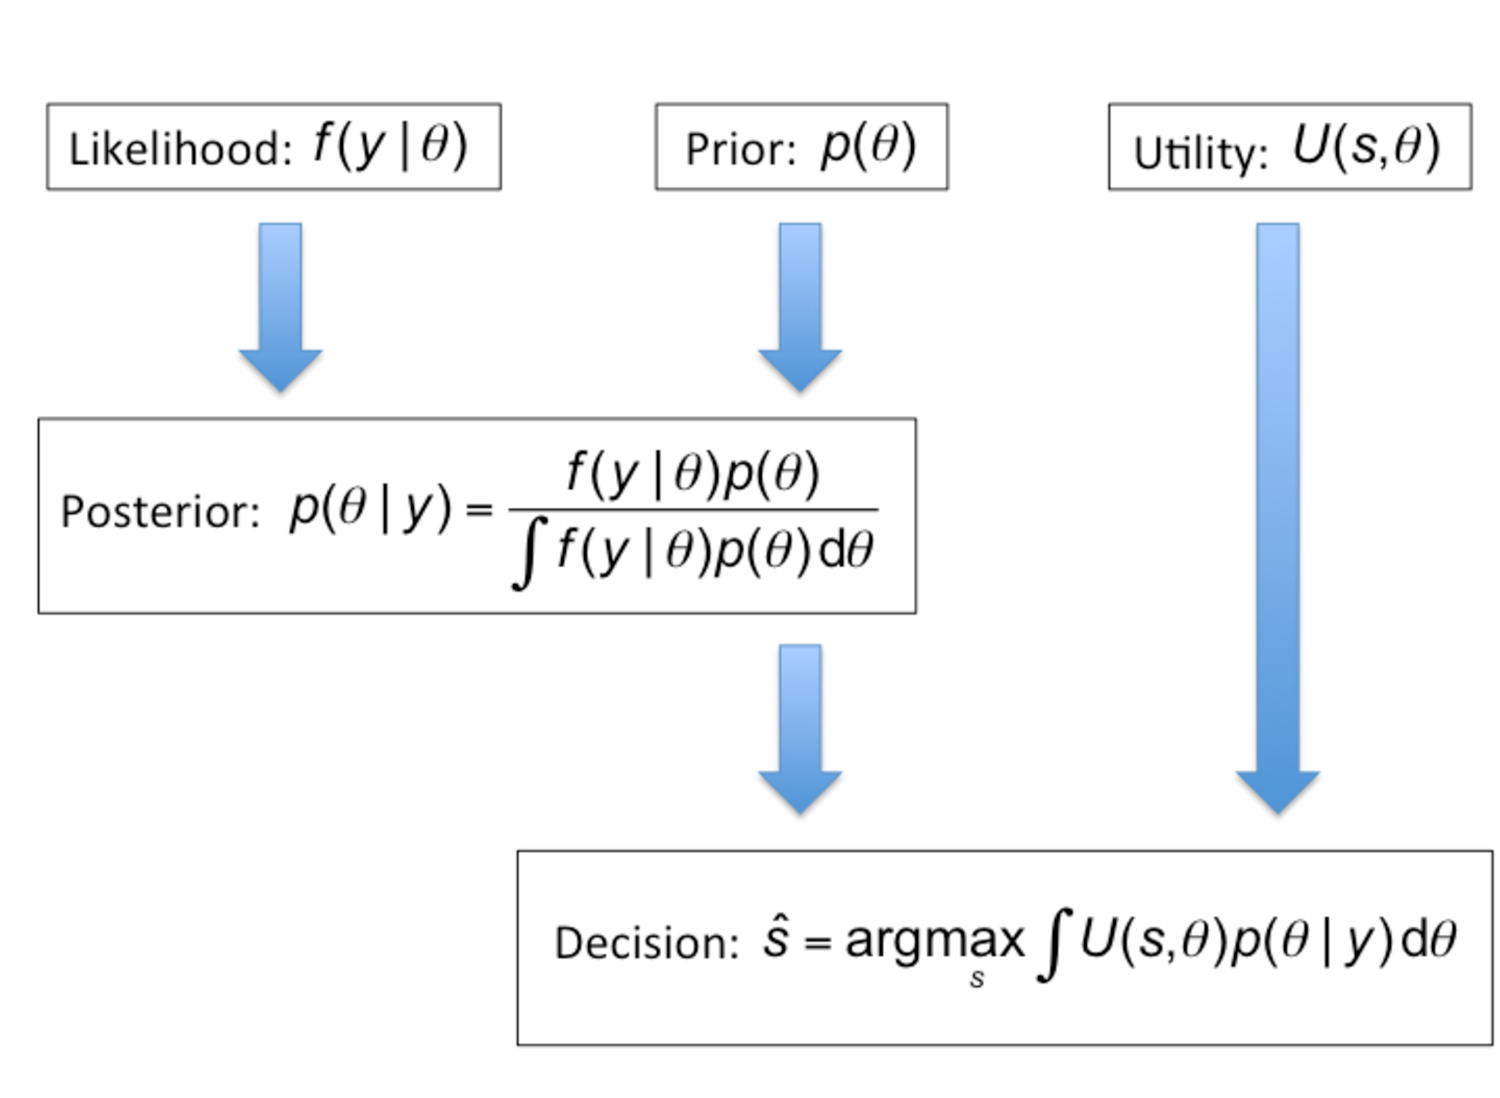
\includegraphics[height=7.0cm,angle=0]{plots/bayes.pdf}
\end{center}
}




\frame{
\sffamily
\frametitle{The Bayesian approach to statistical inference}
\begin{itemize}
\item {\bf Example (estimating the mean of a normal):  }  Assume $y_1, \ldots, y_n$ is an independent and identically distributed sample with $y_i \mid \theta \sim \normal(\theta, 1)$ and assign $\theta$ a Gaussian prior, i.e., $\theta \sim \normal(\mu, \tau^2)$.  Our goal is to provide (Bayesian) point and interval estimates for the unknown parameter $\theta$.

\vspace{1mm}

The first stage in any Bayesian analysis is to determine the posterior density/probability mass function of the parameter(s) of interest (in this case $\theta$).


\end{itemize}
}






\frame{
\sffamily
\frametitle{The Bayesian approach to statistical inference}

\begin{itemize}
\item  {\bf Example (estimating the mean of a normal, cont):}
{\tiny \begin{align*}
p(\bftheta \mid \bfy) =
%
\frac{\left(\frac{1}{2\pi}\right)^{n/2} \exp\left\{ - \frac{1}{2} \sum_{i=1}^{n}(y_i - \theta)^2\right\} \left(\frac{1}{2 \pi \tau^2}\right)^{1/2} \exp\left\{ - \frac{(\theta - \mu)^2}{2\tau^2} \right\}}
%
{\int_{-\infty}^{\infty} \left(\frac{1}{2\pi}\right)^{n/2} \exp\left\{ - \frac{1}{2} \sum_{i=1}^{n}(y_i - \theta)^2\right\} \left(\frac{1}{2 \pi \tau^2}\right)^{1/2} \exp\left\{ - \frac{(\theta - \mu)^2}{2\tau^2} \right\} \dd \theta}
\end{align*}
}

Doing a completion of squares we get
{\tiny \begin{align*}
p(\bftheta \mid \bfy) =  \frac{\exp\left\{  -\frac{1}{2} \left( n + \frac{1}{\tau^2}\right) \left( \theta - \frac{ n\bar{y} + \frac{\mu}{\tau^2}}{n + \frac{1}{\tau^2}} \right)^2 + \frac{1}{2} \frac{ \left(n\bar{y} + \frac{\mu}{\tau^2}\right)^2}{n + \frac{1}{\tau^2}} \right\}}
{\int_{-\infty}^{\infty} \exp\left\{  -\frac{1}{2} \left( n + \frac{1}{\tau^2}\right) \left( \theta - \frac{ n\bar{y} + \frac{\mu}{\tau^2}}{n + \frac{1}{\tau^2}} \right)^2 + \frac{1}{2} \frac{ \left(n\bar{y} + \frac{\mu}{\tau^2}\right)^2}{n + \frac{1}{\tau^2}} \right\} \dd \theta}\end{align*}}

Hence $p(\theta \mid \bfy)$ correspond to a Gaussian distribution with mean $\frac{ n\bar{y} + \frac{\mu}{\tau^2}}{n + \frac{1}{\tau^2}}$ and variance $\left( n + \frac{1}{\tau^2}\right)^{-1}$!
\end{itemize}
}








\frame{
\sffamily
\frametitle{The Bayesian approach to statistical inference}

\begin{itemize}
\item  {\bf Example (estimating the mean of a normal, cont):  }  Now that we have found the posterior distribution, we can use the posterior mean as a point estimator, i.e.,
$$
\tilde{\theta} = \E \left\{ \theta \mid \bfy \right\} = \frac{\int \theta p(\bfy \mid \theta) p(\theta) \dd \theta}{\int p(\bfy \mid \theta) p(\theta) \dd \theta} = \frac{ n\bar{y} + \frac{\mu}{\tau^2}}{n + \frac{1}{\tau^2}} .
$$
Besides being a ``natural'' measure of location of the posterior distribution, the posterior mean can be formally justified as begin the optimal estimator under squared error loss,
\begin{align*}
\E \left\{ \theta \mid \bfy \right\}  &=  \int_{-\infty}^{\infty} \theta p(\theta \mid \bfy) \dd \theta  \\
%
& = \argmax_{\vartheta} \frac{\int (\theta - \vartheta)^2 p(\bfy \mid \theta) p(\theta) \dd \theta}{\int p(\bfy \mid \theta) p(\theta) \dd \theta}
\end{align*}
\end{itemize}
}





\frame{
\sffamily
\frametitle{The Bayesian approach to statistical inference}
\begin{itemize}
\item  {\bf Example (estimating the mean of a normal, cont):  }  Similarly, interval estimates can be obtained by computing highest posterior density intervals (shortest intervals that contain a given amount of posterior probability).  

\vspace{3mm}

In our running example, and for an interval with $1-\alpha$ coverage, this reduces to 
{\small $$
\left(  \frac{ n\bar{y} + \frac{\mu}{\tau^2}}{n + \frac{1}{\tau^2}} - z_{\alpha/2} \left\{ n + \frac{1}{\tau^2}\right\}^{-\frac{1}{2}}
,
\frac{ n\bar{y} + \frac{\mu}{\tau^2}}{n + \frac{1}{\tau^2}} + z_{\alpha/2} \left\{ n + \frac{1}{\tau^2}\right\}^{-\frac{1}{2}} \right) .
$$}

HPD intervals can be justified using utility functions too!
\end{itemize}
}





\frame{
\sffamily
\frametitle{The Bayesian approach to statistical inference}

\begin{itemize}
\item Generally speaking, once the model for the data and the priors/hyperpriors have been selected, performing Bayesian inference involves
\begin{itemize}
\item Computing expectations of functions of the parameters with respect to the posterior distribution.
\item Maximizing the corresponding expected utility functions.
\end{itemize}

\vspace{1mm}

\item We will mostly be focusing on cases where the second step is available in closed form (i.e., we assume simple, ``standard'' utility functions).
\begin{itemize}
\item Historically, the main challenge in using Bayesian methods for real-world problems has been how to do computation beyond simple conjugate models.
\item Numerical integration methods such as Gaussian quadrature scale very poorly (typically not useful if $\mbox{dim}(\bftheta) > 4$).
\end{itemize}
\end{itemize}
}







\frame{
\sffamily
\frametitle{A summary of Bayesian computational methods}
\begin{center}
\hspace{-1.1cm}
\begin{tabular}{lr}
\begin{minipage}{5.6cm}
\centerline{\bf Monte-Carlo integration}
\vspace{0.2cm}
\begin{itemize}
{\small \item Generate samples from $\bftheta^{(1)}, \ldots, \bftheta^{(B)} \sim p(\bftheta \mid \bfy)$.

\item Approximate 
$$
\int h(\bftheta) p(\bftheta \mid \bfy) \dd \bftheta \approx \sum_{b=1}^{B} h \left(\bftheta^{(b)} \right)
$$ 
(WLLN / Ergodic theorem).

\item Examples:  Adaptive Rejection Sampling, Importance Sampling, Markov chain Monte Carlo, Sequential Monte Carlo, Approximate Bayesian Computation.}
\end{itemize}
\end{minipage}
%&
\begin{minipage}{5.6cm}
\centerline{\bf Approximation methods}
\vspace{0.2cm}
\begin{itemize}
{\small \item Find a distribution $q(\bftheta)$ that is analytically tractable and is ``close'' to $p(\bftheta \mid \bfy)$.

\item Approximate
$$
\int h(\bftheta) p(\bftheta \mid \bfy) \dd \bftheta \approx \int h(\bftheta) q(\bftheta) \dd \bftheta
$$ 

\item Examples: Laplace approximations, mean-field variational approximations, integrated nested Laplace
approximations.}
\end{itemize}
\end{minipage}
\end{tabular}
\end{center}
}



\frame{
\sffamily
\frametitle{A summary of Bayesian computational methods}
\begin{itemize}
\item The previous methods are \textit{general}, in the sense that they allow for point and interval estimation, prediction and, in some cases (e.g., reversible jump MCMC, spike-and-slab priorss) variable selection/model comparison.

\item In addition to them, there are methods that are \textit{specific} to either point estimation (typically finding posterior mode) or model selection (typically for computing marginal likelihoods and Bayes factors).
\begin{itemize}
\item Point estimation:  expectation-maximization (yes, it can be used in a Bayesian setting), (stochastic) conjugate gradient, feature selection.

\item Bayes factors:  Harmonic Mean Estimation, Bridge Sampling, the marginal likelihood identity method of Chib, etc.
\end{itemize}


%MCMC methods for computing Bayes factors: a comparative review by: Cong Han, Bradley P. Carlin Journal of the American Statistical Association, Vol. 96 (September 2001), pp. 1122-1132  Key: citeulike:2113706
\end{itemize}
}




\frame{
\sffamily
\frametitle{What this course is about!}
\begin{itemize}
\item As you can see, the literature is extensive, so we will select a small number of topics to discuss:
\begin{itemize}
\item MCMC techniques, including reversible jump, adaptive Monte Carlo, and Hamiltonian methods.

\item Importance sampling and sequential Monte Carlo algorithms for state-space models, but not population Monte Carlo.

\item Variational methods.

\item Laplace approximations and INLA

\end{itemize}

\item Heavy focus on using \texttt{NIMBLE} and other software options to simplify implementation.
\end{itemize}
}







\section{NIMBLE}

\begin{frame}[fragile] 
\sffamily
\frametitle{What is NIMBLE?}

\begin{itemize}
\item A flexible extension of the BUGS and JAGS systems
\item A system for using algorithms on hierarchical statistical models
\item A system for programming algorithms for hierarchical models
\item A partial compiler for math, flow control, and related R code
\end{itemize}

At its most basic level, you can use NIMBLE in place of BUGS or JAGS. But even if you don't use algorithms other than MCMC or take advantage of the NIMBLE programming system, NIMBLE provides additional flexibility on top of BUGS or JAGS:

\begin{itemize}
\item User-defined distributions and functions for use in BUGS code
\item Alternative parameterizations of distributions
\item Flexibility in choosing the samplers to use in an MCMC
\item Ability to arbitrarily block parameters in MCMC sampling
\end{itemize}

\end{frame}

\begin{frame}[fragile] 
\sffamily
\frametitle{The BUGS language}
{\footnotesize

BUGS is a declarative language for graphical (or hierarchical) models.
\begin{itemize}
\item Most programming languages are imperative, which means a series of
commands will be executed in the order they are written.
\item A declarative language like BUGS is more like building a machine before
using it.
\item Each line declares that a component should be plugged into
the machine.
\end{itemize}

The machine in this case is a graphical model (in particular, a
  \textit{directed acyclic graph}).  A \textit{node} (sometimes called
a \textit{vertex}) holds one value, which may be a scalar or a vector.
\textit{Edges} define the relationships between nodes.  A huge variety
of statistical models can be thought of as graphs.  See also:
\begin{itemize}
\item Chapter 5 of the NIMBLE manual -- https://r-nimble.org/documentation
\item the BUGS manual -- http://www.openbugs.net/Manuals/ModelSpecification.html
\end{itemize}
}

\end{frame}

\begin{frame}[fragile] 
\sffamily
\frametitle{Basic regression example in BUGS}

\begin{columns}[T] % align columns
\vspace{5mm}
\begin{column}{.48\textwidth}

\begin{knitrout}\tiny
\definecolor{shadecolor}{rgb}{0.969, 0.969, 0.969}\color{fgcolor}\begin{kframe}
\begin{alltt}
\hlstd{regrCode} \hlkwb{<-} \hlkwd{nimbleCode}\hlstd{(\{}
    \hlcom{## priors}
    \hlstd{intcpt} \hlopt{~} \hlkwd{dnorm}\hlstd{(}\hlnum{0}\hlstd{,} \hlkwc{sd} \hlstd{=} \hlnum{1000}\hlstd{)}
    \hlstd{slope} \hlopt{~} \hlkwd{dnorm}\hlstd{(}\hlnum{0}\hlstd{,} \hlkwc{sd} \hlstd{=} \hlnum{1000}\hlstd{)}
    \hlcom{## Gelman (2006) recommended prior:}
    \hlstd{sigma} \hlopt{~} \hlkwd{dunif}\hlstd{(}\hlnum{0}\hlstd{,} \hlnum{100}\hlstd{)}

    \hlkwa{for}\hlstd{(i} \hlkwa{in} \hlnum{1}\hlopt{:}\hlnum{4}\hlstd{) \{}
        \hlcom{## linear predictor (deterministic node)}
        \hlstd{pred_y[i]} \hlkwb{<-} \hlstd{intcpt} \hlopt{+} \hlstd{slope} \hlopt{*} \hlstd{x[i]}
        \hlcom{## likelihood }
        \hlstd{y[i]} \hlopt{~} \hlkwd{dnorm}\hlstd{(pred_y[i],} \hlkwc{sd} \hlstd{= sigma)}
    \hlstd{\}}
\hlstd{\})}
\end{alltt}
\end{kframe}
\end{knitrout}

\end{column}%

\begin{column}{.48\textwidth}
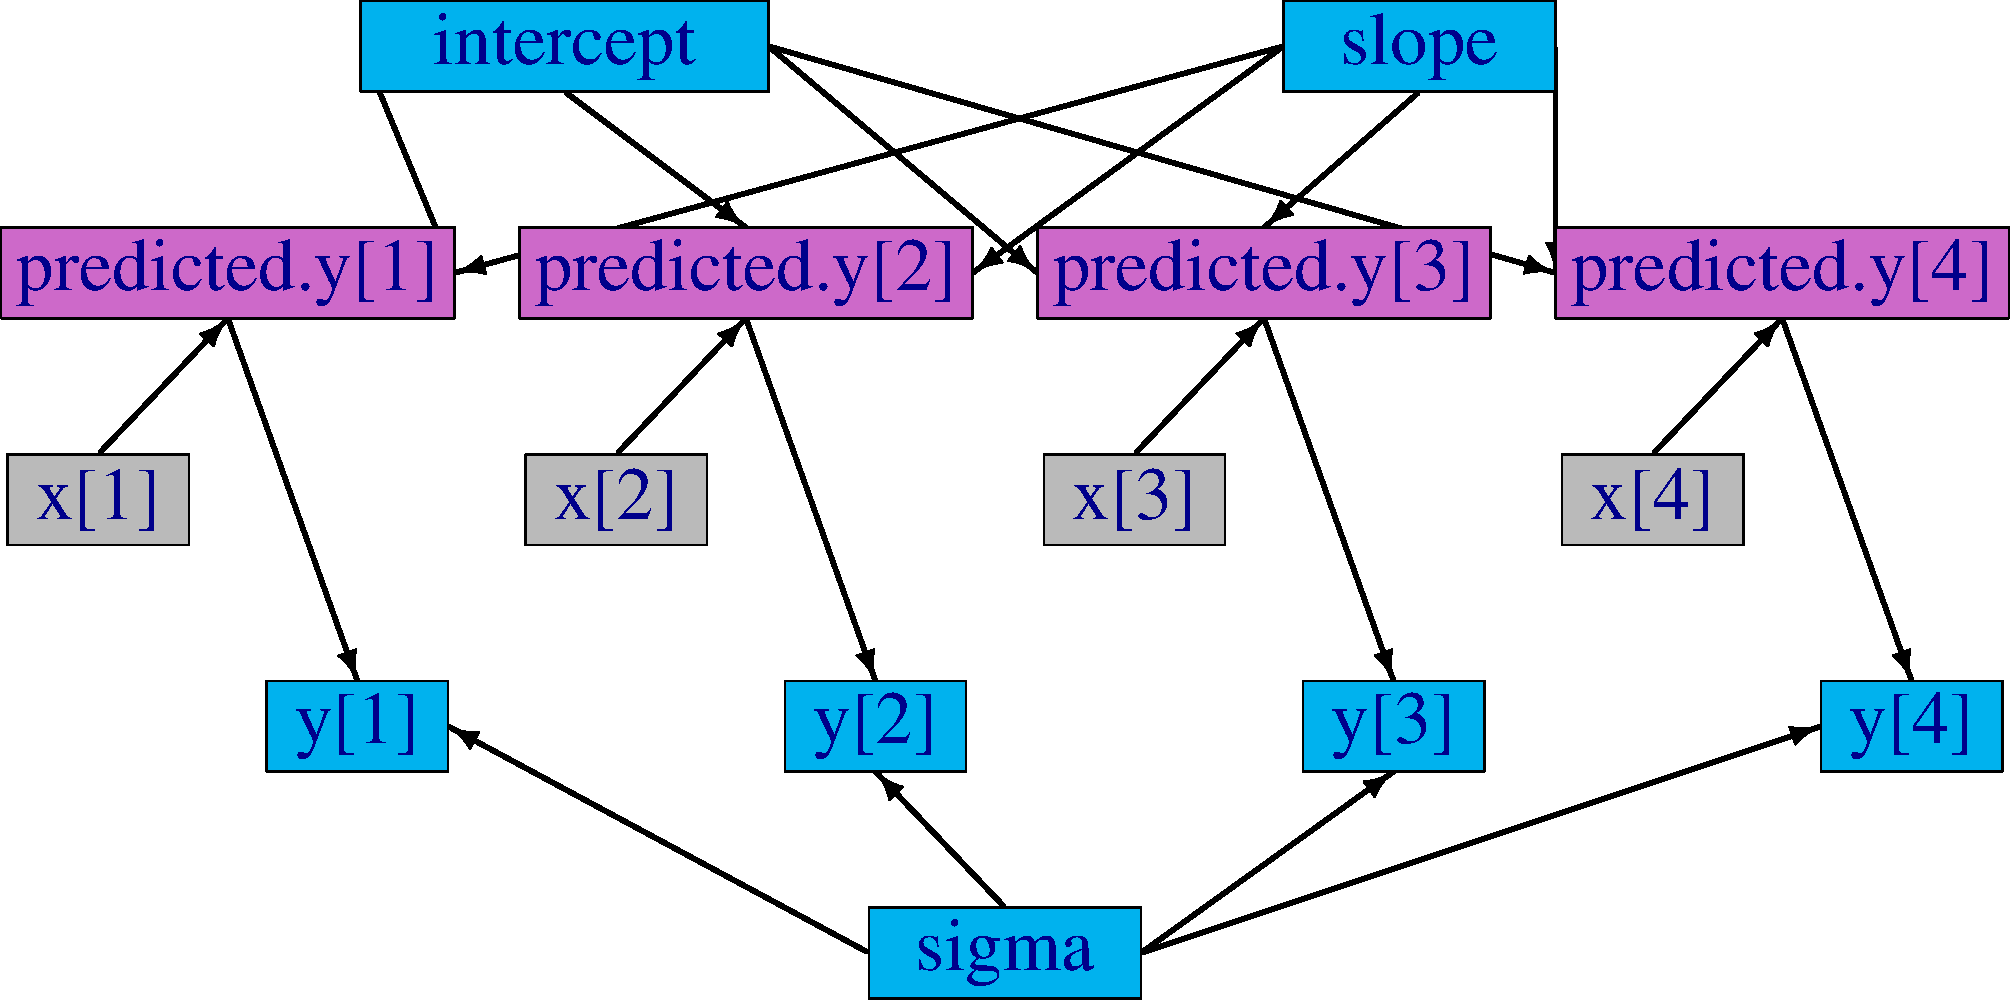
\includegraphics[width=2.2in]{plots/linearRegressionGraph-crop.pdf}
\end{column}%
\end{columns}

Stochastic relationships are declared with $\sim$
and deterministic relationships with \texttt{<-}.

See Chapter 5 of the NIMBLE manual for available distributions, default and alternative parameterizations, and functions.

We don't actually need the \texttt{pred\_y} line of code; could have:
\begin{knitrout}\scriptsize
\definecolor{shadecolor}{rgb}{0.969, 0.969, 0.969}\color{fgcolor}\begin{kframe}
\begin{alltt}
\hlstd{y[i]} \hlopt{~} \hlkwd{dnorm}\hlstd{(intcpt} \hlopt{+} \hlstd{slope} \hlopt{*} \hlstd{x[i],} \hlkwc{sd} \hlstd{= sigma)}
\end{alltt}
\end{kframe}
\end{knitrout}

\end{frame}

\begin{frame}[fragile] 
\sffamily
\frametitle{GLMM example}

{\footnotesize
\begin{itemize}
\item The litters model from the original 1995 BUGS software has data on rat pup survival for pups in 16 litters in each of two groups.  Survival within a litter is governed by a survival probability specific to the litter.
\item Probabilities for each group are treated as being exchangeable, coming from a common beta distribution to induce shrinkage. 

\begin{knitrout}\tiny
\definecolor{shadecolor}{rgb}{0.969, 0.969, 0.969}\color{fgcolor}\begin{kframe}
\begin{alltt}
\hlstd{glmmCode} \hlkwb{<-} \hlkwd{nimbleCode}\hlstd{(\{}
  \hlkwa{for} \hlstd{(i} \hlkwa{in} \hlnum{1}\hlopt{:}\hlstd{G) \{}
      \hlcom{## priors for hyperparameters (from original example, not necessarily recommended)}
     \hlstd{a[i]} \hlopt{~} \hlkwd{dgamma}\hlstd{(}\hlnum{1}\hlstd{,} \hlnum{.001}\hlstd{)}
     \hlstd{b[i]} \hlopt{~} \hlkwd{dgamma}\hlstd{(}\hlnum{1}\hlstd{,} \hlnum{.001}\hlstd{)}
     \hlkwa{for} \hlstd{(j} \hlkwa{in} \hlnum{1}\hlopt{:}\hlstd{N) \{}
        \hlcom{## random effects ('latent process')}
        \hlstd{p[i,j]} \hlopt{~} \hlkwd{dbeta}\hlstd{(a[i], b[i])}
        \hlcom{## likelihood }
        \hlstd{r[i,j]} \hlopt{~} \hlkwd{dbin}\hlstd{(p[i,j], n[i,j])}
     \hlstd{\}}
   \hlstd{\}          \})}
\end{alltt}
\end{kframe}
\end{knitrout}

\item This is a GLMM structure (albeit without any explicit fixed effects, though they are implicit in the grouping).
\item We could write an alternative version with a logistic link, normal random effects, and a group-based offset.
\end{itemize}
}
\end{frame}

\begin{frame}[fragile] 
\sffamily
\frametitle{Models in NIMBLE}
{\scriptsize
In WinBUGS and JAGS, the model and its MCMC are tied together. NIMBLE's approach is to separate the model and the algorithm(s) used with a model. This allows for:

\begin{itemize}
\item use of the model for other purposes, such as simulating from it in a simulation study,
\item customization of MCMCs for a given model (e.g., changing samplers and blocking),
\item use of other algorithms (e.g., SMC, MCEM, eventually INLA, VB, etc.) on a model, and
\item programming new algorithms for use with any model.
\end{itemize}

Let's create a model from the BUGS code.
}
\begin{knitrout}\scriptsize
\definecolor{shadecolor}{rgb}{0.969, 0.969, 0.969}\color{fgcolor}\begin{kframe}
\begin{alltt}
\hlstd{consts} \hlkwb{<-} \hlkwd{list}\hlstd{(}\hlkwc{G} \hlstd{=} \hlnum{2}\hlstd{,} \hlkwc{N} \hlstd{=} \hlnum{16}\hlstd{,}
     \hlkwc{n} \hlstd{=} \hlkwd{matrix}\hlstd{(}\hlkwd{c}\hlstd{(}\hlnum{13}\hlstd{,}\hlnum{12}\hlstd{,}\hlnum{12}\hlstd{,}\hlnum{11}\hlstd{,}\hlnum{9}\hlstd{,}\hlnum{10}\hlstd{,}\hlnum{9}\hlstd{,}\hlnum{9}\hlstd{,}\hlnum{8}\hlstd{,}\hlnum{11}\hlstd{,}\hlnum{8}\hlstd{,}\hlnum{10}\hlstd{,}\hlnum{13}\hlstd{,}\hlnum{10}\hlstd{,}\hlnum{12}\hlstd{,}\hlnum{9}\hlstd{,}
           \hlnum{10}\hlstd{,}\hlnum{9}\hlstd{,}\hlnum{10}\hlstd{,}\hlnum{5}\hlstd{,}\hlnum{9}\hlstd{,}\hlnum{9}\hlstd{,}\hlnum{13}\hlstd{,}\hlnum{7}\hlstd{,}\hlnum{5}\hlstd{,}\hlnum{10}\hlstd{,}\hlnum{7}\hlstd{,}\hlnum{6}\hlstd{,}\hlnum{10}\hlstd{,}\hlnum{10}\hlstd{,}\hlnum{10}\hlstd{,}\hlnum{7}\hlstd{),} \hlkwc{nrow} \hlstd{=} \hlnum{2}\hlstd{))}
\hlstd{data} \hlkwb{=} \hlkwd{list}\hlstd{(}\hlkwc{r} \hlstd{=} \hlkwd{matrix}\hlstd{(}\hlkwd{c}\hlstd{(}\hlnum{13}\hlstd{,}\hlnum{12}\hlstd{,}\hlnum{12}\hlstd{,}\hlnum{11}\hlstd{,}\hlnum{9}\hlstd{,}\hlnum{10}\hlstd{,}\hlnum{9}\hlstd{,}\hlnum{9}\hlstd{,}\hlnum{8}\hlstd{,}\hlnum{10}\hlstd{,}\hlnum{8}\hlstd{,}\hlnum{9}\hlstd{,} \hlnum{12}\hlstd{,}\hlnum{9}\hlstd{,}\hlnum{11}\hlstd{,}\hlnum{8}\hlstd{,}\hlnum{9}\hlstd{,}\hlnum{8}\hlstd{,}\hlnum{9}\hlstd{,}
                         \hlnum{4}\hlstd{,}\hlnum{8}\hlstd{,}\hlnum{7}\hlstd{,}\hlnum{11}\hlstd{,}\hlnum{4}\hlstd{,}\hlnum{4}\hlstd{,}\hlnum{5}\hlstd{,}\hlnum{5}\hlstd{,}\hlnum{3}\hlstd{,}\hlnum{7}\hlstd{,}\hlnum{3}\hlstd{,}\hlnum{7}\hlstd{,}\hlnum{0}\hlstd{),} \hlkwc{nrow} \hlstd{=} \hlnum{2}\hlstd{))}
\hlstd{inits} \hlkwb{<-} \hlkwd{list}\hlstd{(}\hlkwc{a} \hlstd{=} \hlkwd{c}\hlstd{(}\hlnum{2}\hlstd{,} \hlnum{2}\hlstd{),} \hlkwc{b} \hlstd{=} \hlkwd{c}\hlstd{(}\hlnum{2}\hlstd{,} \hlnum{2}\hlstd{))}
\hlcom{## create a model object that can be used and modified}
\hlstd{model} \hlkwb{<-} \hlkwd{nimbleModel}\hlstd{(glmmCode,} \hlkwc{constants} \hlstd{= consts,} \hlkwc{data} \hlstd{= data,} \hlkwc{inits} \hlstd{= inits)}
\end{alltt}
\end{kframe}
\end{knitrout}

\end{frame}

\begin{frame}[fragile] 
\sffamily
\frametitle{Data vs. constants}

\begin{itemize}
\item data: observations that contribute to the likelihood (and in some cases predictors/covariates)
\item constants: values that never change and must include any indexing limits (e.g., \texttt{n} in \texttt{for(i in 1:n)})
\item inits: initial values for parameters (or in some cases predictors/covariates)
\end{itemize}

\end{frame}


\begin{frame}[fragile] 
\sffamily
\frametitle{'Operating' the model}
{\small
You can move values into and out of the model, simulate from the priors, and calculate prior densities ('logProbs'), as well as examining relationships in the model.

\begin{knitrout}\scriptsize
\definecolor{shadecolor}{rgb}{0.969, 0.969, 0.969}\color{fgcolor}\begin{kframe}
\begin{alltt}
\hlstd{model}\hlopt{$}\hlstd{p}
\hlstd{model}\hlopt{$}\hlkwd{simulate}\hlstd{(}\hlstr{'p'}\hlstd{)}
\hlstd{model}\hlopt{$}\hlstd{p}
\hlstd{model}\hlopt{$}\hlstd{p} \hlkwb{<-} \hlkwd{matrix}\hlstd{(}\hlnum{0.5}\hlstd{, consts}\hlopt{$}\hlstd{G, consts}\hlopt{$}\hlstd{N)}
\hlcom{## IMPORTANT - don't assume you know what child nodes do or}
\hlcom{## don't need to be updated once you've changed values in the model:}
\hlstd{model}\hlopt{$}\hlkwd{calculate}\hlstd{(model}\hlopt{$}\hlkwd{getDependencies}\hlstd{(}\hlstr{'p'}\hlstd{))}
\hlstd{model}\hlopt{$}\hlkwd{calculate}\hlstd{(}\hlstr{'r'}\hlstd{)}

\hlcom{## plot(model$graph)}
\hlstd{model}\hlopt{$}\hlkwd{getDependencies}\hlstd{(}\hlstr{'a[1]'}\hlstd{)}
\hlstd{model}\hlopt{$}\hlkwd{getDependencies}\hlstd{(}\hlstr{'a[1]'}\hlstd{,} \hlkwc{determOnly} \hlstd{=} \hlnum{TRUE}\hlstd{)}
\hlstd{model}\hlopt{$}\hlkwd{getDependencies}\hlstd{(}\hlstr{'a[1]'}\hlstd{,} \hlkwc{dataOnly} \hlstd{=} \hlnum{TRUE}\hlstd{)}
\hlstd{model}\hlopt{$}\hlkwd{getDependencies}\hlstd{(}\hlstr{'a[1]'}\hlstd{,} \hlkwc{dataOnly} \hlstd{=} \hlnum{TRUE}\hlstd{,} \hlkwc{downstream} \hlstd{=} \hlnum{TRUE}\hlstd{)}
\end{alltt}
\end{kframe}
\end{knitrout}

}
\end{frame}






\section{MCMC}


\frame{
\sffamily
\frametitle{Why simulation based methods:  A motivating example}
\begin{itemize}
\item  To illustrate the power of simulation methods, consider the problem of estimating the diagnostic power of a medical test, defined as the probability of a positive result in the test for a diseased individual.
$$
\eta = \Pr\left( D \mid T \right) .
$$

\item $\eta$ is not directly observable.  However, we can easily obtain data on the prevalence $\theta$, the false positive rate $\alpha$ and the false negative rate $\beta$,
\begin{align*}
\theta &= \Pr(D) , &
\alpha & = \Pr \left( T \mid \bar{D} \right)  , &
\beta & = \Pr \left( \bar{T} \mid D \right) ,
\end{align*}
by sampling individuals from the general population, the population of healthy individuals, and the population of diseased individuals, respectively.
\end{itemize}
}




\frame{
\sffamily
\frametitle{A motivating example}
\begin{itemize}
\item Note that $\eta$ is related to $\theta$, $\alpha$ and $\beta$ by the formula:
$$
\eta(\theta, \alpha, \beta) = \frac{(1-\beta) \theta}{(1-\beta) \theta + \alpha (1-\theta)}  .
$$
(This is just Bayes theorem!)

\item {\bf Statistical model: } Assuming that individuals are sampled at random from the corresponding populations 
\begin{align*}
x_1 &= \left\{ \mbox{\parbox[c][][c]{6cm}{\# of diseased individuals in a sample of size $n_1$ of the general population}} \right\}  \sim \Bin(n_1, \theta)  , \\
x_2 &= \left\{\mbox{\parbox[c][][c]{6cm}{\# of positive individuals in a sample of size $n_2$ of healthy individuals}}\right\} \sim \Bin(n_2, \alpha) , \\
x_3 &= \left\{\mbox{\parbox[c][][c]{6cm}{\# of positive individuals in a sample of size $n_3$ of diseased individuals}}\right\} \sim \Bin(n_3, 1-\beta)  .
\end{align*}

\end{itemize}
}



\frame{
\sffamily
\frametitle{A motivating example}
\begin{itemize}
\item A frequentist approach:
\begin{itemize}
\item {\bf Point estimation:  }  The MLEs for $\theta$, $\alpha$ and $\beta$ are
\begin{align*}
\hat{\theta} &= \frac{x_1}{n_1} ,   &  \hat{\alpha} &= \frac{x_2}{n_2} ,   &  \hat{\beta} &= 1 - \frac{x_3}{n_3} .
\end{align*}
Hence, the MLE of $\eta$ is simply $\hat{\eta} = \frac{(1-\hat{\beta}) \hat{\theta}}{(1-\hat{\beta}) \hat{\theta} + \hat{\alpha} (1-\hat{\theta})}$.
\vspace{1mm}
\item {\bf Interval estimation:  }  Finding a pivot for $\eta$ is hard.  However, an asymptotic approximate interval can be constructed using the Delta method
\begin{align*}
\Var(\hat{\eta}) \approx  
%
\left[ \left. \nabla \eta(\theta,\alpha,\beta) \right|_{(\hat{\theta},\hat{\alpha},\hat{\beta})} \right]^T 
\bfSigma \left[ \left. \nabla \eta(\theta,\alpha,\beta) \right|_{(\hat{\theta},\hat{\alpha},\hat{\beta})} \right]
\end{align*}
where $\bfSigma = \diag\left\{ \Var(\hat{\theta}), \Var(\hat{\alpha}), \Var(\hat{\beta})  \right\}$.

\vspace{2mm}

For small samples, parametric bootstrap could be used (which is a simulation-based computational tool common in frequentist statistics).
\end{itemize}
\end{itemize}
}



\frame{
\sffamily
\frametitle{A motivating example}
\begin{itemize}
\item A frequentist approach (cont):
\begin{itemize}
\item {\bf Interval estimation (cont):  }  Parametric bootstrap:  Once $\hat{\theta}$,$\hat{\alpha}$ and $\hat{\beta}$ have been computed, repeat the following steps for $b=1,\ldots,B$ where $B$ is ``large'':
\begin{enumerate}
\item Sample imaginary samples $x_1^{(b)} \sim \Bin(n_1, \hat{\theta})$, $x_2^{(b)} \sim \Bin(n_2, \hat{\alpha})$ and $x_3^{(b)} \sim \Bin(n_3, 1 - \hat{\beta})$.

\item Compute $\tilde{\theta}^{(b)} = \frac{x_1^{(b)}}{n_1}$, $\tilde{\alpha}^{(b)} = \frac{x_2^{(b)}}{n_2}$ and $\tilde{\beta}^{(b)} = 1-\frac{x_3^{(b)}}{n_3}$ and let $\tilde{\eta}^{(b)} = \frac{(1-\tilde{\beta}^{(b)}) \tilde{\theta}^{(b)}}{(1-\tilde{\beta}^{(b)}) \tilde{\theta}^{(b)} + \tilde{\alpha}^{(b)} (1-\tilde{\theta}^{(b)})}$.
\end{enumerate}

\vspace{2mm}

Then, an $\epsilon$-coverage confidence interval for $\eta$ is obtained by computing the $\epsilon/2$ and $1-\epsilon/2$ quantiles of the sample $\tilde{\beta}^{(1)} , \ldots, \tilde{\beta}^{(B)}$.
\end{itemize}
\end{itemize}
}



\frame{
\sffamily
\frametitle{A motivating example}
\begin{itemize}
\item A Bayesian approach:
\begin{itemize}
\item {\bf Priors:  }  Natural non-informative priors for this problem are $\theta \sim \bet\left( \frac{1}{2} , \frac{1}{2}\right)$, $\alpha \sim \bet\left( \frac{1}{2} , \frac{1}{2}\right)$ and $\beta \sim \bet\left( \frac{1}{2} , \frac{1}{2}\right)$.

\vspace{2mm}

\item {\bf Posteriors:  }  Because of independence and conjugacy we have 
{\scriptsize \begin{multline*}
p(\theta, \alpha, \beta \mid x_1, x_2, x_3) = \bet \left( \theta \mid \frac{1}{2} + x_1 , \frac{1}{2} + n_1 - x_1 \right) \\
%
\bet \left( \alpha \mid \frac{1}{2} + x_2 , \frac{1}{2} + n_2 - x_2 \right) 
%
\bet \left( \beta \mid \frac{1}{2} + n_3 - x_3 , \frac{1}{2} + x_3 \right)
\end{multline*}}
Since $\eta$ is a function of $(\theta,\alpha,\beta)$, its posterior can be obtained through transformations.  However, in this case, this is extremely messy ... Try it yourself.
\end{itemize}
\end{itemize}
}



\frame{
\sffamily
\frametitle{A motivating example}
\begin{itemize}
\item A Bayesian approach:
\begin{itemize}
\item {\bf Using a simulation-based approach:  }    Instead of trying to find a closed-form expression for $p(\eta \mid x_1, x_2, x_3)$, sample!

\begin{enumerate}
\item For $b=1,\ldots,B$ generate $\theta^{(b)} \sim \bet \left( \frac{1}{2} + x_1 , \frac{1}{2} + n_1 - x_1 \right)$, $\alpha^{(b)} \sim \bet \left( \frac{1}{2} + x_2 , \frac{1}{2} + n_2 - x_2 \right)$ and $\beta^{(b)} \sim \bet \left( \frac{1}{2} + n_3 - x_3 , \frac{1}{2} + x_3 \right)$.

\item For $b=1,\ldots,B$ let $\eta^{(b)} = \frac{(1-\beta^{(b)}) \theta^{(b)}}{(1-\beta^{(b)}) \theta^{(b)} + \alpha^{(b)} (1-\theta^{(b)})}$.
\end{enumerate}

\item Density $\Rightarrow$ histogram or a kernel density estimator.

\item Posterior mean or median $\Rightarrow$ Empirical ean or median.

\item An $\epsilon$-probability credible interval $\Rightarrow$ $\epsilon/2$ and $1-\epsilon/2$ quantiles of $\eta^{(1)}, \ldots, \eta^{(B)}$.
\end{itemize}
\end{itemize}
\begin{center}
Let's run the scripts in the file \texttt{simulationmotivation.R}.
\end{center}
}



\frame{
\sffamily
\frametitle{Motivation for MCMC algorithms}
\begin{itemize}
\item Direct sampling like in the previous example is not feasible for many models of interest, particularly those involving large numbers of parameters.

\item In \textit{optimization} problems, this ``curse of dimensionality'' is dealt with by using conditional gradient algorithms.
\end{itemize}
\vspace{-8mm}
\begin{center}
\begin{tabular}{lr}
\begin{minipage}{5.2cm}
Conditional gradient algorithms repeatedly optimizes along one single dimension while keeping the value of the rest fixed.
\end{minipage}
&
\begin{minipage}{5.2cm}
\begin{center}
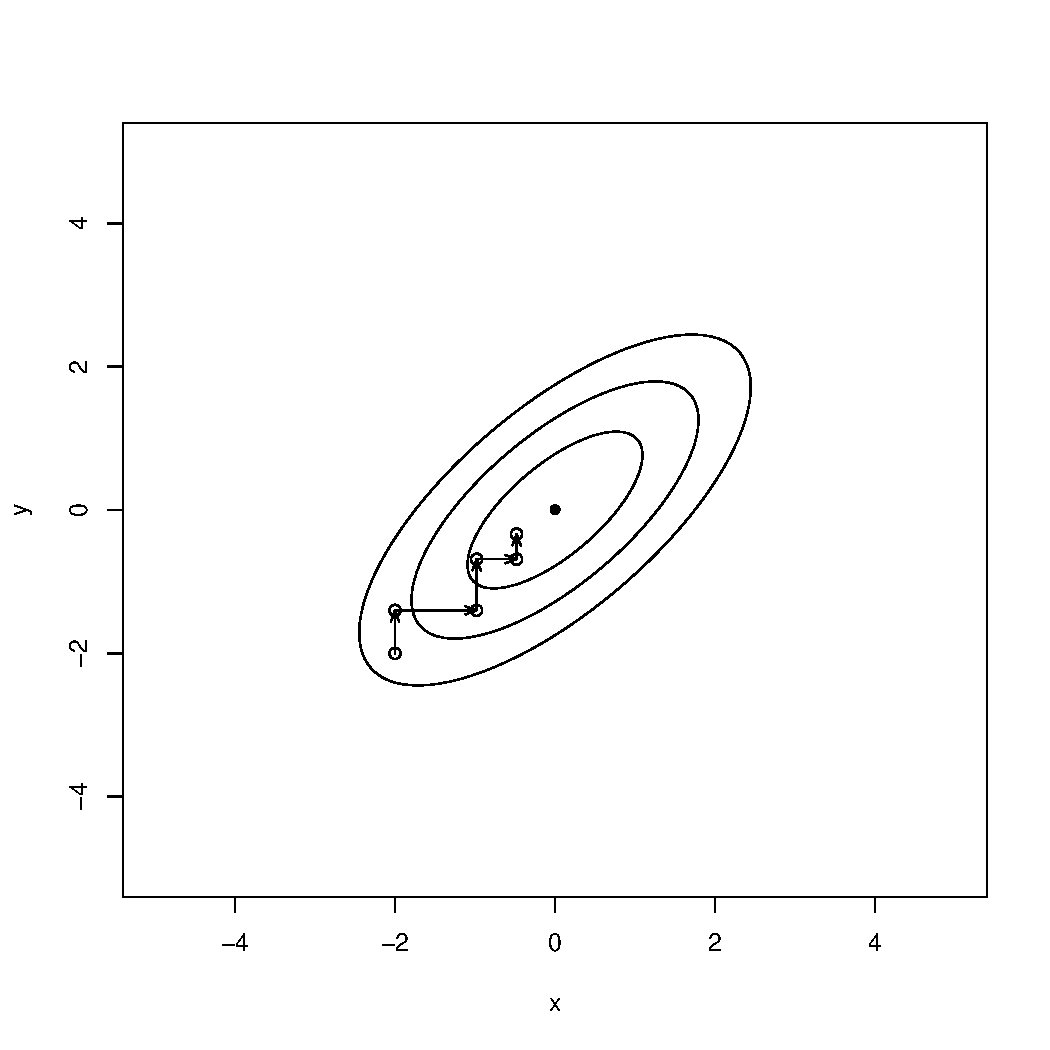
\includegraphics[height=5.4cm,angle=0]{plots/rconjugategradient.pdf}\\
\end{center}
\end{minipage}
\end{tabular}
\end{center}
}






\frame{
\sffamily
\frametitle{Motivation for MCMC algorithms}
\begin{itemize}
\item {\bf Example (Gaussian distributions with unknown mean and variance):}  Assume that data $y_1, \ldots, y_n$ are independent and identically distributed with $y_i \mid \theta, \sigma^2 \sim \normal(\theta, \sigma^2)$ and that we use independent priors $\theta \sim \normal (\mu, \tau^2)$ and $\sigma^2 \sim \IGam(a, c)$.  After some algebra the posterior distribution reduces to
\begin{multline*}
p(\theta, \sigma^2 \mid y_1, \ldots, y_n) \propto \left(\frac{1}{\sigma^2}\right)^{\frac{n}{2} + a + 1} \\
%
\exp\left\{ -\frac{n\theta^2 - 2n\theta \bar{y} + \sum_{i=1}^{n} y_i^2 + 2c}{2\sigma^2} - \frac{\theta^2 - 2\theta\mu + \mu^2}{2\tau^2}   \right\} .
\end{multline*}
This posterior is intractable (by which I mean, computing means/variances and cumulative probabilities is difficult).

\end{itemize}
}





\frame{
\sffamily
\frametitle{Motivation for MCMC algorithms}
\begin{itemize}
\item {\bf Example (Gaussian distributions with unknown mean and variance, cont):}  However, we can try to find the posterior mode (which would provide us with a point estimate for $(\theta, \sigma^2)$ in the same spirit as the MLE) using iterative conditional modes.  

\vspace{1mm}

Starting with some initial guess $\left(\theta^{(0)}, \sigma^{2(0)} \right)$ (such as $\left(\theta^{(0)}, \sigma^{2(0)} \right) = \left( \bar{y}, \Var(y) \right)$), iterate through:
\begin{enumerate}
\item Set $\theta^{(b)} = \frac{\frac{n \bar{y}}{\sigma^{2(b-1)}} + \frac{\mu}{\tau^2}}{\frac{n}{\sigma^{2(b-1)}} + \frac{1}{\tau^2}}$.
\item Set $\sigma^{2(b)} = \frac{2 b + \sum_{i=1}^{n}\left(y_i - \theta^{(b)} \right)^2}{n + 2a + 2}$.
\end{enumerate}
The algorithm is stopped when the value of the posterior ``does not change'' from one iteration to the next.

\vspace{1mm}

See the file \texttt{simpleconjugategradient.R}.
\end{itemize}
}






\frame{
\sffamily
\frametitle{Motivation for MCMC algorithms}
\begin{itemize}
\item Iterative conditional modes only gives us a point estimator and does not allow for full exploration of the posterior distribution (e.g., to compute credible intervals).  

\item What would be an equivalent idea for \textit{sampling} from a distribution $p(\bftheta)$ with $\bftheta = (\theta_1, \ldots, \theta_p)$?
\begin{itemize}
\item If we consider a single dimension at a time we end up working with the \textit{full conditional} $p(\theta_i \mid \theta_1, \ldots, \theta_{i-1}, \theta_{i+1}, \ldots, \theta_{p})$.
\item Because we are trying to sample, maybe we can get a new value of $\theta_i$ by simulating from $p(\theta_i \mid \theta_1, \ldots, \theta_{i-1}, \theta_{i+1}, \ldots, \theta_{p})$ instead of by maximizing it.
\end{itemize}

\item Does this work?
\begin{itemize}
\item Generally speaking, the answer is yes, this is the Gibbs sampler!
\end{itemize}

\end{itemize}
}



\frame{
\sffamily
\frametitle{Motivation for MCMC algorithms}
\begin{itemize}
\item {\bf Example (Gaussian distributions with unknown mean and variance, cont):}  We do not know how to sample directly from the posterior distribution.  However:
\begin{align*}
\theta \mid \sigma^2, y_1, \ldots, y_n \sim \normal \left( 
\frac{\frac{n \bar{y}}{\sigma^2} + \frac{\mu}{\tau^2}}{\frac{n}{\sigma^2} + \frac{1}{\tau^2}}  ,
%
\frac{1}{\frac{n}{\sigma^2} + \frac{1}{\tau^2}}
\right) ,
\end{align*}
and
\begin{align*}
\sigma^2 \mid \theta, y_1, \ldots, y_n \sim \IGam \left( 
a + \frac{n}{2} ,
%
c + \frac{1}{2} \sum_{i=1}^{n} (y_i -\theta)^2 
\right) .
\end{align*}
\end{itemize}
(To find these full conditionals, just drop from the posterior all the -- multiplicative --  terms that do not involve the parameter of interest, and then try to recognize what is left as the kernel of a known distribution.) 
}


\frame{
\sffamily
\frametitle{Motivation for MCMC algorithms}
\begin{itemize}
\item {\bf Example (Gaussian distributions with unknown mean and variance, cont):}  The iterative algorithm looks like this

\begin{enumerate}
\item Initialize $\tilde{\theta}^{(0)}$ and $\tilde{\sigma}^{2(0)}$.
\item For $b=1,\ldots, B$ repeat
\begin{enumerate}
\item Sample $\tilde{\theta}^{(b)} \sim \normal \left( 
\frac{\frac{n \bar{y}}{\tilde{\sigma}^{2(b-1)}} + \frac{\mu}{\tau^2}}{\frac{n}{\tilde{\sigma}^{2(b-1)}} + \frac{1}{\tau^2}}  ,
%
\frac{1}{\frac{n}{\tilde{\sigma}^{2(b-1)}} + \frac{1}{\tau^2}}
\right)$.
\item Sample $\tilde{\sigma}^{2(b)} \sim  \IGam \left( 
a + \frac{n}{2} ,
%
c + \frac{1}{2} \sum_{i=1}^{n} \{y_i -\tilde{\theta}^{(b)}\}^2 
\right)$.
\end{enumerate}
\end{enumerate}

\vspace{1mm}

An example of this implementation in R is available in the file \texttt{simpleGibbs.R}.
\begin{itemize}
\item Run the algorithm first with $\theta^{(0)} = 98$ and $\sigma^{2(0)} = 1$ and then with $\theta^{(0)} = 0$ and $\sigma^{2(0)} = 1600$.  What differences do you see in the trace plots?
\end{itemize}
\end{itemize}
}



\frame{
\sffamily
\frametitle{Motivation for MCMC algorithms}
\begin{itemize}
\item A couple of things to keep in mind:

\begin{itemize}
\item Unlike iterative conditional modes, we care about all numbers generated by the sampler, not only about the last one (we are trying to explore the whole distribution, not just find where the mean/median/mode is).

\item Note that when the initial values are too far from where most of the mass of the posterior is located (as in the second set of initial values), the first few samples are clearly wrong and can seriously bias the results. Hence they need to be discarded.
\end{itemize}

\item Because in the Gibbs sampler we are dealing with a distribution, we need to think about convergence in the probabilistic sense (almost surely/distribution/probability) rather than in terms of convergence in the sense we talk in analysis.
\end{itemize}
}



\frame{
\sffamily
\frametitle{Motivation for MCMC algorithms}
\begin{itemize}
\item Because the value of each pair $\left(\theta^{(b)}, \sigma^{2(b)}\right)$ depends on the value of $\left(\theta^{(b-1)}, \sigma^{2(b-1)}\right)$ (but NOT on $\left(\theta^{(b-2)}, \sigma^{2(b-2)}\right) , \ldots , \left(\theta^{(1)}, \sigma^{2(1)}\right)$) we are actually dealing with a Markov chain!

\item The Gibbs sampler is but one example of a class of algorithms that attempt to construct Markov chains whose limiting distributions correspond to the posterior distribution of interest, and then iterate the 
chain to generate (dependent) samples that can be used to approximate any integral of interest.  Hence the name of Markov chain Monte Carlo methods!

\item For a history of MCMC algorithms, see \cite{robert2011short}.
\end{itemize}
}



\frame{
\sffamily
\frametitle{A brief review of Markov chains}
\begin{itemize}
\item A \textit{Markov chain} is a sequence of random variables $X_1, X_2, X_3 \ldots$ defined on a common probability space $(\Omega, \mathcal{B})$ such that the distribution of $X_t$ given $X_{t-1}, \ldots, X_{1}$ depends only on $X_{t-1}$, i.e., 
\begin{multline*}
\Pr(X_t \in A \mid X_{t-1} = x_{t-1}, \ldots, X_1 = x_1) = \\
%
\Pr(X_t \in A \mid X_{t-1} = x_{t-1})
$$
\end{multline*}

\item It is convenient to think of $t$ as representing time.
\end{itemize}
}



\frame{
\sffamily
\frametitle{A brief review of Markov chains}
\begin{itemize}
\item Markov chains are defined in terms of \textit{transition kernels}.

\vspace{2mm}

\item A \textit{transition kernel} is a function $K$ defined on $\Omega \times \mathcal{B}$ such that
\begin{enumerate}
\item For all $x \in \Omega$, $K(x,\cdot)$ is a probability measure.
\item For all $A \in \mathcal{B}$, $K(\cdot, A)$ is measurable.
\end{enumerate}

\vspace{2mm}

\item We will focus on \textit{time-homogeneous chains} where the transition kernel is the same for all $t$.
\begin{itemize}
\item When $\Omega$ is countable the transition kernel is a matrix such that $[\bfP ]_{x,y} = \Pr(X_t= y \mid X_{t-1} = x)$ where $x,y \in \Omega$.

\vspace{2mm}

\item When $\Omega$ is uncountable $K$ represents a conditional density, i.e., $\Pr(X_t \in A | X_{t-1} = x) = \int_A K(x,x') \dd x'$.
\end{itemize}
\end{itemize}
}




\frame{
\sffamily
\frametitle{A brief review of Markov chains}

For simplicity we present the main concepts in the context of countable state spaces.

\begin{itemize}
\item Assuming that $\Omega$ contains exactly $K$ points, the state of a chain at time $t$ can be represented by a probability vector $\bfpi_t = (\pi_{t,1}, \ldots, \pi_{t,K})^T$.

\vspace{2mm}

\item The state of the chain at times $t$ and $t+1$ are related by $\bfpi_{t}^{T} \bfP = \bfpi_{t+1}^T$.

\vspace{2mm}

\item Similarly, the state of the chain at times $t$ and $t+k$ are related by $\bfpi_{t}^{T} \bfP^{k} = \bfpi_{t+1}^T$.
\end{itemize}
}


\frame{
\sffamily
\frametitle{Stationary distribution of a Markov chain}
\begin{itemize}
\item A distribution $\tilde{\bfpi}$ is a \textit{stationary distribution} if $\tilde{\bfpi}^{T} \bfP = \tilde{\bfpi}^T$.

\item A Markov chain (on a countable probability space) has a unique stationary distribution if and only if it is \textit{irreducible} and all of its states are \textit{positive recurrent}.
\begin{itemize}
\item A chain is irreducible if for every pair of states $i$, $j$  exist finite constants $n_{i,j}$ and $n_{j,i}$ such that $\Pr(X_{n_{i,j}} = j \mid X_0 = i) > 0$ and $\Pr(X_{n_{j,i}} = i \mid X_0 = j) > 0$.

\item A state is positive recurrent if the time it takes to return to it once you leave it is finite, i.e., if
\begin{align*}
M_i &= \sum_{t=1}^{\infty} t \, f_{ii}^{t} < \infty
\end{align*}
where
\begin{align*}
f_{ii}^{t} &= \Pr(T_i = t) ,   &   T_i = \inf \left\{ t \ge 1 : X_t=i \mid X_0 = i \right\} .
\end{align*}

\end{itemize}
\end{itemize}
}




\frame{
\sffamily
\frametitle{Limiting distribution of a Markov chain}
\begin{itemize}
\item A distribution $\hat{\bfpi}$ is called a \textit{limiting distribution} (or \textit{equilibrium distribution}) if for any $\bfpi_0$ we have $\lim_{n \to \infty} \bfpi_0^{T} \bfP^n = \hat{\bfpi}$.

\item A Markov chain has a limiting distribution if the chain is positive recurrent chain, irreducible and aperiodic.
\begin{itemize}
\item A state $i$ has period $k$ if any return to state $i$ must occur in multiples of $k$ time steps, i.e., $k=\mbox{gcd} \left\{ n : \Pr(X_n=i \mid X_0=i) > 0 \right\}$
\item A state with period $k=1$ is called aperiodic.
\item \alert{An aperiodic chain has all its states being aperiodic (additional requirement compared to the stationary distribution).}
\end{itemize}

\item If a chain has a limiting distribution then it is equal to the unique stationary distribution! 
\end{itemize}
}





\frame{
\sffamily
\frametitle{A brief review of Markov chains}
\begin{itemize}
\item If we can construct a Markov chain that has a unique stationary/limiting distribution that is identical to the one we are interested in (in our case, the posterior distribution), then we can generate samples from the posterior by using the following approach:
\begin{itemize}
\item Pick an initial state from the chain $x_0$ according to some distribution (often the prior).

\item For $t = 1, \ldots, T$ iteratively sample $x_t$ from a multinomial distribution with parameter $(p_{x_{t-1}, 1}, \ldots, p_{x_{t-1}, K})$.

\item Use the samples so obtained to approximate any posterior summary of interest.
\end{itemize}
\end{itemize}
}




\frame{
\sffamily
\frametitle{A brief review of Markov chains}
\begin{itemize}
\item Some caveats!
\begin{itemize}
\item The samples generated by the chain will be (approximately) identically distributed.  \alert{However, they will not be independent}, so convergence of empirical averages to integrals cannot be argued using standard arguments (e.g., WLLN).  Instead, the \textit{ergodic theorem} needs to be used to justify the convergence of averages.

\item Additionally, because samples are not independent, the variance of the estimates will depend not only on how many samples are generated, but also on the autocorrelation!  This means we might need more samples than if we had a direct sampler.
 
\item Unless the initial state is sampled from the stationary distribution (which will rarely be the case) the first few samples will follow a distribution that can be very different from the stationary distribution (and therefore need to be discarded!)
%\begin{itemize}
%\item How many samples need to be discarded (we call this the ``burn-in'' period) depends both on how far $\pi_0$ is from $\hat{\pi}$ and how large the second eigenvalue of $\bfP$ is.
%\end{itemize}
\end{itemize}

\end{itemize}
}





\frame{
\sffamily
\frametitle{A brief review of Markov chains}
\begin{itemize}
\item Given a transition matrix, finding the stationary/limiting distribution is not too difficult.  However, in Bayesian statistics we are faced with the opposite problem:  we know the stationary/limiting distribution and need to come up with (at least one) transition kernel that generates it.

\item Reversibility is a concept that can help in the construction of such chains.

\item A Markov chain with transition matrix $\bfP$ and stationary distribution $\tilde{\bfpi}$ is said to be \textit{reversible} if $\tilde{\pi}_i p_{i,j} = \tilde{\pi}_j p_{j,i}$.  This equation is called the \alert{detailed balance equation}.

\item Roughly speaking, if we know what the stationary distribution should look like, the detailed balance equations tell us that we can choose $p_{i,j}$ for $i > j$ in whichever way we want as long we then make $p_{j,i} = \frac{\pi_{i}}{\pi_{j}} p_{i,j}$.
\end{itemize}
}





\frame{
\sffamily
\frametitle{The Metropolis-Hastings algorithm}
\begin{itemize}
\item We move on now to discuss specific MCMC algorithms used in Bayesian computation.  We start with the Metropolis-Hastings (MH) algorithm, which encompasses many others as special cases.

\item The idea behind the MH algorithm is similar to that behind the rejection algorithm:  

\begin{itemize}
\item Pick a proposal distribution $q(\vartheta \mid \theta)$ (think of it as \textit{almost} the transition kernel of your Markov chain) that will be used to generate potentially new states.   

\item The chain either stays on the old value or moves to this new proposed values according to a certain probability, that is chosen to ensure that the chain is reversible and has the right stationary distribution!
\end{itemize}
\end{itemize}
}



\frame{
\sffamily
\frametitle{The Metropolis-Hastings algorithm}
Given $\theta^{(t)}$
\begin{enumerate}
\item Generate $\vartheta^{(t+1)} \sim q\left( \vartheta \mid \theta^{(t)}\right)$.
\item Take 
$$
\theta^{(t+1)} = \begin{cases}
\vartheta^{(t+1)} & \mbox{with probability }\,  \rho\left(\vartheta^{(t+1)}, \theta^{(t)}\right) \\
\theta^{(t)}  & \mbox{with probability }\,  1 - \rho\left(\vartheta^{(t+1)}, \theta^{(t)}\right)
\end{cases}  ,
$$
where
$$
 \rho\left(\vartheta^{(t+1)}, \theta^{(t)}\right) = \min\left\{ 
 1,
 %
 \frac{p\left(\vartheta^{(t+1)} \mid \bfy\right) }{p\left(\theta^{(t)} \mid \bfy\right)}
 \frac{q\left(\theta^{(t)} \mid \vartheta^{(t+1)}\right)}{q\left(\vartheta^{(t+1)} \mid \theta^{(t)}\right)}
 \right\} .
$$

\end{enumerate}
}




\frame{
\sffamily
\frametitle{The Metropolis-Hastings algorithm}
\begin{itemize}
\item $\rho\left(\vartheta^{(t+1)}, \theta^{(t)}\right) $ is called the Metropolis-Hastings acceptance probability.

\item Note that the algorithm depends on the ratio $\frac{p\left(\vartheta^{(t+1)} \mid \bfy\right) }{p\left(\theta^{(t)} \mid \bfy\right)}$, so it works even if $p\left(\theta \mid \bfy\right)$ is known only up to a normalizing constant.

\item There are a number of variants of the algorithm according to the form of the proposal!
\begin{itemize}
\item Random walk Metropolis-Hastings.
\item Independent proposal Metropolis-Hastings.
\item Hamiltonian Monte Carlo.
\end{itemize}

\end{itemize}
}




\frame{
\sffamily
\frametitle{The Metropolis-Hastings algorithm}

In the random-walk Metropolis-Hastings, given $\theta^{(t)}$:
\begin{enumerate}
\item Generate $\vartheta^{(t+1)} \sim  g\left( \left| \vartheta - \theta^{(t)} \right| \right)$, where $g$ is a density.
\item Take 
$$
\theta^{(t+1)} = \begin{cases}
\vartheta^{(t+1)} & \mbox{with probability }\,  \rho\left(\vartheta^{(t+1)}, \theta^{(t)}\right) \\
\theta^{(t)}  & \mbox{with probability }\,  1 - \rho\left(\vartheta^{(t+1)}, \theta^{(t)}\right)
\end{cases}  ,
$$
where
$$
 \rho\left(\vartheta^{(t+1)}, \theta^{(t)}\right) = \min\left\{ 
 1,
 %
 \frac{p\left(\vartheta^{(t+1)} \mid \bfy\right) }{p\left(\theta^{(t)} \mid \bfy\right)}
 \right\} .
$$
\vspace{1mm}
Common choices for $g$ include zero-mean Gaussian (my favorite) or uniform distributions!

\end{enumerate}
}



\frame{
\sffamily
\frametitle{The Metropolis-Hastings algorithm}
\begin{itemize}
\item {\bf Example (Gumbel likelihood):}  Consider a setting where $y_1, \ldots, y_n$ corresponds to a random sample from a Gumbel distribution with location parameter $\theta$, i.e., 
\begin{align*}
p(y_i \mid \theta) &= \exp\left\{  -(y_i - \theta) - \exp\{ -(y_i - \theta) \} \right\}  &  y_i \in \reals
\end{align*}
and assume that we let $\theta \sim \normal (\xi, \kappa^2)$ a priori.

\vspace{1mm}

The posterior distribution associated with this model is intractable.  However, creating a RWMH algorithm to sample from it is straightforward.  Because $\theta$ can in principle take any real value, a Gaussian random walk seems appropriate,
$$
q(\vartheta \mid \theta) = \frac{1}{\sqrt{2\pi} \tau} \exp\left\{ -\frac{1}{2\tau^2}(\vartheta - \theta)^2 \right\}
$$
\end{itemize}
}





\frame{
\sffamily
\frametitle{The Metropolis-Hastings algorithm}
\begin{itemize}
\item {\bf Example (Gumbel likelihood, cont):}  The corresponding acceptance probability becomes
{\scriptsize
\begin{multline*}
\rho(\vartheta, \theta) = \\
\min\left\{ 1, \frac{ \exp\left\{  -\sum\limits_{i=1}^{n} (y_i - \vartheta) -\sum\limits_{i=1}^{n}\exp\{ -(y_i-\vartheta) \} \right\}  }
{ \exp\left\{  -\sum\limits_{i=1}^{n} (y_i - \theta) -\sum\limits_{i=1}^{n}\exp\{ -(y_i-\theta) \} \right\}  }
%
\frac{ \exp\left\{ - \frac{(\vartheta - \xi)^2}{2\kappa^2} \right\} }
{ \exp\left\{ - \frac{(\theta - \xi)^2}{2\kappa^2} \right\} }
\right\}
\end{multline*}
}
(Note that, as we discussed before, the ratio of the proposals cancels out because of the symmetry!)

\vspace{1mm}

We implement the algorithm using NIMBLE in the file \texttt{mh-gumbel.R} and evaluate its performance using $\tau^2 = 0.001$ (too small!), $\tau^2 = 0.07$ (about right, roughly $40\%$ acceptance rate), and $\tau^2 = 5$ (too large!).
\end{itemize}
}



\begin{frame}[fragile] 
\sffamily
\frametitle{The Metropolis-Hastings algorithm}

Here's what a direct implementation in R would look like (see the code file for the definition of \texttt{dgumbel}).

\begin{knitrout}\scriptsize
\definecolor{shadecolor}{rgb}{0.969, 0.969, 0.969}\color{fgcolor}\begin{kframe}
\begin{alltt}
\hlstd{smpR} \hlkwb{<-} \hlkwd{rep}\hlstd{(}\hlnum{0}\hlstd{, r)}
\hlstd{acceptRate} \hlkwb{<-} \hlnum{0}
\hlstd{thetaCurr} \hlkwb{<-} \hlstd{thetaInit}
\hlkwa{for}\hlstd{(s} \hlkwa{in} \hlnum{1}\hlopt{:}\hlstd{r)\{}
    \hlstd{thetaProp} \hlkwb{<-} \hlkwd{rnorm}\hlstd{(}\hlnum{1}\hlstd{, thetaCurr,} \hlkwd{sqrt}\hlstd{(tau2))}
    \hlstd{rho} \hlkwb{<-} \hlkwd{sum}\hlstd{(}\hlkwd{dgumbel}\hlstd{(x, thetaProp,} \hlkwc{log} \hlstd{=} \hlnum{TRUE}\hlstd{))} \hlopt{-}
        \hlkwd{sum}\hlstd{(}\hlkwd{dgumbel}\hlstd{(x, thetaCurr,} \hlkwc{log} \hlstd{=} \hlnum{TRUE}\hlstd{))}
    \hlcom{## likelihood and prior evaluated on log scale to avoid underflow}
    \hlstd{rho} \hlkwb{<-} \hlstd{rho} \hlopt{+} \hlkwd{dnorm}\hlstd{(thetaProp, xi,} \hlkwd{sqrt}\hlstd{(kappa2),} \hlkwc{log} \hlstd{=} \hlnum{TRUE}\hlstd{)} \hlopt{-}
        \hlkwd{dnorm}\hlstd{(thetaCurr, xi,} \hlkwd{sqrt}\hlstd{(kappa2),} \hlkwc{log} \hlstd{=} \hlnum{TRUE}\hlstd{)}
    \hlstd{u} \hlkwb{<-} \hlkwd{runif}\hlstd{(}\hlnum{1}\hlstd{,} \hlnum{0}\hlstd{,} \hlnum{1}\hlstd{)}
    \hlkwa{if}\hlstd{(}\hlkwd{log}\hlstd{(u)} \hlopt{<} \hlstd{rho)\{}  \hlcom{# compare on log scale and no need for min()}
      \hlstd{thetaCurr} \hlkwb{<-} \hlstd{thetaProp}
      \hlstd{acceptRate} \hlkwb{<-} \hlstd{acceptRate} \hlopt{+} \hlnum{1}
    \hlstd{\}}
    \hlstd{smpR[s]} \hlkwb{<-} \hlstd{thetaCurr}
\hlstd{\}}
\end{alltt}
\end{kframe}
\end{knitrout}

\end{frame}

\begin{frame}[fragile] 
\sffamily
\frametitle{The Metropolis-Hastings algorithm}

NIMBLE implements the algorithm in a model-generic fashion using a \texttt{nimbleFunction}. The \texttt{setup} code adapts the algorithm to the model and parameter of interest. The \texttt{run} code implements the algorithm generically.

\begin{knitrout}\tiny
\definecolor{shadecolor}{rgb}{0.969, 0.969, 0.969}\color{fgcolor}\begin{kframe}
\begin{alltt}
\hlstd{sampler_RW} \hlkwb{<-} \hlkwd{nimbleFunction}\hlstd{(}
    \hlkwc{contains} \hlstd{= sampler_BASE,}
    \hlkwc{setup} \hlstd{=} \hlkwa{function}\hlstd{(}\hlkwc{model}\hlstd{,} \hlkwc{mvSaved}\hlstd{,} \hlkwc{target}\hlstd{,} \hlkwc{control}\hlstd{) \{}
        \hlcom{## control list extraction}
        \hlstd{logScale}      \hlkwb{<-} \hlstd{control}\hlopt{$}\hlstd{log}
        \hlstd{scale}         \hlkwb{<-} \hlstd{control}\hlopt{$}\hlstd{scale}
        \hlcom{## node list generation}
        \hlstd{calcNodes}  \hlkwb{<-} \hlstd{model}\hlopt{$}\hlkwd{getDependencies}\hlstd{(target)}
    \hlstd{\},}
    \hlkwc{run} \hlstd{=} \hlkwa{function}\hlstd{() \{}
        \hlstd{currentValue} \hlkwb{<-} \hlstd{model[[target]]}
        \hlstd{propLogScale} \hlkwb{<-} \hlnum{0}
        \hlkwa{if}\hlstd{(logScale) \{}
            \hlstd{propLogScale} \hlkwb{<-} \hlkwd{rnorm}\hlstd{(}\hlnum{1}\hlstd{,} \hlkwc{mean} \hlstd{=} \hlnum{0}\hlstd{,} \hlkwc{sd} \hlstd{= scale)}
            \hlstd{propValue} \hlkwb{<-} \hlstd{currentValue} \hlopt{*} \hlkwd{exp}\hlstd{(propLogScale)}
        \hlstd{\}} \hlkwa{else} \hlstd{propValue} \hlkwb{<-} \hlkwd{rnorm}\hlstd{(}\hlnum{1}\hlstd{,} \hlkwc{mean} \hlstd{= currentValue,}  \hlkwc{sd} \hlstd{= scale)}
        \hlstd{model[[target]]} \hlkwb{<<-} \hlstd{propValue}
        \hlstd{logMHR} \hlkwb{<-} \hlkwd{calculateDiff}\hlstd{(model, calcNodes)} \hlopt{+} \hlstd{propLogScale}
        \hlstd{jump} \hlkwb{<-} \hlkwd{decide}\hlstd{(logMHR)}
        \hlkwa{if}\hlstd{(jump)} \hlkwd{nimCopy}\hlstd{(}\hlkwc{from} \hlstd{= model,} \hlkwc{to} \hlstd{= mvSaved,} \hlkwc{row} \hlstd{=} \hlnum{1}\hlstd{,} \hlkwc{nodes} \hlstd{= calcNodes,} \hlkwc{logProb} \hlstd{=} \hlnum{TRUE}\hlstd{)}
        \hlkwa{else}     \hlkwd{nimCopy}\hlstd{(}\hlkwc{from} \hlstd{= mvSaved,} \hlkwc{to} \hlstd{= model,} \hlkwc{row} \hlstd{=} \hlnum{1}\hlstd{,} \hlkwc{nodes} \hlstd{= calcNodes,} \hlkwc{logProb} \hlstd{=} \hlnum{TRUE}\hlstd{)}
    \hlstd{\})}
\end{alltt}
\end{kframe}
\end{knitrout}

\end{frame}

\begin{frame}[fragile] 
\sffamily
\frametitle{The Metropolis-Hastings algorithm}

Here's the BUGS-based model specification for this dataset in NIMBLE. 





\begin{knitrout}\tiny
\definecolor{shadecolor}{rgb}{0.969, 0.969, 0.969}\color{fgcolor}\begin{kframe}
\begin{alltt}
\hlstd{gumbelModelCode} \hlkwb{<-} \hlkwd{nimbleCode}\hlstd{(\{}
    \hlstd{theta} \hlopt{~} \hlkwd{dnorm}\hlstd{(xi,} \hlkwc{sd} \hlstd{= kappa)}
    \hlkwa{for}\hlstd{(i} \hlkwa{in} \hlnum{1}\hlopt{:}\hlstd{n)}
          \hlstd{x[i]} \hlopt{~} \hlkwd{dgumbel}\hlstd{(theta)}
\hlstd{\})}

\hlstd{gumbelModel} \hlkwb{<-} \hlkwd{nimbleModel}\hlstd{(gumbelModelCode,}
          \hlkwc{constants} \hlstd{=} \hlkwd{list}\hlstd{(}\hlkwc{n} \hlstd{= n,} \hlkwc{xi} \hlstd{= xi,} \hlkwc{kappa} \hlstd{=} \hlkwd{sqrt}\hlstd{(kappa2)),}
          \hlkwc{data} \hlstd{=} \hlkwd{list}\hlstd{(}\hlkwc{x} \hlstd{= x),} \hlkwc{inits} \hlstd{=} \hlkwd{list}\hlstd{(}\hlkwc{theta} \hlstd{= thetaInit))}
\end{alltt}


{\ttfamily\noindent\itshape\color{messagecolor}{\#\# defining model...}}\begin{verbatim}
## Registering the following user-provided distributions: dgumbel .
## Warning: random generation function for dgumbel is not available. NIMBLE is generating a placeholder function that will invoke an error if an algorithm needs to simulate from this distribution. Some algorithms (such as random-walk Metropolis MCMC sampling) will work without the ability to simulate from the distribution.  If simulation is needed, provide a nimbleFunction (with no setup code) to do it.
## NIMBLE has registered dgumbel as a distribution based on its use in BUGS code. Note that if you make changes to the nimbleFunctions for the distribution, you must call 'deregisterDistributions' before using the distribution in BUGS code for those changes to take effect.
\end{verbatim}


{\ttfamily\noindent\itshape\color{messagecolor}{\#\# building model...}}

{\ttfamily\noindent\itshape\color{messagecolor}{\#\# setting data and initial values...}}

{\ttfamily\noindent\itshape\color{messagecolor}{\#\# running calculate on model (any error reports that follow may simply reflect missing values in model variables) ... \\\#\# checking model sizes and dimensions...\\\#\# model building finished.}}\end{kframe}
\end{knitrout}
\end{frame}

\begin{frame}[fragile] 
\sffamily
\frametitle{The Metropolis-Hastings algorithm}

Here's how we set up and run the MCMC, with $\tau^2 = 5$.

\begin{knitrout}\tiny
\definecolor{shadecolor}{rgb}{0.969, 0.969, 0.969}\color{fgcolor}\begin{kframe}
\begin{alltt}
\hlcom{### variance of proposal}
\hlstd{tau2} \hlkwb{<-} \hlnum{5}
\hlcom{### empty MCMC configuration as default would use adaptive algorithm }
\hlstd{conf} \hlkwb{<-} \hlkwd{configureMCMC}\hlstd{(gumbelModel,} \hlkwc{nodes} \hlstd{=} \hlkwa{NULL}\hlstd{)}
\hlcom{### add basic Metropolis sampler for the parameter}
\hlstd{conf}\hlopt{$}\hlkwd{addSampler}\hlstd{(}\hlstr{'theta'}\hlstd{,} \hlstr{'RW'}\hlstd{,} \hlkwc{control} \hlstd{=} \hlkwd{list}\hlstd{(}\hlkwc{adaptive} \hlstd{=} \hlnum{FALSE}\hlstd{,}
                                              \hlkwc{scale} \hlstd{=} \hlkwd{sqrt}\hlstd{(tau2)))}
\hlcom{### create MCMC algorithm for the model, given the configuration}
\hlstd{mcmc} \hlkwb{<-} \hlkwd{buildMCMC}\hlstd{(conf)}
\hlcom{### compiled version of the model}
\hlstd{cGumbelModel} \hlkwb{<-} \hlkwd{compileNimble}\hlstd{(gumbelModel)}
\end{alltt}


{\ttfamily\noindent\itshape\color{messagecolor}{\#\# compiling... this may take a minute. Use 'showCompilerOutput = TRUE' to see C++ compiler details.}}

{\ttfamily\noindent\itshape\color{messagecolor}{\#\# compilation finished.}}\begin{alltt}
\hlcom{### compiled version of MCMC (model needs to be compiled first or at the same time)}
\hlstd{cmcmc} \hlkwb{<-} \hlkwd{compileNimble}\hlstd{(mcmc)}
\end{alltt}


{\ttfamily\noindent\itshape\color{messagecolor}{\#\# compiling... this may take a minute. Use 'showCompilerOutput = TRUE' to see C++ compiler details.\\\#\# compilation finished.}}\begin{alltt}
\hlkwd{set.seed}\hlstd{(}\hlnum{1}\hlstd{)}
\hlcom{### run the MCMC}
\hlstd{smp1} \hlkwb{<-} \hlkwd{runMCMC}\hlstd{(cmcmc,} \hlkwc{niter} \hlstd{= r)}
\end{alltt}


{\ttfamily\noindent\itshape\color{messagecolor}{\#\# running chain 1...}}\begin{verbatim}
## |-------------|-------------|-------------|-------------|
## |-------------------------------------------------------|
\end{verbatim}
\end{kframe}
\end{knitrout}

\end{frame}

\begin{frame}[fragile] 
\sffamily
\frametitle{The Metropolis-Hastings algorithm}

Here are the results/MCMC diagnostics for various values of $\tau^2$.





\begin{knitrout}\scriptsize
\definecolor{shadecolor}{rgb}{0.969, 0.969, 0.969}\color{fgcolor}
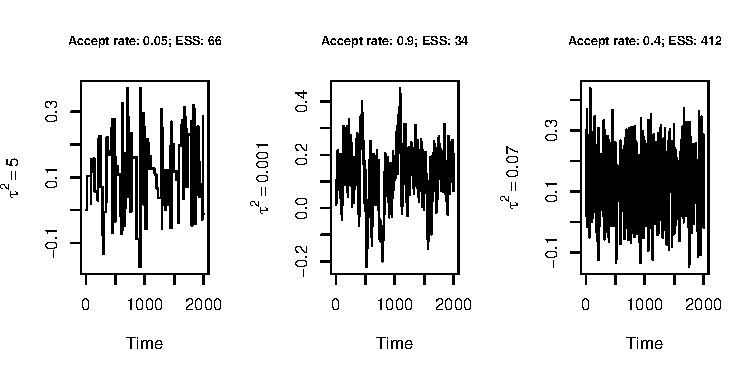
\includegraphics[width=\maxwidth]{figure/gumbel-plots-1} 

\end{knitrout}

\end{frame}


\frame{
\sffamily
\frametitle{The Metropolis-Hastings algorithm}
\begin{itemize}

\item {\bf Example (Nonlinear binomial regression):} We'll consider next a binomial regression for data on the number of adult flour beetles killed after five
hours of exposure to various levels of gaseous carbon disulphide (CS$_{2}$) (from Bliss (1935, Annals of Applied Biology).
$$
P(\mbox{death}\mid w_{i})\equiv h(w_{i})=\left[\frac{\exp(x_{i})}{1+\exp(x_{i})}\right]^{m_{1}}
$$
 where $m_{1}>0$, $w_{i}$ is the known covariate (dose), and $x_{i}=\frac{w_{i}-\mu}{\sigma}$,
where $\mu\in R^{1}$ and $\sigma^{2}>0$.
This problem is more complicated than the previous one in two ways:  Now the unknown paramater vector $\bftheta = (\mu, \sigma, m_{1})$ is three-dimensional, and the last two parameters are restricted to be positive!
\end{itemize}
}


\frame{
\sffamily
\frametitle{The Metropolis-Hastings algorithm}
\begin{itemize}

\item {\bf Example (binomial regression, cont):}  For the positive parameters, we need to use non-negative priors:
\begin{align*}
\mu & \sim N(c_{0},d_{0})   &  \sigma^{2} & \sim IG(e_{0},f_{0})   &   m_{1} & \sim Ga(a_{0},b_{0})
\end{align*}

A Gaussian random walk directly on $\theta$ is not a great idea (you would be automatically rejecting every time you generate negative values for either $\sigma$ or $m_1$).

\vspace{1mm}

\alert{However, a (trivariate!) Gaussian random walk for $(\mu, \log \sigma, \log m_1)$ is feasible and does not lead to automatic rejections. }

\vspace{1mm}

(Another alternative is to use a reflecting Gaussian random walk (this is an option in NIMBLE), but I will not pursue that idea further.)
\end{itemize}
}


\frame{
\sffamily
\frametitle{The Metropolis-Hastings algorithm}
\begin{itemize}

\item {\bf Example (binomial regression, cont):}  Since we work with a transformation of the parameters, there are two ways to derive the algorithm (they lead to different formal expressions, but they are equivalent!):
\begin{enumerate}
\item Do a transformation so that the problem is reformulated as sampling from $p( z_1, z_2, z_3 \mid \bfy)$ where $z_1 = \mu$, $ z_2 = \log \sigma$ and $z_3 = \log m_1$ instead of $p(\mu, \sigma, m_1 \mid \bfy)$.  Once samples $z_1^{(1)}, \ldots, z_1^{(B)}$ and $z_2^{(1)}, \ldots, z_2^{(B)}$ and $z_3^{(1)}, \ldots, z_3^{(B)}$ have been generated, samples $\sigma^{(1)}, \ldots, \sigma^{(B)}$ and $m_1^{(1)}, \ldots, m_1^{(B)}$ can be constructed by letting $\sigma^{(b)} = \exp\{ z_2^{(b)} \}$ and $m_1^{(b)} = \exp\{ z_3^{(b)} \}$
 
\item Keep the original target $p(\mu, \sigma, m_1 \mid \bfy)$ but think of your proposal as being a trivariate combination of a Gaussian and log-Gaussian distribution rather than a Gaussian (and recognize that your proposal is almost symmetric, but not quite!).
\end{enumerate}

Note that, in both cases, a Jacobian is going to be involved.
\end{itemize}
}



\frame{
\sffamily
\frametitle{The Metropolis-Hastings algorithm}
\begin{itemize}

\item {\bf Example (binomial regression, cont):}  Taking the second route, the proposal distribution is
{\small \begin{multline*}
p( \vartheta_1, \vartheta_2, \vartheta_3 \mid \mu, \sigma, m_1) = \frac{1}{(2\pi)^{3/2}} \frac{1}{\vartheta_2 \vartheta_3} \left| \bfOmega \right|^{-1/2}  \\
%
\exp\left\{ -\frac{1}{2} 
\left( \begin{matrix} 
\vartheta_1 - \mu \\
\log \vartheta_2 - \log \sigma \\
\log \vartheta_3 - \log m_1 
\end{matrix}\right)^T
\bfOmega^{-1}
\left( \begin{matrix} 
\vartheta_1 - \mu \\
\log \vartheta_2 - \log \sigma \\
\log \vartheta_3 - \log m_1 
\end{matrix}\right)
\right\}
\end{multline*}
}

Note that $\bfOmega$ does not have to be diagonal, so the moves could (and, turns out, should!) be correlated.  The acceptance probability is
{\scriptsize
$$
\rho(\vartheta_1, \vartheta_2, \vartheta_3, \mu, \sigma, m_1) = 
\min \left\{ 1,
\frac{ p(\bfy|\vartheta_1, \vartheta_2, \vartheta_3)p(\vartheta_1,\vartheta_2, \vartheta_3)}
{p(\bfy|\mu, \sigma, m_1)p(\mu, \sigma, m_1)}
%
\alert{\frac{\vartheta_2 \vartheta_3}{\sigma m_1}} \right\}
$$
}
\end{itemize}
}





\frame{
\sffamily
\frametitle{The Metropolis-Hastings algorithm}

\begin{itemize}

\item {\bf Example (binomial regression, cont):} In the file \texttt{mh-bliss.R} we implement the first of these two approaches (because that allows us to use NIMBLE's provided MCMC algorithms).
\begin{enumerate}
\item To tune the proposal variance, we  run the algorithm once with a diagonal proposal variance/covariance matrix  for the three parameters.
\item We then rerun with the proposal covariance matrix for the trivariate Gaussian proposal equal to   $ = \frac{2.38^2}{d} \Var\left\{ (\mu, \log\sigma, \log m_1)^T \mid \bfy \right\}$.  (In this case $d=3$.)
\end{enumerate}

We'll revisit this when we talk about adaptive Metropolis-Hastings in which we learn the right proposal covariance.

\end{itemize}
 
}



\frame{
\sffamily
\frametitle{The Metropolis-Hastings algorithm}
\begin{itemize}
\item The magic numbers $\frac{2.38^2}{d} \Var(\bftheta | \bfy)$ for proposals and $44 \%$ acceptance rates for unidimensional problems and $23 \%$ for multivariate problems comes from \cite{gelman1996efficient} \cite{roberts1997weak} and \cite{roberts2001optimal}, which derived general theoretical results and  performed experiments on a Gaussian.

\item Since, with enough data, most posteriors are approximately Gaussian, these are reasonable rules of thumb!

\item Note that, because we are making two independent runs, the fact that we change the variance of the chain is not (conceptually) an issue as it does not invalidate the Markov property.

\item If a good approximation for $\Var(\bftheta | \bfy)$ is available (rarely the case) then the preliminary run can be skipped.
\end{itemize}
}



\frame{
\sffamily
\frametitle{The Metropolis-Hastings algorithm}

In the independent Metropolis-Hastings, given $\theta^{(t)}$:
\begin{enumerate}
\item Generate $\vartheta^{(t+1)} \sim g\left( \vartheta \right)$.
\item Take 
$$
\theta^{(t+1)} = \begin{cases}
\vartheta^{(t+1)} & \mbox{with probability }\,  \rho\left(\vartheta^{(t+1)}, \theta^{(t)}\right) \\
\theta^{(t)}  & \mbox{with probability }\,  1 - \rho\left(\vartheta^{(t+1)}, \theta^{(t)}\right)
\end{cases}  ,
$$
where
$$
 \rho\left(\vartheta^{(t+1)}, \theta^{(t)}\right) = \min\left\{ 
 1,
 %
 \frac{p\left(\vartheta^{(t+1)} \mid \bfy\right) }{p\left(\theta^{(t)} \mid \bfy\right)}
 \frac{g\left(\theta^{(t)} \right)}{g\left(\vartheta^{(t+1)} \right)}
 \right\} .
$$

\vspace{1mm}

\alert{You have to be careful to choose an instrumental distribution $g$ that has heavier tails than the target.}
\end{enumerate}
}



\frame{
\sffamily
\frametitle{The Metropolis-Hastings algorithm}
\begin{itemize}
\item  {\bf Example (autoregressive models):  }  Consider a zero-mean autoregressive process of the form 
\begin{align*}
y_t &= \phi y_{t-1} + \epsilon_t    &    \epsilon_t &\sim \normal(0, \sigma^2)
\end{align*}
where $\sigma^2$ is known and $\phi$ is unknown.  It is customary to assume that the process is stationary, which requires $y_1 \sim \normal\left( 0, \frac{\sigma^2}{1 - \phi^2} \right)$ and a prior for $\phi
$ with support only on $(-1,1)$ (e.g., a uniform).  
\end{itemize}
}



\frame{
\sffamily
\frametitle{The Metropolis-Hastings algorithm}
\begin{itemize}
\item  {\bf Example (autoregressive models, cont):  }  The posterior distribution for this problem is
\begin{multline*}
p(\phi \mid \bfy) \propto \left(1 - \phi^2 \right)^{\frac{1}{2}} 
\exp\left\{ -\frac{(1 - \phi^2)}{\sigma^2} y_1^2 \right\}  \\
%
\exp\left\{ -\frac{1}{2\sigma^2} \left[ \phi^2 \sum_{t=2}^{T} y_{t-1}^2 - 2\phi\sum_{t=2}^{T} y_ty_{t-1} \right]   \right\}  \ind_{(-1 < \phi < 1)}
\end{multline*}

Note that this posterior IS NOT tractable.  However, if you drop the first two terms (which come from $p(y_1 \mid \phi)$) then the remainder looks like the kernel of a Gaussian distribution.
\end{itemize}
}



\frame{
\sffamily
\frametitle{The Metropolis-Hastings algorithm}
\begin{itemize}
\item  {\bf Example (autoregressive models, cont):  }  This suggest using independent proposal for you MCMC of the form
\begin{align*}
\vartheta \sim \normal\left( \vartheta \mid
\frac{\sum_{t=2}^{T} y_t y_{t-1}}{\sum_{t=2}^{T}y_t^2},
\frac{\sigma^2}{\sum_{t=2}^{T}y_t^2}
\right) \ind_{(-1 < \vartheta < 1)}
\end{align*}

Because this distribution contains most of the information in the data, we expect it to be very close to the true posterior.  The acceptance rate in this case is simply
\begin{align*}
\rho(\vartheta, \phi) = \min\left\{ 1,  \sqrt{\frac{1 - \vartheta^2}{1 - \phi^2}} \exp\left\{ \frac{y_1^2(\vartheta^2 - \phi^2)}{2\sigma^2}
 \right\} \right\}
\end{align*}

Which depends only on the term we dropped out when generating our proposal!
\end{itemize}
}





\frame{
\sffamily
\frametitle{The Metropolis-Hastings algorithm}
\begin{itemize}
\item The Metropolis-Hastings algorithm is very general and we have a lot of freedom in choosing proposals.  However, there are some constraints:
\begin{itemize}
\item For the algorithm to work, we need to ensure that the chain is irreducible.  One way to ensure this is ensure that the support of the proposal $q(\vartheta | \theta)$ contains the support of $f$ for every $\theta$.

%% \item We also need to ensure the chain is reversible, which (roughly speaking) requires that if $q(\vartheta \mid \theta) > 0$  then also $q(\theta \mid \vartheta) > 0$

\item Positive recurrence is typically not an issue once you have ensured irreducibility. 

\item Aperiodicity is also typically not a problem (for most situation you would actually need to do some work to get a periodic chain).
\end{itemize}
\end{itemize}
}



\frame{
\sffamily
\frametitle{The Metropolis-Hastings algorithm}
\begin{itemize}
\item Why does the Metropolis-Hastings work?  Because of the reversibility of the chain. This ensures that the stationary distribution is the posterior. 

\item Note that the transition kernel associated with the Metropolis-Hastings algorithm is 
$$
K(\theta_{t-1}, \theta_t) = \rho(\theta_{t}, \theta_{t-1})q(\theta_t, \theta_{t-1}) + \{ 1 - r(\theta_{t-1}) \} \delta_{\theta_{t-1}(\theta_t)}
$$
where $\delta_x$ denotes the Dirac mass at $x$ and 
$$
r(\theta) = \int \rho(\vartheta, \theta) q(\vartheta \mid \theta) \dd \vartheta
$$

\item This kernel satisfies the detailed balance equations.
\end{itemize}
}








\frame{
\sffamily
\frametitle{Diagnostics for MCMC algorithms}
\begin{itemize}
\item  Recall that, although Metropolis-Hastings algorithm work if we run them long enough, the fact that samples are dependent presents challenges:
\begin{itemize}
\item Convergence.
\item Mixing.
\end{itemize}

\item \alert{Mixing:}  As with every Monte Carlo algorithm an important question is how many samples should be generated in order to have estimates of the parameters with a reasonable level of accuracy. 
\begin{itemize}
\item However, because samples are (most usually positively) correlated, standard theory (standard central limit theorems, Chebyshev's inequality, etc.) does not apply here!

\item Mixing is related to how fast the chain explores the posterior distribution.
\end{itemize}
\end{itemize}
}



\frame{
\sffamily
\frametitle{Diagnostics for MCMC algorithms}
\begin{itemize}
\item \alert{Convergence:}  An additional question when using MCMC algorithms that is not a concern in standard Monte Carlo is how many of the initial observations need to be discarded before we can perform any inference.  
\begin{itemize}
\item Remember that, unless your initial state is sampled from the stationary distribution, the samples of your chain are only distributed as the stationary distribution when the number of iterations goes to infinity.

\item In practice, if your posterior is unimodal, you just want your initial state to be close to the high-probability areas.

\item When posterior is multimodal, convergence can be a huge issue.
\end{itemize}
\end{itemize}
}



\frame{
\sffamily
\frametitle{Diagnostics for MCMC algorithms}
\begin{itemize}
\item These two questions are interrelated, but are not identical.  For example, you can accelerate convergence to the posterior by carefully selecting the initial state of your chain even if the chain mixes slowly.  On the other hand, even if your initial state is really distributed from the stationary distribution (e.g., by using perfect sampling), you might need to run a very long chain to have an acceptable level of uncertainty in your estimates if the autocorrelation in the parameters of interest is very high.

\item Time series plots of the realized chains (the so-called \textit{trace} plots) provide visual intuition about these two concepts, and can be used as an informal check (which should be supplemented with some of the formal techniques discussed later).
\end{itemize}
}






\frame{
\sffamily
\frametitle{Diagnostics for MCMC algorithms}
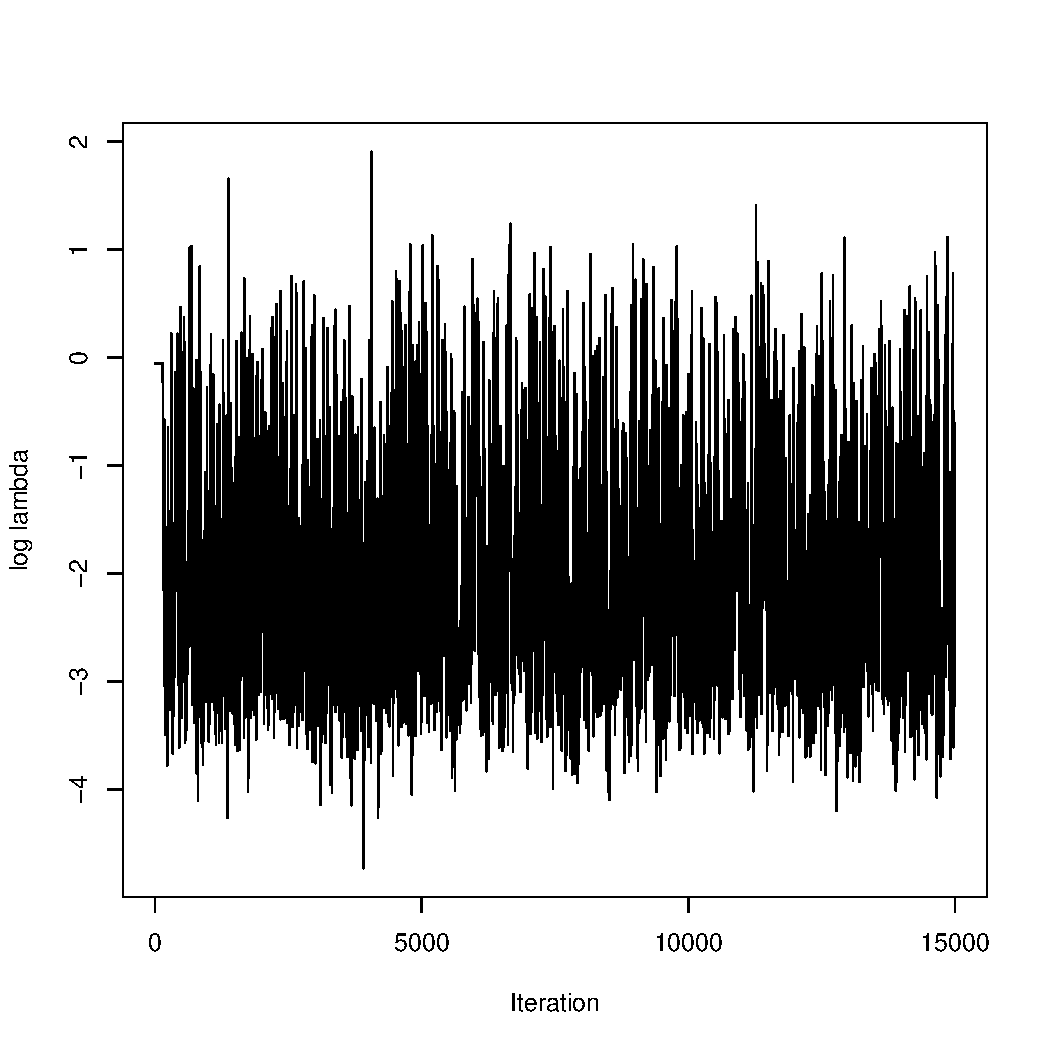
\includegraphics[height=5.4cm,angle=0]{plots/mod_aucor_good_initial.pdf}
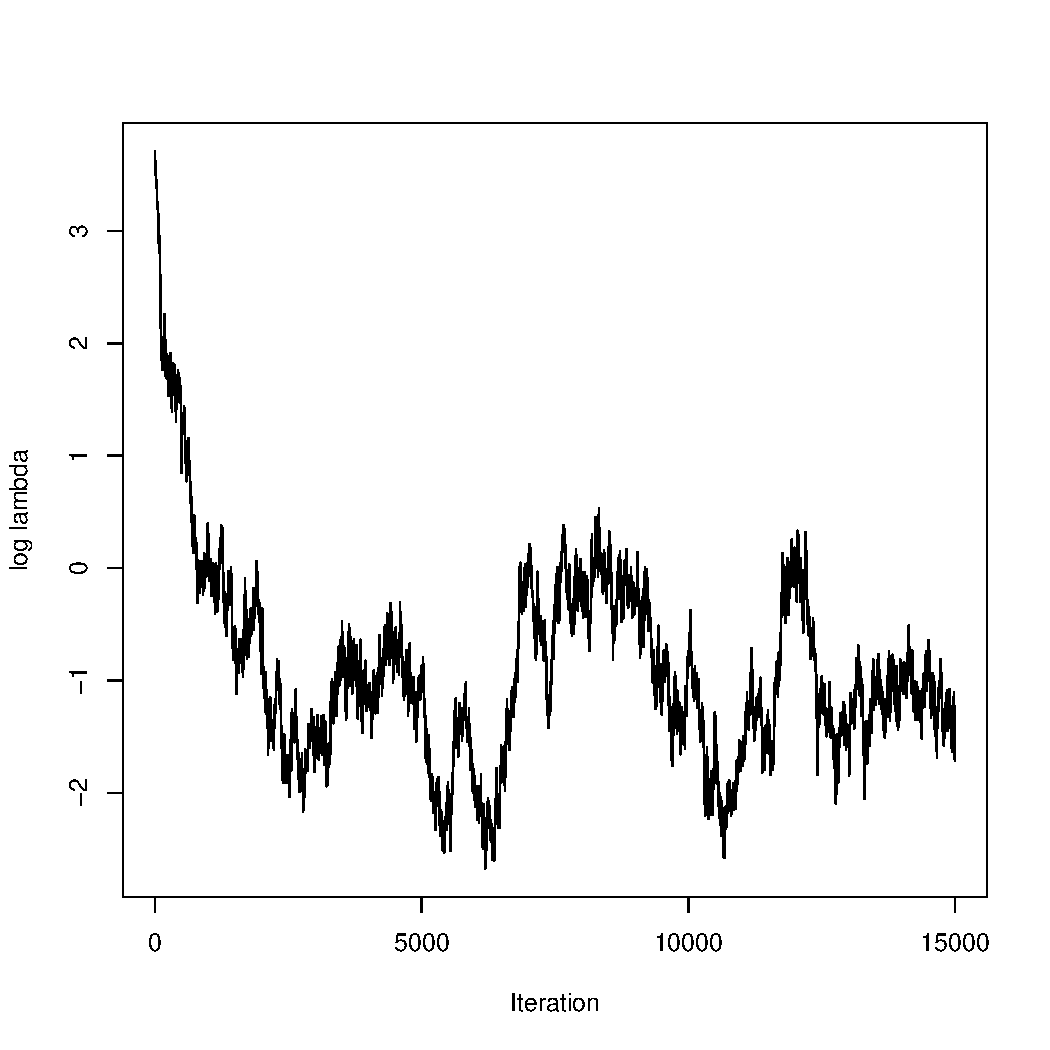
\includegraphics[height=5.4cm,angle=0]{plots/high_aucor_bad_initial.pdf}
}




\frame{
\sffamily
\frametitle{Checking for convergence}
\begin{itemize}
\item Generally speaking, determining \textit{a priori} how many iterations are needed for burn-in in not possible.  Indeed, except for some special cases, general theory about the behavior of the algorithm (e.g., the value of the second largest eigenvalue of the kernel function) is not easy to derive.

\item For this reason, most practical algorithms to monitor convergence look at the time-series behavior of a small number of selected parameters (or functions of parameters).
\begin{itemize}
\item Selecting which parameters need to be monitored is tricky and model dependent.  In high-dimensional models I usually monitor either the likelihood or the posterior, a small (random) subset of the main first-stage parameters, and a couple of important hyperparameters.

\item All criteria here are implemented in the \texttt{R} package \texttt{CODA}.
\end{itemize}

\item We typically cannot ensure convergence, just argue that there is no evidence of \text{lack of convergence}.

\end{itemize}
}





\frame{
\sffamily
\frametitle{Checking for convergence (Multi-chain methods)}
\begin{itemize}
\item As the name suggests multi-chain methods use $M > 1$ realizations of the algorithm (each of length $B$, typically started from ``over dispersed'' values) and compare the output of the chains.  Once the statistical properties of the realizations appear to be similar, the chains are deemed to have converged.

\item One example of this type of approach was introduced by \cite{GeRu92} who propose to monitor a statistic that compares the average within-chain variability against the between-chain variability:
$$
R = \left( \frac{B-1}{B} + \frac{M+1}{M} \frac{Z_B}{W_B} \right) \frac{\nu_B}{\nu_B - 2} ,
$$
where $Z_B$ is an estimate of between-chain variability, $W_B$ is an estimate of within-chain variability and $\nu_B$ is the approximate number of degrees of freedom. 
\end{itemize}
}




\frame{
\sffamily
\frametitle{Checking for convergence (Multi-chain methods)}
If $\xi = h(\theta)$ is the quantity of interest being monitored, define
\begin{align*}
\bar{\xi}_m &= \frac{1}{B} \sum_{b=1}^{B} \xi_m^{(b)}   &  \bar{\xi} &= \frac{1}{M} \sum_{m=1}^{M} \bar{\xi}_m & s_m^2 &= \frac{1}{B} \sum_{b=1}^{B} \left(\xi_m^{(b)} - \bar{\xi}\right)^2 
\end{align*}

Then
\begin{align*}
Z_B &= \frac{1}{M} \sum_{m=1}^{M} \left(\bar{\xi}_m - \bar{\xi}\right)^2   &  W_B &= \frac{1}{M} \sum_{m=1}^{M} s_m^2  
\end{align*}
and
$$
 \nu_B = \frac{2\left( \frac{B-1}{B}W_B + \frac{M+1}{M} Z_B \right)^2}{W_B}
$$

}






\frame{
\sffamily
\frametitle{Checking for convergence (Multi-chain methods)}
\begin{itemize}
\item We have $B Z_B/W_B \sim F_{M-1, 2W_B^2/\varpi_B}$ approximately, where
$$
\varpi_B =  \frac{1}{M^2} \left[ \sum_{m=1}^{M} s_m^4 - \frac{1}{M} \left( \sum_{m=1}^{M} s_m^2 \right)^2 \right]
$$

\item Once the chains have converged we expect $R \to 1$, so the approximate distribution can be used to test convergence at different values of $B$.

\item Samples from different chains are then combined together for computing any expectation of interest.
\end{itemize}
}




\begin{frame}[fragile]
\sffamily
\frametitle{Checking for convergence (Multi-chain methods)}


\begin{center}
\hspace{-0.9cm}
\begin{tabular}{lr}
\begin{minipage}{5.5cm}





\begin{knitrout}\tiny
\definecolor{shadecolor}{rgb}{0.969, 0.969, 0.969}\color{fgcolor}\begin{kframe}
\begin{alltt}
\hlkwd{library}\hlstd{(coda,} \hlkwc{warn.conflicts} \hlstd{=} \hlnum{FALSE}\hlstd{)}

\hlstd{chains} \hlkwb{<-} \hlkwd{as.mcmc.list}\hlstd{(}
    \hlkwd{list}\hlstd{(}\hlkwd{as.mcmc}\hlstd{(smp1),} \hlkwd{as.mcmc}\hlstd{(smp2)))}
\hlstd{gr} \hlkwb{=} \hlkwd{gelman.diag}\hlstd{(chains,} \hlkwc{autoburnin} \hlstd{=} \hlnum{FALSE}\hlstd{)}
\hlkwd{print}\hlstd{(gr)}
\end{alltt}
\begin{verbatim}
## Potential scale reduction factors:
## 
##          Point est. Upper C.I.
## logm1        263.30     1314.9
## logsigma       4.74       10.3
## mu             7.15       15.9
## 
## Multivariate psrf
## 
## 259
\end{verbatim}
\end{kframe}
\end{knitrout}

\end{minipage}
%&
\begin{minipage}{5.5cm}
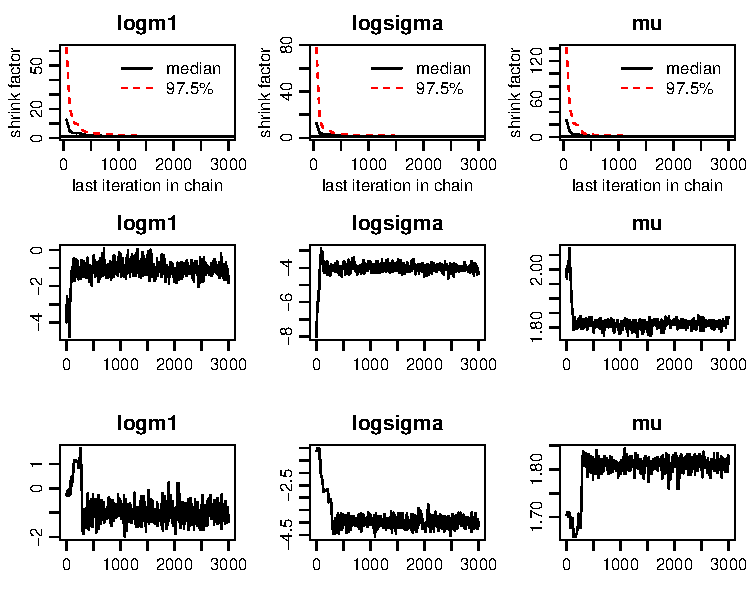
\includegraphics[width=5.4cm,angle=0]{plots/bliss-gelman-rubin.pdf}
\end{minipage}
\end{tabular}
\end{center}
\end{frame}




\frame{
\sffamily
\frametitle{Checking for convergence (Multi-chain methods)}
\begin{itemize}
\item I tend to prefer multi-chain methods.  One advantage is that they can be naively parallelized.

\item However, finding over-dispersed initial points can be hard.  For example, if the posterior is multimodal and you do not start the chain at least once on each mode you might never find out.

\item For slow-mixing chains, inferences based on a single long chain might be more accurate than the inferences based on many small chains put together.  (However, this is an issue mostly if computational resources are limited.)
\end{itemize}
}





\frame{
\sffamily
\frametitle{Checking for convergence (Single-chain methods)}
\begin{itemize}
\item An alternative to multi-chain methods is to use a single long chain and see if the properties of the chain have ``stabilized''.

\item More specifically, we can divide the original chain of length $B$ into $M$ sections of approximately equal length and compare their spectral densities.

\item In particular \cite{Ge92} proposes to compare the first and second half of the chain (i.e., use $M=2$).  The algorithm is implemented in the \texttt{R} function \texttt{geweke.diag} and \texttt{geweke.plot}.
\item Interestingly, the most recent edition of Gelman et al. Bayesian Data Analysis suggests to use the Gelman-Rubin approach with each chain split into two to assess both mixing and convergence.
\end{itemize}
}




\frame{
\sffamily
\frametitle{Mixing}
\begin{itemize}
\item Again, it must be emphasized that mixing is a subtly different problem from convergence.

\item Note that a chain that mixes slowly, if started on a low-probability region of the space, might take a long time to converge.  However, if we start it in a high probability region convergence is much less of an issue.

\item A simple way to decide how long the algorithm must be run \textit{after} the burn-in period is to evaluate the variance of the estimators.
\end{itemize}
}





\frame{
\sffamily
\frametitle{Mixing}
\begin{itemize}
\item Let $h$ be an integrable function.  Recall that we aim at approximating $\E_{\bftheta \mid \bfy}\left\{ h(\bftheta) \right\} \approx \frac{1}{B} \sum_{b=1}^{B} h\left(\bftheta^{(b)}\right)$

\vspace{1mm}

\item If the samples $\bftheta^{(1)}, \ldots, \bftheta^{(B)}$ were independent, the variance of the estimator would be equal to $\frac{\Var \left\{ h(\bftheta) \right\} }{B}$.  In practice a rough estimate of $\Var \left\{ h(\bftheta) \right\}$ can also be obtained by Monte Carlo.

\vspace{1mm}

\item From Markov chain theory, it is easy to show that for an MCMC that has converged the variance of the same estimator is $\tau_h \frac{\Var h(\bftheta)}{ B}$ where $\tau_h$ is the integrated autocorrelation: $\tau_h = 1 + 2 \sum_{t=1}^{\infty} \rho_t $, with $\rho_t$  the autocorrelation at lag $t$.

\item We call $\frac{B}{\tau_h}$ the equivalent sample size.
\end{itemize}
%so we call $\frac{n}{\tau_g}$ the effective sample size.  Issues:  highly dependent on $g$, it does not take into account the execution time of each step.
% For any $g$ it is possible to show that $\tau_g \ge \frac{1- \lambda_2}{1 + \lambda_2}$, where $\lambda_2 is the second largest eigenvalue
}






\frame{
\sffamily
\frametitle{Mixing}
\begin{itemize}
\item The equivalent sample size calculation is implemented in \texttt{CODA} through the function \texttt{effectiveSize}.

\item Note that the equivalent sample size will be different for different parameters.  That means that a given number of iterations might be enough for one parameter, but not for another.

\item Some people like to ``thin" their chain (retain every X number of iterations and drop the rest) as a way to decrease $\tau_h$.  However, this also reduces $B$!  
\begin{itemize}
\item \citet{maceachern1994subsampling} proved the tradeoff is not favorable.
\item Unless storage (in memory or on disk) is an issue, thinning is not a good idea.
\end{itemize}
\end{itemize}
}










\frame{
\sffamily
\frametitle{Beyond the Metropolis-Hasting algorithm}
\begin{itemize}
\item  Our description of the Metropolis-Hastings algorithm involved a single joint proposal for all entries of $\bftheta$.

\item However, even using adaptive algorithms as the ones described later, making good proposals in high dimensions is difficult.  It would be helpful if we could work with one dimension (or a small number of dimensions) at a time and make low-dimensional updates.

\item Such approach actually works, and can be justified by considering mixtures of kernels!
\end{itemize}
}






\frame{
\sffamily
\frametitle{Mixtures of kernels}
\begin{itemize}
%\item You do not have to update parameters one at a time, you might decide to update groups of parameters simultaneously $\Rightarrow$  \alert{Blocking} (usually improves the convergence).

%\item Indeed, updating parameters individually usually works best when parameters are (approximately) orthogonal (independent) a posteriori.  When they are highly correlated a posteriori, it is preferable to sample them jointly using proposals that acknowledge that correlation!

\item You do not have to update parameters one at a time, you might decide to update subgroups of parameters.

\vspace{2mm}

\item In addition to random sweeps, you can run through the kernels sequentially.  Justification is based on a composition of kernels rather than a mixture.  

\vspace{2mm}

\item In sequential sweeps not all kernels need to be used with the same frequency (just like kernels do not have to be chosen with the same probability when doing random sweeps).

\vspace{2mm}

\item  It is important that all variables are updated at least once (but they could be updated multiple times).
\end{itemize}
}







\frame{
\sffamily
\frametitle{The Gibbs sampler as a special case of the Metropolis}
\begin{itemize}
\item  We can take our argument one step further.  Suppose that you are working with the component-wise (or block-wise!) MH algorithm and that you are able to directly sample from the full conditional, so that you decide to use independent proposal (rather than a random-walk proposals) with
$$
q(\vartheta_i \mid \theta_i) = p(\vartheta_i \mid \theta_1, \ldots, \theta_{i-1}, \theta_{i+1}, \ldots, \theta_{p}).
$$

\item Note that in that case the acceptance probability is $1$ for all samples (the Hastings ratio is the reciprocal of the ratio of posteriors), and your MH algorithm reduces to (sequentially) sampling from all full conditional distributions!
\begin{itemize}
\item This is what we called the Gibbs sampler.
\end{itemize}


\end{itemize}
}

\begin{frame}[fragile] 
\sffamily
\frametitle{The Gibbs sampler as a special case of the Metropolis}
{\small
\begin{itemize}
\item {\bf Example (litters GLMM):} NIMBLE's default samplers use a Gibbs-based strategy of cycling through individual parameters with either Metropolis or conjugate samplers assigned individually:



\begin{knitrout}\tiny
\definecolor{shadecolor}{rgb}{0.969, 0.969, 0.969}\color{fgcolor}\begin{kframe}
\begin{alltt}
\hlstd{thin} \hlkwb{<-} \hlnum{10}
\hlcom{# thinning _only_ to reduce time of plotting }
\hlstd{conf} \hlkwb{<-} \hlkwd{configureMCMC}\hlstd{(glmmModel,} \hlkwc{thin} \hlstd{= thin)}
\hlstd{conf}\hlopt{$}\hlkwd{getSamplers}\hlstd{(}\hlkwd{c}\hlstd{(}\hlstr{'a'}\hlstd{,}\hlstr{'b'}\hlstd{,}\hlstr{'p[1,1]'}\hlstd{,}\hlstr{'p[2,1]'}\hlstd{))}
\end{alltt}
\begin{verbatim}
## [[1]]
## RW sampler: a[1]
## [[2]]
## RW sampler: a[2]
## [[3]]
## RW sampler: b[1]
## [[4]]
## RW sampler: b[2]
## [[5]]
## conjugate_dbeta_dbin sampler: p[1, 1]
## [[6]]
## conjugate_dbeta_dbin sampler: p[2, 1]
\end{verbatim}
\end{kframe}
\end{knitrout}
While Gibbs sampling is often effective, when there is strong posterior dependence, it can have bad convergence and bad mixing.
\end{itemize}

}
\end{frame}

\frame{
\sffamily
\frametitle{The Gibbs sampler as a special case of the Metropolis}

\begin{itemize}
\item {\bf Example (litters GLMM):} Here are traceplots (see \texttt{gibbs-litters.R} for the code).
\begin{center}
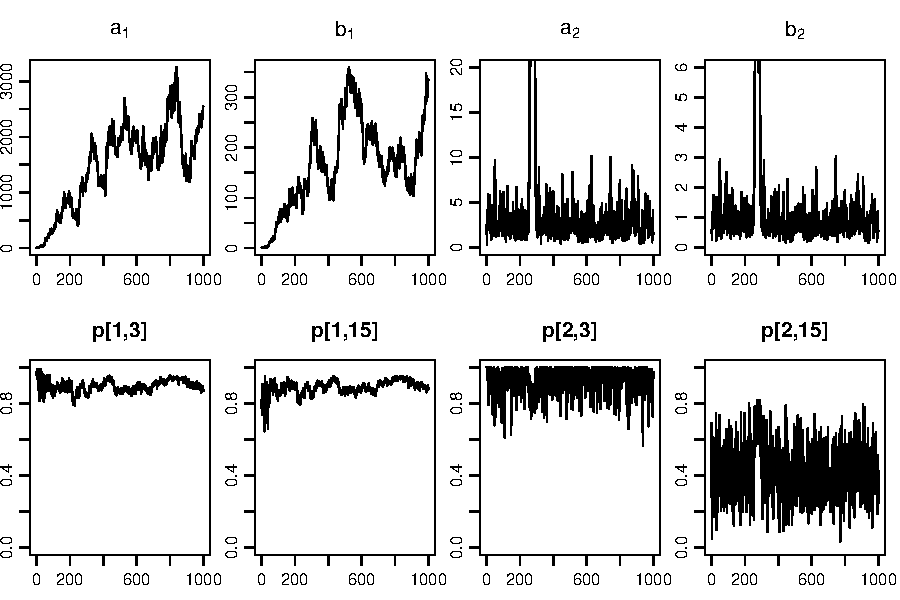
\includegraphics[width=2.8in]{plots/gibbs-litters.pdf}
\end{center}

Despite knowing the exact conditional distributions for $p$, the poor mixing of the hyperparameters in the priors for $p$ produce bad mixing for $p$ values for the first group.
\end{itemize}
}



\frame{
\sffamily
\frametitle{General design rules for MH algorithms}
\begin{itemize}
\item  MH algorithms are highly modular but there is a trade-off between simplicity of implementation, speed, and mixing.

\item Block highly-correlated parameters (but when there is not strong dependence individual samplers can move further than a blocked Gaussian).

\item Reparameterizing the model to center it or to make parameters less correlated is usually helpful!  This is easy to do in the context of linear model, but not always so in other case (computing information matrices might provide hints).

\item As a rule of thumb, you want to ``integrate out'' as many parameters as you can before attempting to use any Metropolis/Gibbs steps.
However, introducing latent variables can greatly simplify algorithms and in some cases improve mixing.
\end{itemize}
}






\frame{
\sffamily
\frametitle{Blocking}

{\footnotesize
\begin{itemize}
\item {\bf Example (litters GLMM):} We saw that univariate sampling worked poorly on the litters GLMM model. This is common in GLMMs -- the dependence between hyperparameters and random effects can impede mixing.

Some strategies for random effects models:

\begin{itemize}
\item analytically integrate over random effects to reduce model dimensionality (not always feasible though feasible here)
\item approximately integrate over random effects (e.g., INLA)
\item expand the blocking to include the random effects
\end{itemize}

In the litters model, we could integrate the $p$'s out of the model and do block sampling on the hyperparameters.

Alternatively, NIMBLE provides a \emph{cross-level} sampler that blocks hyperparameters with random effects when the random effects have a conjugate structure. This blocking is equivalent to marginalizing the $p$'s. This works much better than Metropolis-based blocking because the dependence is nonlinear.

\end{itemize}
}
}


\begin{frame}[fragile]
\sffamily
\frametitle{Blocking}

\begin{itemize}
\item {\bf Example (litters GLMM):}

See \texttt{blocked-litters.R} for NIMBLE code for the blocked sampler.





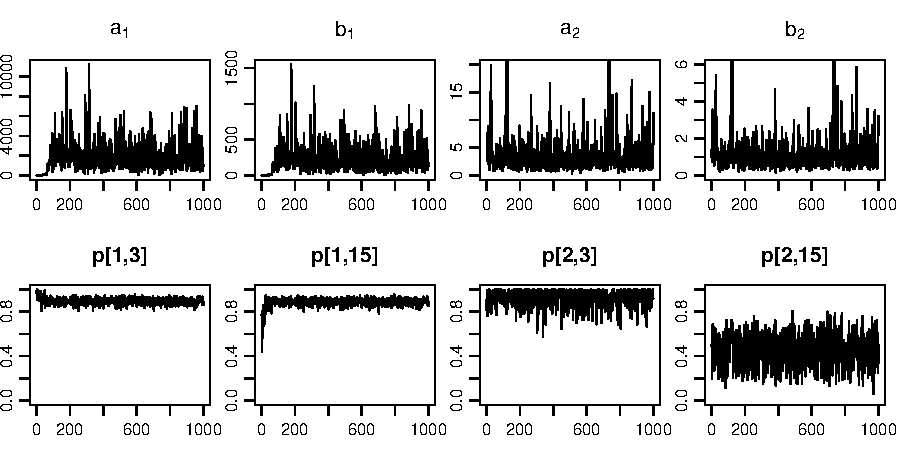
\includegraphics[width=3in]{plots/blocked-litters.pdf}
\end{itemize}
\end{frame}

\frame{
\sffamily
\frametitle{Centering}
\begin{itemize}
\item To illustrate the role of centering, consider a simple linear mixed model (random-intercept model).
\begin{align*}
y_{i,j} \mid \mu, \theta_i & \sim \normal(\eta + \theta_i, \sigma^2) ,  &   \eta &\sim \normal(0, \kappa^2 = \infty)  ,  &  \theta_i & \sim \normal(0, \tau^2) ,
\end{align*}
for $i=1, \ldots, I$ and $j=1, \ldots, J$.

\item The full conditional distributions are
\begin{align*}
\theta_i \mid \eta &\sim \normal \left(  
\frac{ \sum_{j=1}^{J} (y_{i,j} - \eta)/\sigma^2 }{\left( \frac{J}{\sigma^2} + \frac{1}{\tau^2} \right)}, 
\left( \frac{J}{\sigma^2} + \frac{1}{\tau^2} \right)^{-1} 
\right)  ,  \\
%
\eta \mid \theta_1, \ldots, \theta_I &\sim \normal \left(  
\frac{ \sum_{i=1}^{I}\sum_{j=1}^{J} (y_{i,j} - \theta_i)/\sigma^2 }{\left( \frac{IJ}{\sigma^2} + \frac{1}{\kappa^2} \right)}, 
\left( \frac{IJ}{\sigma^2} + \frac{1}{\kappa^2} \right)^{-1} 
\right)  .
\end{align*}
\end{itemize}
}




\frame{
\sffamily
\frametitle{Centering}
\begin{center}
\hspace{-0.8cm}
\begin{tabular}{lr}
\begin{minipage}{5cm}
\vspace{0.2cm}
\begin{itemize}
\item We simulated data with $\eta = 0.8$, $\sigma^2 = 1$ and $\tau^2 = 2$, and ran the algorithm.
\item $\theta_1$ and $\eta$ show high (negative) autocorrelation and slow mixing.
\end{itemize}
\end{minipage}
%&
\begin{minipage}{6cm}
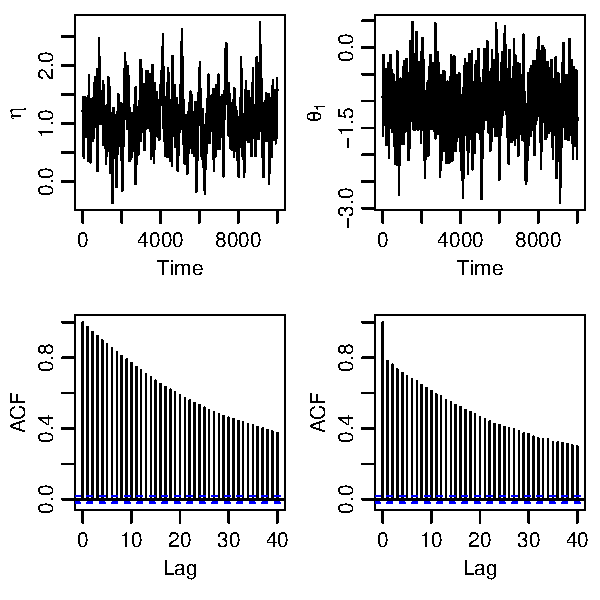
\includegraphics[height=5.7cm,angle=0]{plots/centering1.pdf}
\end{minipage}
\end{tabular}
\end{center}
}




\frame{
\sffamily
\frametitle{Centering}
\begin{itemize}
\item Instead, consider reparameterizing the model so that $\theta^{*}_i = \mu + \theta_i$ so that
\begin{align*}
y_{i,j} \mid \mu, \theta^{*}_i & \sim \normal(\theta^{*}_i, \sigma^2)  ,  &  \theta^{*}_i & \sim \normal(\eta, \tau^2) ,  &   \eta &\sim \normal(0, \kappa^2) .
\end{align*}

\item The full conditional distributions are
\begin{align*}
\theta^{*}_i \mid \eta &\sim \normal \left(  
\frac{ \frac{\sum_{j=1}^{J} y_{i,j}}{\sigma^2} + \frac{\eta}{\tau^2}}{\left( \frac{J}{\sigma^2} + \frac{1}{\tau^2} \right)}, 
\left( \frac{J}{\sigma^2} + \frac{1}{\tau^2} \right)^{-1} 
\right)  ,  \\
%
\eta \mid \theta^{*}_1, \ldots, \theta^{*}_I &\sim \normal \left(  
\frac{ \frac{\sum_{i=1}^{I} \theta^{*}_i}{\tau^2} }{\left( \frac{I}{\tau^2} + \frac{1}{\kappa^2} \right)}, 
\left( \frac{I}{\tau^2} + \frac{1}{\kappa^2} \right)^{-1} 
\right)  .
\end{align*}
\end{itemize}
}





\frame{
\sffamily
\frametitle{Centering}
\begin{center}
\hspace{-0.8cm}
\begin{tabular}{lr}
\begin{minipage}{5cm}
\vspace{0.2cm}
\begin{itemize}
\item We ran this MCMC for the same dataset as before and backtransformed the samples to get $\theta_i = \theta^{*}_i - \eta$.
\item Mixing for $\theta_1$ and $\eta$ is quite good now.
\item See NIMBLE code in \texttt{mh-centering.R}.
\end{itemize}
\end{minipage}
%&
\begin{minipage}{6cm}
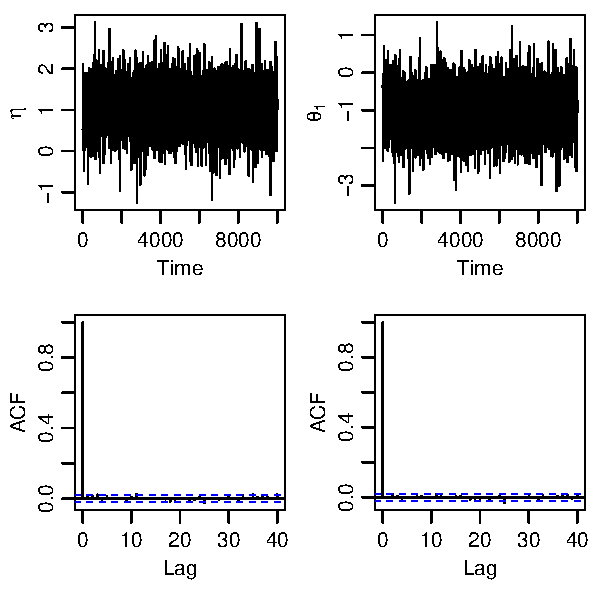
\includegraphics[height=5.7cm,angle=0]{plots/centering2.pdf}
\end{minipage}
\end{tabular}
\alert{Centering is not universally better, but it usually is!}
See \citep{yu2011center} for how to combine centered and uncentered.

\end{center}
}








\frame{
\sffamily
\frametitle{Auxiliary variables}
\begin{itemize}
\item In spite of all the caveats mentioned so far, Gibbs steps are very often preferable because they are simpler to implement.

\item Particularly in high-dimensional problems, making joint proposals is difficult, while univariate random-walk MH steps end up being very inefficient.

\item In many cases computation can be simplified by adding auxiliary variables (we are not interested in them, but they are added for convenience!)

\item This is sometimes called demarginalization:  We look for a model such that, when we marginalize over the auxiliary variables, we recover the original one.

\item This goes against our design criteria, but can dramatically simplify implementation with a moderate cost in terms of mixing.  In some cases, it can even improve mixing!
\end{itemize}
}





\frame{
\sffamily
\frametitle{Auxiliary variables}
\begin{itemize}
\item {\bf Example (Gaussian mixture models):  }  Assume that data is generated from a two-component mixture
$$
y_i \mid \omega, \theta_1, \sigma_1^2, \theta_2, \sigma_2^2 \sim \omega \normal(y_i \mid \theta_1, \sigma_1^2) + (1-\omega) \normal(y_i \mid \theta_2, \sigma_2^2)
$$
for $i=1,\ldots, n$ with priors
\begin{align*}
\omega &\sim \bet(1,1) ,   &   \theta_i &\sim \normal(\mu,\tau^2) ,   &   \sigma^2_i &\sim \IGam(a, c).
\end{align*}

Sampling directly from this model is complicated.  You could try a five-dimensional Gaussian random walk on $(\mbox{logit} \, \omega, \theta_1, \log \sigma_1^2, \theta_2, \log \sigma_2^2)$, but it would be hard to tune.  More importantly, such scheme would not scale very well to mixtures with more components.

\end{itemize}
}



\frame{
\sffamily
\frametitle{Auxiliary variables}
\begin{itemize}
\item {\bf Example (Gaussian mixture models, cont):  }  Augment the model with indicator variables $\xi_1, \ldots, \xi_n$ such that $\xi_i \in \{ 1, 2 \}$ and
$$
y_i \mid \xi_i, \theta_1, \sigma_1^2, \theta_2, \sigma_2^2 \sim \normal(y_i \mid \theta_{\xi_i}, \sigma_{\xi_i}^2) ,
$$
where the $\xi_i$s are iid with 
$$
\Pr(\xi_i = 1 \mid \omega) = \omega = 1 - \Pr(\xi_i = 2 \mid \omega) .
$$
It is clear that if we integrate $\xi_i$ out of the model we recover our original formulation.
\end{itemize}
}




\frame{
\sffamily
\frametitle{Auxiliary variables}
\begin{itemize}
\item {\bf Example (Gaussian mixture models, cont):  }  In the augmented model, the posterior distribution is proportional to
\begin{multline*}
\left\{ \prod_{i=1}^{n} \normal \left(y_i \mid \theta_{\xi_i}, \sigma_{\xi_i}^2 \right) \right\} 
\left\{ \prod_{i=1}^{n} \omega^{\sum_{i=1}^{n} \ind_{\{ \xi_i = 1 \}}} \left( 1 - \omega\right)^{\sum_{i=1}^{n} \ind_{\{ \xi_i = 2 \}}}  \right\} \\
%
 \bet(\omega \mid 1, 1) \left\{ \prod_{i=1}^{2} \normal(\theta_i \mid \mu, \tau^2) \right\}  \left\{ \prod_{i=1}^{2} \IGam(\sigma^2_i \mid a, c) \right\}
\end{multline*}


\end{itemize}
}



\frame{
\sffamily
\frametitle{Auxiliary variables}
\begin{itemize}
\item {\bf Example (Gaussian mixture models, cont):  }  The full conditionals reduce to:
\begin{enumerate}
\item $\Pr\left( \xi_i = 1 \mid \cdots \right) = \frac{\omega \frac{1}{\sigma_1}\exp\left\{ -\frac{(y_i - \theta_1)^2}{2\sigma^2_1}  \right\}}{\omega\frac{1}{\sigma_1}\exp\left\{ -\frac{(y_i - \theta_1)^2}{2\sigma^2_1}  \right\} + (1-\omega)\frac{1}{\sigma_2}\exp\left\{ -\frac{(y_i - \theta_2)^2}{2\sigma^2_2}  \right\}}$, while $\Pr\left( \xi_i = 2 \mid \cdots \right) = 1 - \Pr\left( \xi_i = 1 \mid \cdots \right)$.

\vspace{1.5mm}

\item $\omega \mid \cdots \sim \bet\left( 1 + n_1,  1 + n_2 \right)$ where $m_k = \sum_{i=1}^{n} \ind_{\{ \xi_i = k \}}$.

\vspace{1.5mm}

\item $\theta_k \mid \cdots \sim \normal\left( \frac{\frac{s_k}{\sigma_k^2} + \frac{\mu}{\tau^2}}{\frac{m_k}{\sigma_k^2} + \frac{1}{\tau^2}}, \frac{1}{\frac{m_k}{\sigma_k^2} + \frac{1}{\tau^2}} \right)$ where $m_k = \sum_{i=1}^{n} \ind_{\{ \xi_i = k \}}$ as before and $s_k = \sum_{\{ i : \xi_i = k \}} y_{i}$.

\vspace{1.5mm}

\item $\sigma^2_k \mid \cdots \sim \IGam\left( a + \frac{m_k}{2} , c + \frac{1}{2} \sum_{\{ i : \xi_i =k \}} \{ y_i - \theta_k \}^2 \right)$.

\vspace{1.5mm}

Note that the $\xi_i$s have a nice interpretation, particularly if you are using the mixture model for clustering!
\end{enumerate}
\end{itemize}
}

\begin{frame}[fragile]
\sffamily
\frametitle{Auxiliary variables}

\begin{itemize}
\item {\bf Example (Gaussian mixture models, cont):} Here is the NIMBLE code for such an augmented mixture model.

\begin{knitrout}\scriptsize
\definecolor{shadecolor}{rgb}{0.969, 0.969, 0.969}\color{fgcolor}\begin{kframe}
\begin{alltt}
\hlstd{mixCode} \hlkwb{<-} \hlkwd{nimbleCode}\hlstd{(\{}
    \hlkwa{for}\hlstd{(i} \hlkwa{in} \hlnum{1}\hlopt{:}\hlstd{n) \{}
        \hlstd{y[i]} \hlopt{~} \hlkwd{dnorm}\hlstd{(theta[ksi[i]}\hlopt{+}\hlnum{1}\hlstd{],} \hlkwc{var} \hlstd{= sigma2[ksi[i]}\hlopt{+}\hlnum{1}\hlstd{])}
        \hlstd{ksi[i]} \hlopt{~} \hlkwd{dbern}\hlstd{(omega)}
    \hlstd{\}}
    \hlstd{omega} \hlopt{~} \hlkwd{dbeta}\hlstd{(}\hlnum{1}\hlstd{,} \hlnum{1}\hlstd{)}
    \hlkwa{for}\hlstd{(j} \hlkwa{in} \hlnum{1}\hlopt{:}\hlnum{2}\hlstd{) \{}
        \hlstd{theta[j]} \hlopt{~} \hlkwd{dnorm}\hlstd{(mu, tau2)}
        \hlstd{sigma2[j]} \hlopt{~} \hlkwd{dinvgamma}\hlstd{(a, c)}
    \hlstd{\}}
\hlstd{\})}
\end{alltt}
\end{kframe}
\end{knitrout}
\end{itemize}
\end{frame}

\frame{
\sffamily
\frametitle{Auxiliary variables}

\begin{itemize}
\item {\bf Example (Gaussian mixture models, cont):} The code in \texttt{mixture-faithful.R} shows both the original and augmented versions of the two-component mixture model for R's Old Faithful dataset. For the original version, we need a user-defined mixture density.

Here's the posterior inference for the mixture weights and membership.

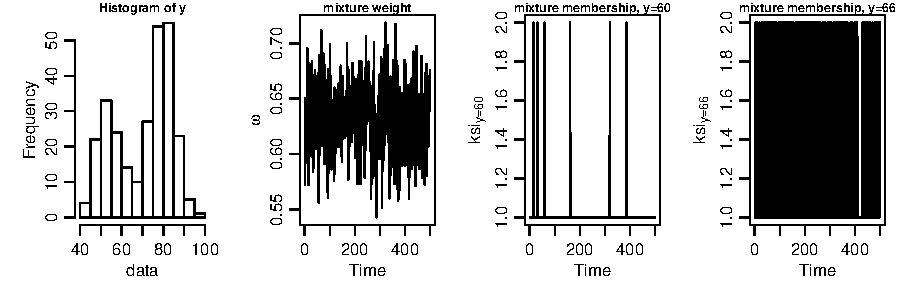
\includegraphics[width=4in]{plots/mixture-faithful}

\end{itemize}
}




\frame{
\sffamily
\frametitle{Auxiliary variables}
\begin{itemize}
\item {\bf Example (Probit regression, \citealp{AlCh93}):  }  For $i=1, \ldots, n$ let $y_i \mid \theta_i \sim \Ber \left( \theta_i \right)$ where $\Phi^{-1}\left( \theta_i \right) = \bfx_i^T \bfbeta$, $\bfx_i$ is a vector of known  regressors and $\bfbeta$ is a vector of regression coefficients with $\bfbeta \sim \normal(\mathbf{0}, \bfSigma)$.

\vspace{1mm}

In this case introduce auxiliary variables $z_1, \ldots, z_n$ such that
\begin{align*}
z_{i} \mid \bfbeta &\sim \normal(\bfx_i^T\bfbeta, 1)   &   
%
y_{i} &= \begin{cases} 
1 & z_i \ge 0  \\
0 & z_i < 0
\end{cases}
\end{align*}

The full conditional for $\bfbeta$ is Gaussian, while the full conditional of $z_i$ is a truncated normal.  A slight improvement can be obtained if instead of working with $z_i \mid \bfbeta$ you work with $z_i | z_{-i}$ (this is an example of marginalization, see \citealp{holmes2006bayesian}).
\end{itemize}
}





\frame{
\sffamily
\frametitle{Auxiliary variables}
\begin{itemize}
\item {\bf Example (Robust regression):}   Consider the robust regression model
\begin{align*}
y_i &= \bfx_i^T \bfbeta + \sigma \epsilon_i ,   & \epsilon &\sim t_{\nu}  ,     &    i=1, \ldots, n.
\end{align*}
where $\bfbeta \sim \normal(\mathbf{0}, \bfSigma^2)$, $\sigma^2 \sim \IGam(a, c)$ and $\nu \sim p(\nu)$.  

\vspace{1mm}

It is well known that the Student $t$ distribution can be written as a scale mixture of normals.  Accordingly, introduce auxiliary variables $\lambda_1, \ldots, \lambda_n$ such that
\begin{align*}
y_i \mid \bfbeta, \sigma^2, \lambda_i &\sim \normal \left( \bfx_i^T \bfbeta, \frac{\sigma^2}{\lambda_i} \right) ,    &   \lambda_i &\sim \Gam\left( \frac{\nu}{2}, \frac{\nu}{2} \right) .
\end{align*}

Including $\lambda_1, \ldots, \lambda_n$ in the model makes the full conditional for $\bfbeta$ a Gaussian and the full conditional for $\sigma^2$ an inverse Gamma.  On the other hand, the full conditional for $\lambda_i$ is another Gamma, while $\nu$ needs to be sampled using a MH step (preferably from the unaugmented model!).
\end{itemize}
}









\frame{
\sffamily
\frametitle{Adaptive MCMC algorithms}
\begin{itemize}
\item  As our Metropolis examples illustrate, one of the main challenges associated with designing MH  algorithms is selecting the proposal distribution.

\item In particular, concentrate on (Gaussian) random-walk MH algorithms, where the problem is how to select the variance-covariance matrix.  What we have done so far requires a lot of back and forth!

\item Is there a way in which we can create a ``self-tuning'' algorithm?  This is the main thrust behind \alert{adaptive MCMC algorithms}!!!
\end{itemize}
}



\frame{
\sffamily
\frametitle{Adaptive MCMC algorithms}
\begin{itemize}
\item A simple yet powerful idea (at least for elliptical posteriors):  start with a potentially very bad covariance matrix and, after the algorithm has been running for a while, switch to different proposal that uses the previous values of the chain to estimate $\Cov( \bftheta \mid \bfy)$ (just as we did when we manually tuned the chain).

\item This is particularly useful when $\dim\{ \bftheta \} = d$ is large!

\item  The main conceptual issue with this approach is that using the whole history of the chain to create a proposal means that we are not working with a Markov chain anymore (or, at least, not with a time-homogenous one), so the theory we discussed so far cannot be used to ensure that the algorithm actually converges to the desired equilibrium distribution.
\end{itemize}
}




\frame{
\sffamily
\frametitle{Adaptive MCMC algorithms}
\begin{itemize}
\item {\bf Example (taken from \citealp{RoRo:09} and \citealp{haario2001adaptive}):  }  Consider a target distribution $\normal(\mathbf{0}, \bfM \bfM^T)$ where the entries of $\bfM$ have been randomly generated from standard normal distribution.

\vspace{1mm}

We consider the case $d=\dim\{ \bftheta \} = 10$.  For the first $20,000$ iterations, the proposal distribution is fixed and corresponds to a normal distribution, $q(\vartheta \mid \theta) = \normal\left( \vartheta \mid \theta, \frac{0.1^2}{d} \mathbf{I} \right)$.  After that point, the proposal becomes a mixture
$$
q(\vartheta \mid \theta) = (1- \beta) \normal \left(\vartheta \mid \theta, \frac{2.38^2}{d} \bfSigma_b \right) + \beta \normal\left(\vartheta \mid \theta, \frac{0.1^2}{d} \mathbf{I} \right)
$$
where $\bfSigma_b$ is the current empirical estimate of the covariance of the target distribution (computed on the basis of the previous $b-1$ iterations of the chain), and $\beta > 0$ is a (small) constant.
\end{itemize}
}





\frame{
\sffamily
\frametitle{Adaptive MCMC algorithms}
\begin{itemize}
\item {\bf Example (taken from \citealp{RoRo:09} and \citealp{haario2001adaptive}, cont):  }  The algorithm is implemented in the file \texttt{adaptive1.R}, which allows you to run the algorithm using only the ``default'', only the ``optimal'', and the adaptive proposal.  The graphs below show the trace plots for the first component of $\bftheta$. 

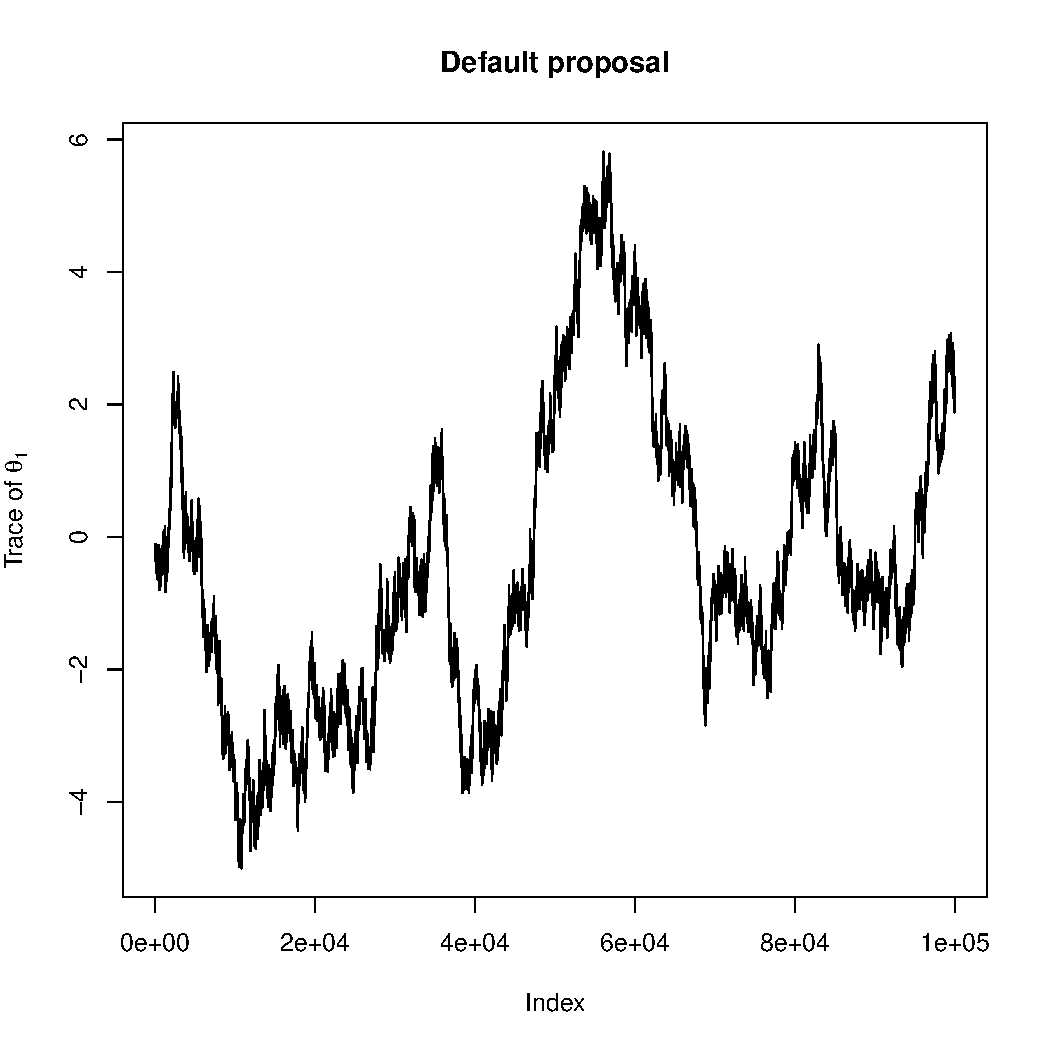
\includegraphics[height=3.3cm,angle=0]{plots/adap_trace_def.pdf}
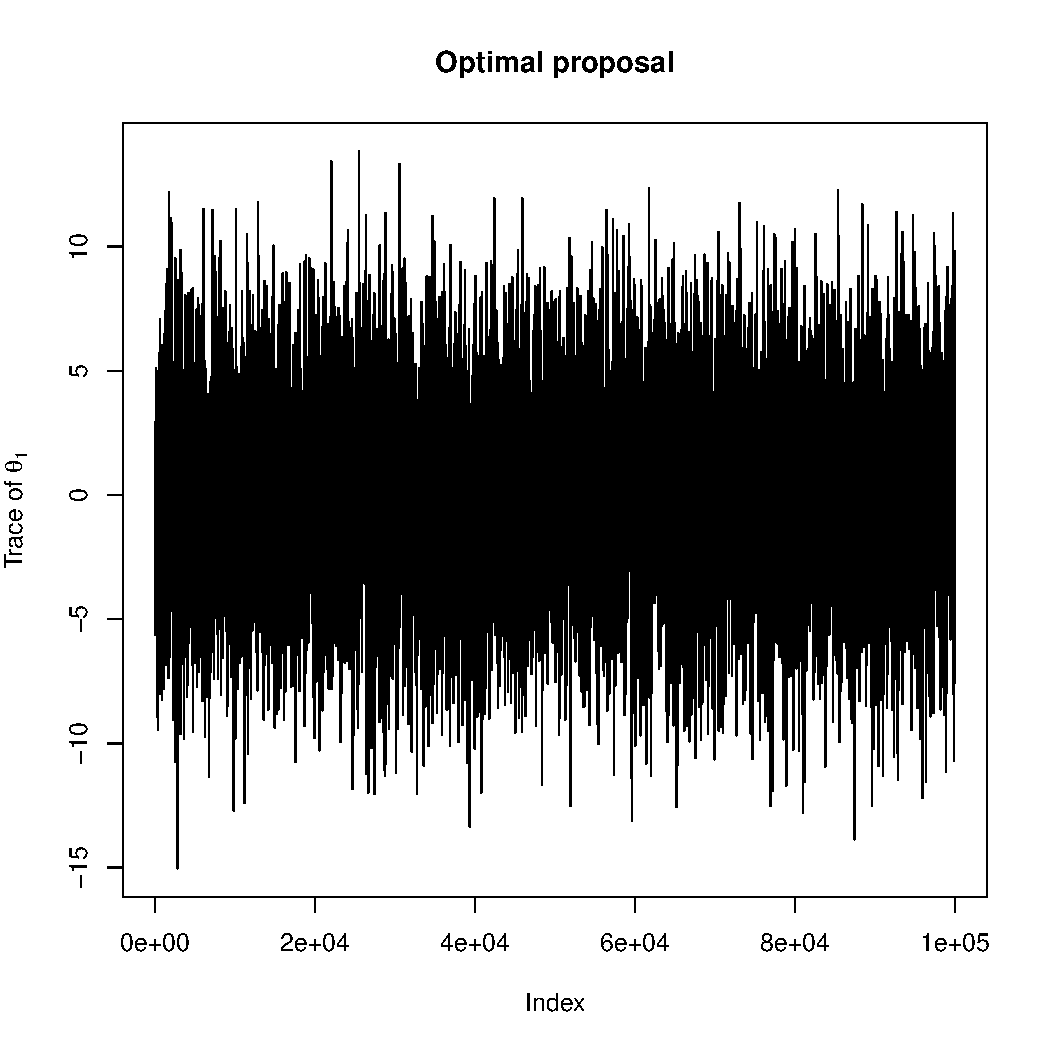
\includegraphics[height=3.3cm,angle=0]{plots/adap_trace_opt.pdf}
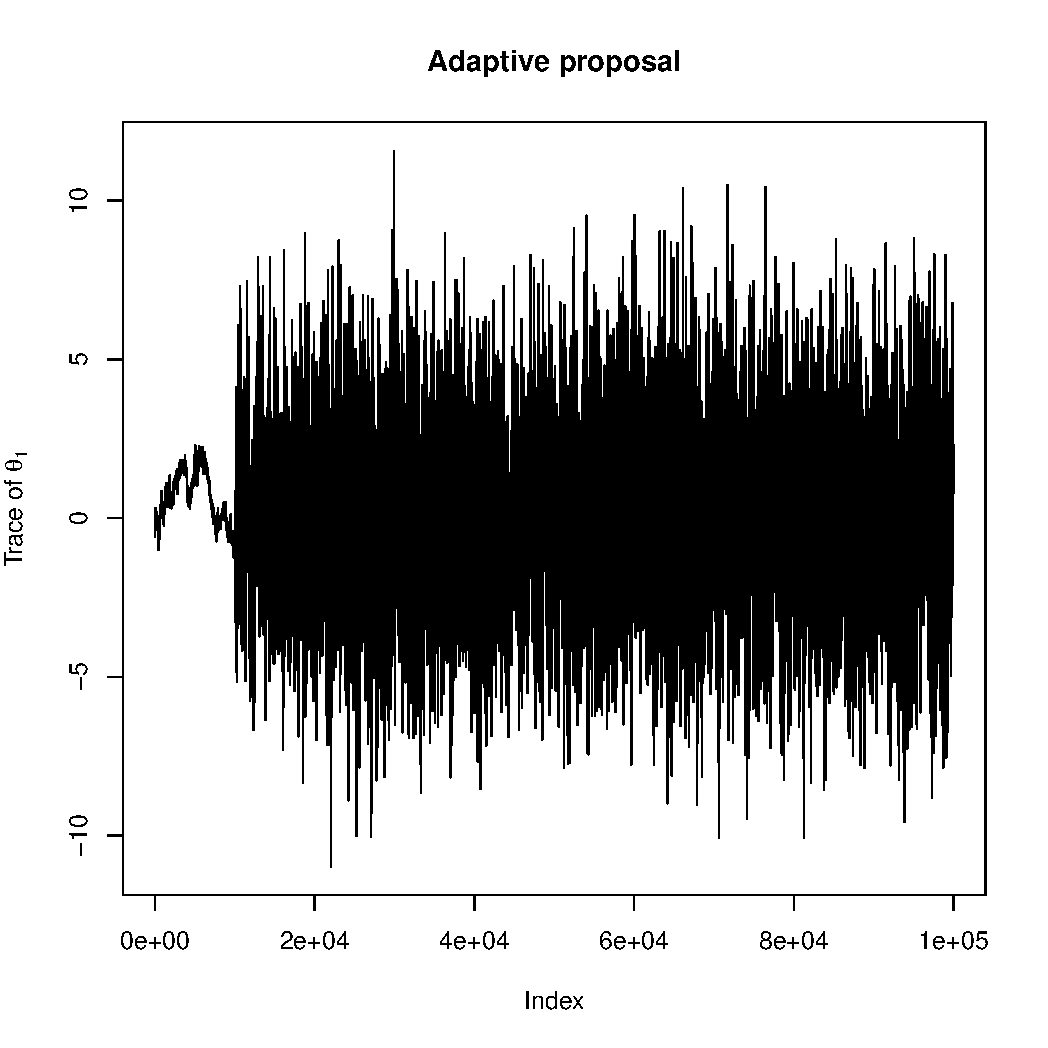
\includegraphics[height=3.3cm,angle=0]{plots/adap_trace_adp.pdf}


\end{itemize}
}




\frame{
\sffamily
\frametitle{Adaptive MCMC algorithms}
\begin{itemize}
\item {\bf Example (taken from \citealp{RoRo:09} and \citealp{haario2001adaptive}, cont):  }    The graphs below show the acf functions for the first component of $\bftheta$.

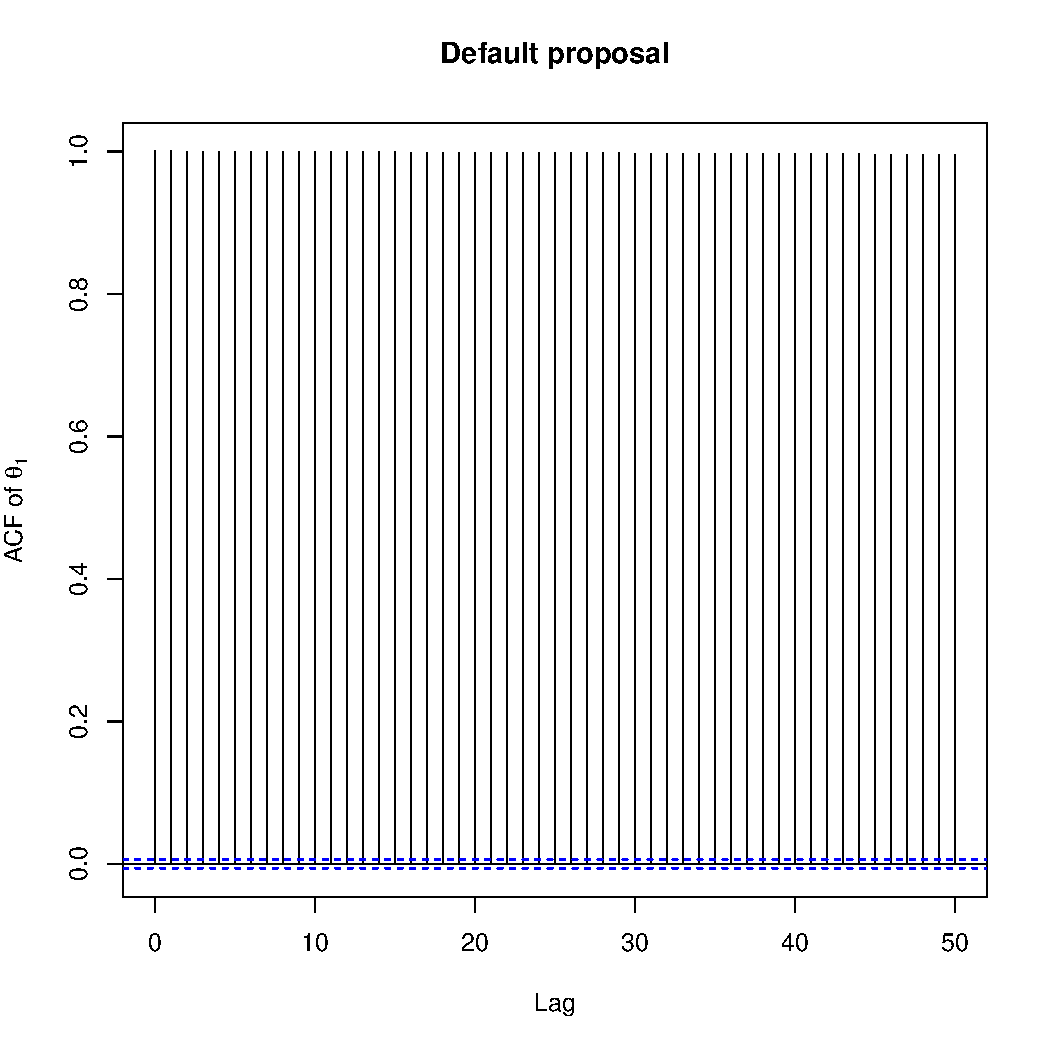
\includegraphics[height=3.3cm,angle=0]{plots/adap_acf_def.pdf}
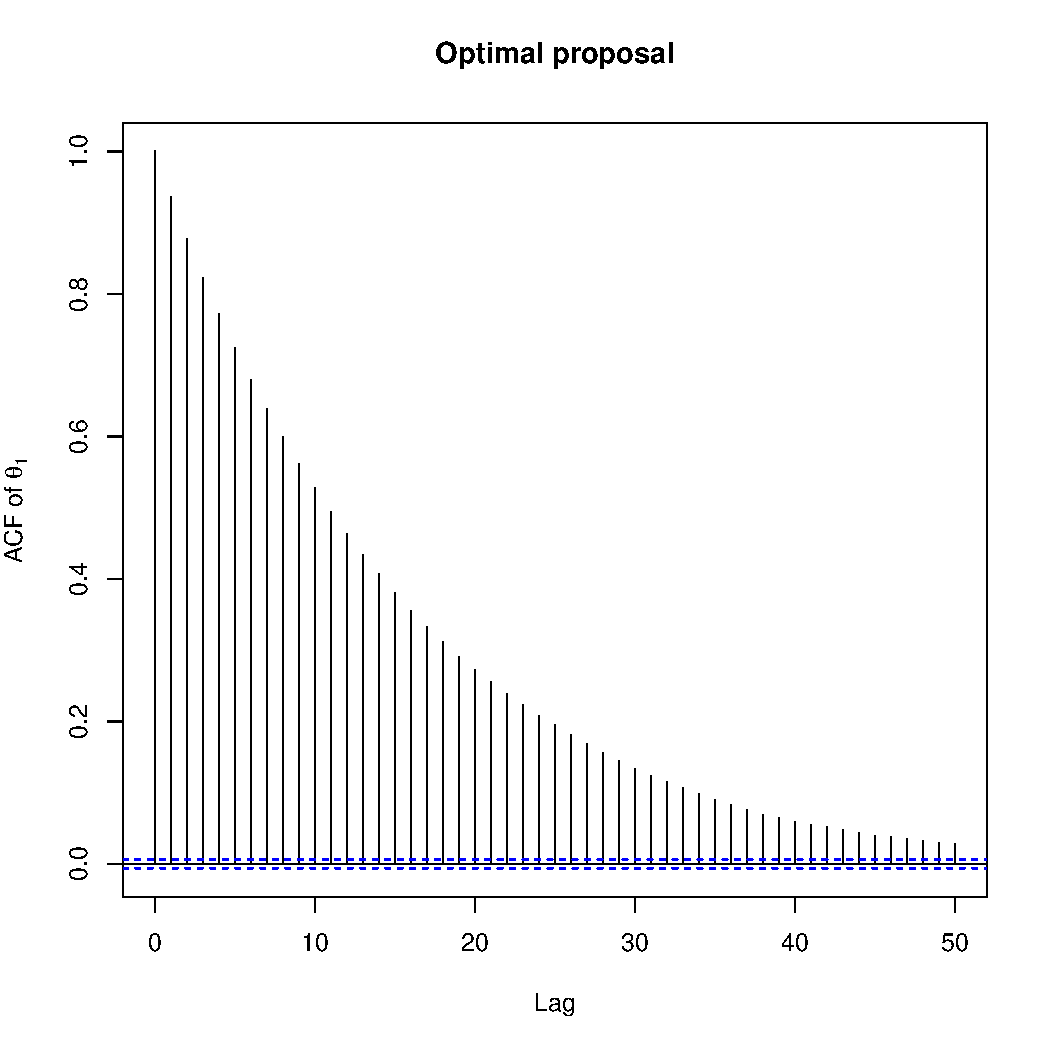
\includegraphics[height=3.3cm,angle=0]{plots/adap_acf_opt.pdf}
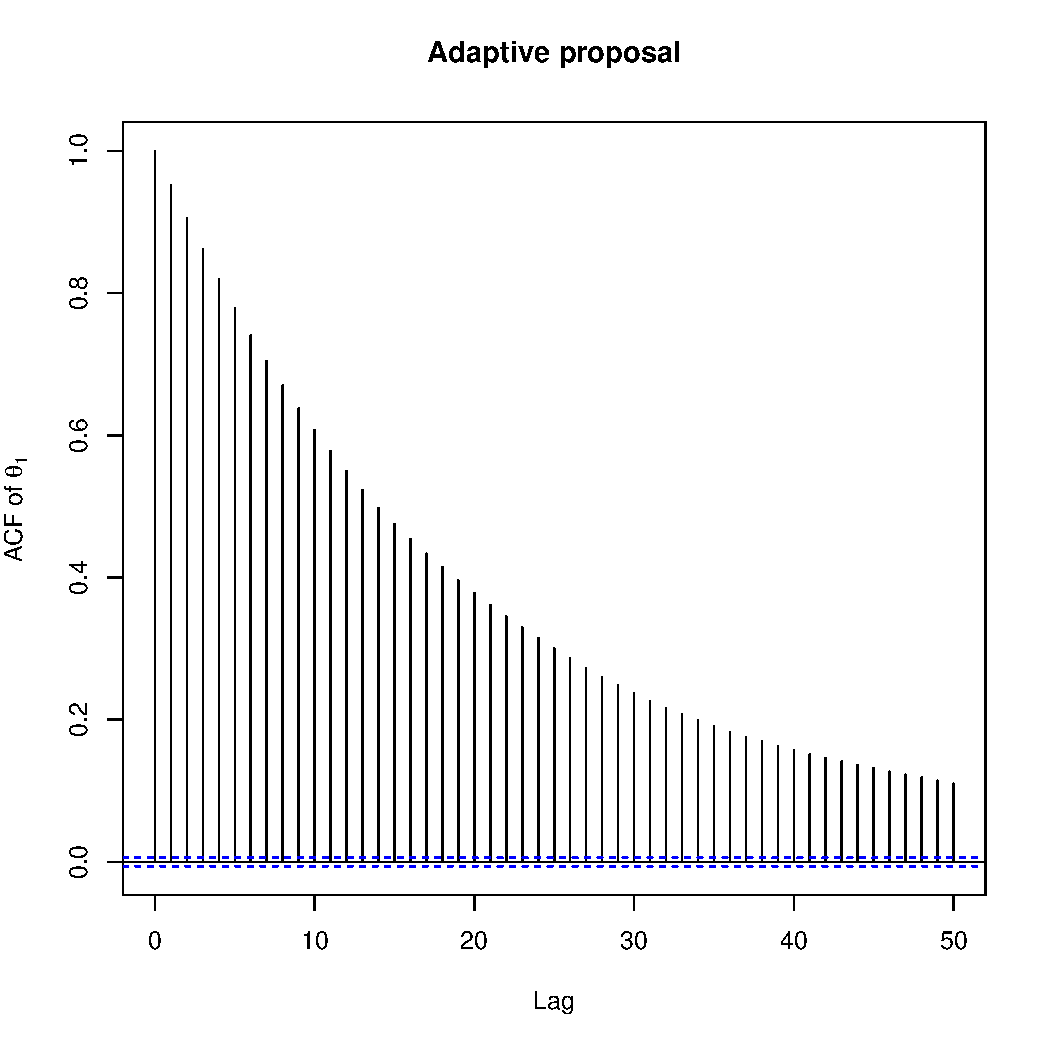
\includegraphics[height=3.3cm,angle=0]{plots/adap_acf_adp.pdf} \\


Acceptance rates are 0.964, 0.264, and 0.260.  The effective sample sizes in the last two cases are 3096 and 3200.
\end{itemize}
}



\frame{
\sffamily
\frametitle{Adaptive MCMC algorithms}
\begin{itemize}
\item {\bf Example (taken from \citealp{RoRo:09} and \citealp{haario2001adaptive}, cont):  }  

Some things to consider:
\begin{itemize}
\item The use of $20,000$ ``preliminary'' samples and a ``default'' variance $ \frac{0.1^2}{d} \mathbf{I}$ are totally ad-hoc.

\item More recent schemes (including that in NIMBLE) adapt on the fly (e.g., every 100 iterations), averaging the current proposal covariance with the estimated posterior covariance from recent iterations.

\item Adaptive univariate schemes simply adjust the proposal scale.

\end{itemize}
\end{itemize}
}

\frame{
\sffamily
\frametitle{Adaptive MCMC algorithms}

NIMBLE's adaptive MCMC
\begin{itemize}
\item NIMBLE's default scalar and block Metropolis samplers use adaptation. 
\item Users can set the initial proposal scale / covariance.
\item Current scheme can sometimes perform very poorly when the scales of initial proposal covariance and the posterior covariance are very different.
\begin{itemize}
\item We plan to roll out a fix for this in the next release.
\end{itemize}
\end{itemize}
}

\begin{frame}[fragile]
\sffamily
\frametitle{Adaptive MCMC algorithms}

\begin{itemize}
\item {\bf Example (Nonlinear binomial regression):} in \texttt{mh-bliss.R} we have NIMBLE code for non-adaptive (theoretical proposal covariance) and adaptive blocked and univariate Metropolis sampling. 
\begin{center}
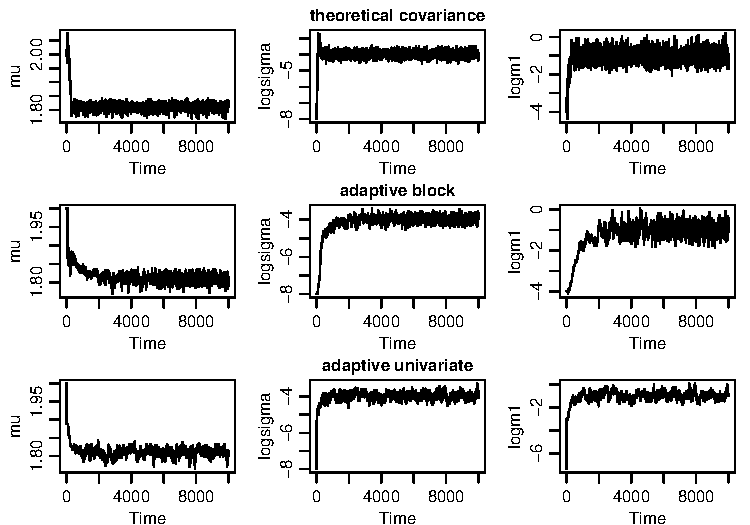
\includegraphics[width=3.0in]{plots/adaptive-bliss}
\end{center}
\end{itemize}

\end{frame}








\frame{
\sffamily
\frametitle{Hamiltonian Monte Carlo}
\begin{center}
\begin{tabular}{lr}
\begin{minipage}{5.1cm}
\begin{itemize}
\item One of the main challenges for all the previous MCMC methods is dealing with non-elliptical posteriors.

\item We would like to exploit the local geometry of the distribution.

\item HMC methods allow us to do precisely that!
\end{itemize}
\end{minipage}
%&
\begin{minipage}{5.3cm}
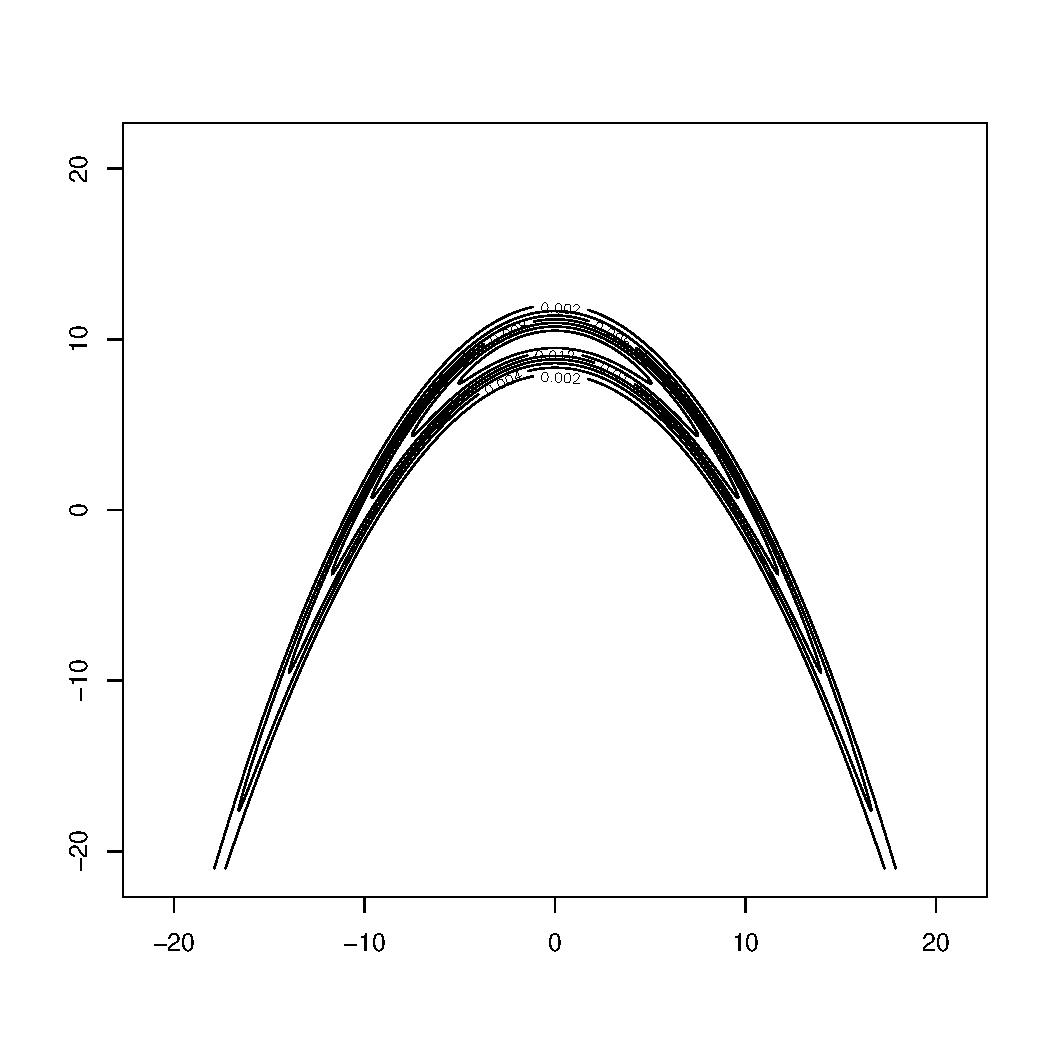
\includegraphics[width=5.2cm,angle=0]{plots/banana_density.pdf}
\end{minipage}
\end{tabular}
\end{center}
}





\frame{
\sffamily
\frametitle{Hamiltonian Dynamics}
\begin{center}
\vspace{-1mm}
\begin{tabular}{lr}
\hspace{-10mm}
\begin{minipage}{6.0cm}
\begin{itemize}
{\small \item The Hamiltonian function $H$ describes the time evolution of a dynamical system (e.g., a spring).

\item For Bayesian inference we are interested mainly in Hamiltonians of the form
$$
H(\bftheta, \bfphi) = U(\bftheta) + K(\bfphi)
$$
where $\bftheta \in \reals^d$ is the ``position'', $\bfphi \in \reals^d$ is the ``momentum'', $U$ is the potential energy and $K$ is the kinetic energy.}
\end{itemize}
\end{minipage}
%&
\begin{minipage}{4cm}
%\vspace{-8mm}
%\hspace{-8mm}
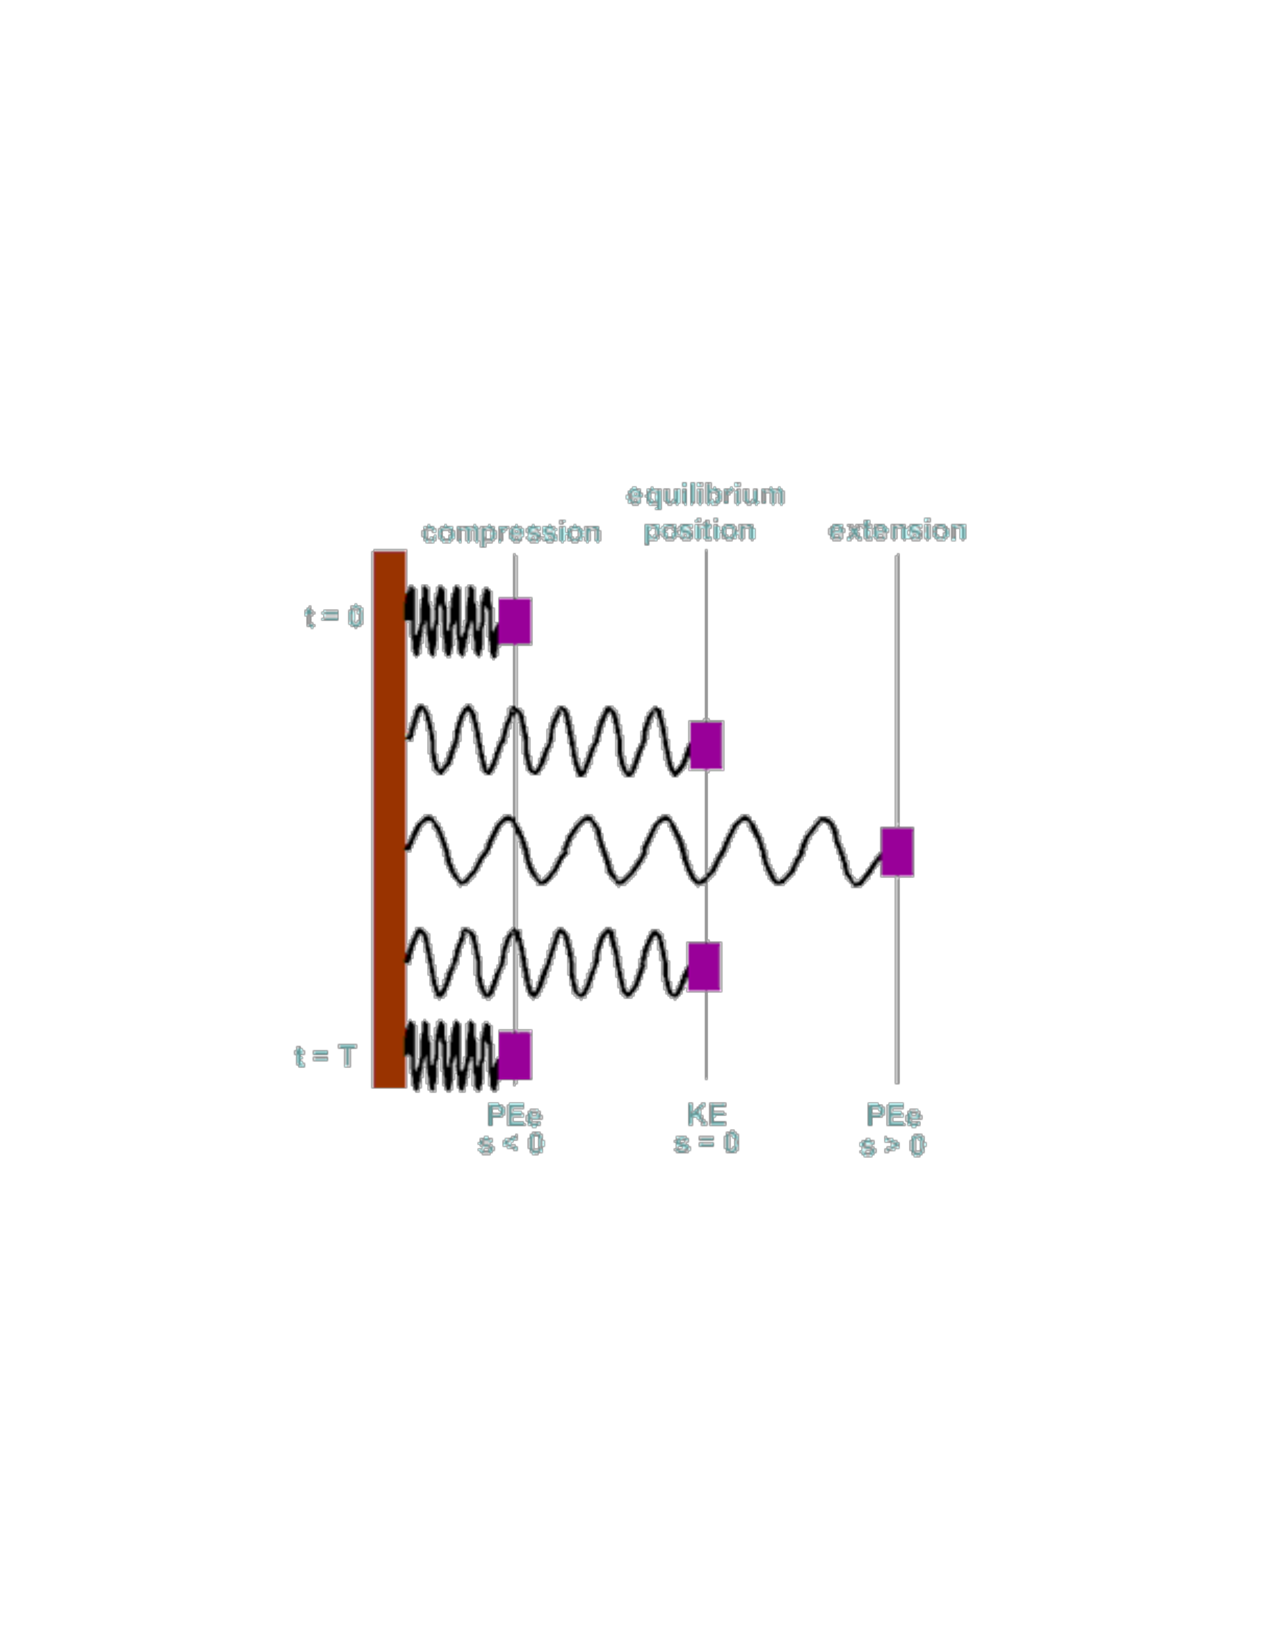
\includegraphics[width=5cm,angle=0]{plots/spring2.pdf}
\end{minipage}
\end{tabular}
\end{center}
}



\frame{
\sffamily
\frametitle{Hamiltonian Dynamics}
\begin{itemize}
\item For our purpose, the ``position'' $\bftheta$ corresponds to our parameters of interest and
$$
U(\bftheta) = -\log \left\{ p(\bftheta \mid \bfy) \right\}.
$$

\item The momemtun $\bfphi$ corresponds to auxiliary variables, and the form of the kinetic energy is arbitrary (as long as it is the negative of the logarithm of a well-defined density).  Often $\bfphi \sim \normal(\mathbf{0}, \mathbf{M})$ with $\mathbf{M} = \diag\{ m_1, \ldots, m_K \}$, so
$$
K(\bfphi) = \frac{1}{2} \bfphi^T\mathbf{M}\bfphi = \frac{1}{2} \sum_{k=1}^{d} m_k\phi_k^2.
$$
Can be interpreted as the kinetic energy available to $d$ springs (with constants $m_1, \ldots, m_K$) that have been stretched $\phi_1, \ldots, \phi_K$ units away from their equilibrium position.
\end{itemize}
}





\frame{
\sffamily
\frametitle{Hamiltonian Dynamics}
\begin{itemize}
\item The time evolution of the system is uniquely defined by Hamilton's equations,
\begin{align*}
\frac{\dd \bftheta}{\dd t} &= - \frac{\partial H}{\partial \bfphi}  ,    &    \frac{\dd \bfphi}{\dd t} &=  \frac{\partial H}{\partial \bftheta}
\end{align*} 

\item The Hamiltonian remains invariant as time evolves, i.e., 
$$
\frac{\dd H}{\dd t} = 0 .
$$
(easy to show using Hamilton's equations and the chain rule).  

\item \alert{The dynamics induced by the Hamiltonian equations are reversible.  They also preserve volume in the $(\bftheta, \bfphi)$ space (which implies a unit Jacobian).}
\end{itemize}
}



\frame{
\sffamily
\frametitle{Hamiltonian Dynamics and MCMC}
The path forward should be clear
\begin{itemize}
\item We want to build an MCMC on the augmented space $(\bftheta, \bfphi)$ with stationary distribution
$$
p(\bftheta, \bfphi) \propto \exp\left\{ - U(\bftheta) - K(\bfphi) \right\}
$$
where $U(\bftheta) = p(\bftheta \mid \bfy)$ that uses Hamilton's dynamics (which are reversible and volume-preserving) to generate proposals.

\item If we can simulate the dynamic over time exactly, then this is a valid MH proposal, and will always be accepted (because of the time invariance of the Hamiltonian).

\item In practice we can only simulate the dynamics approximately by discretizing time.  If we do it carefully, the discretized dynamics will still be reversible and volume-preserving (although only be approximately invariant ...).
\end{itemize}
}






\frame{
\sffamily
\frametitle{Discretizing the Hamiltonian Dynamics}
\begin{itemize}
\item Euler's method (step size $\epsilon$):
{\small \begin{align*}
\phi_i(t + \epsilon) &= \phi_i(t) + \epsilon \frac{\dd \phi_i}{\dd t}(t) = \phi_i(t) - \epsilon \frac{\partial U}{\partial \theta_i}(\bftheta(t)) \\
\theta_i(t + \epsilon) &= \theta_i(t) + \epsilon \frac{\dd \theta_i}{\dd t}(t) = \theta_i(t) + \epsilon \frac{\partial K}{\partial \phi_i}(\bfphi(t))
\end{align*}}
Discretized dynamics are not necessarily reversible.

\item \alert{Better:}  ``Leapfrog method'' (step size $\epsilon$):
{\small \begin{align*}
\phi_i(t + \epsilon/2) &=  \phi_i(t) - \frac{\epsilon}{2} \frac{\partial U}{\partial \theta_i}(\bftheta(t)) \\
\theta_i(t + \epsilon) &= \theta_i(t) + \epsilon \frac{\partial K}{\partial \phi_i}(\bfphi(t + \epsilon/2)) \\
\phi_i(t + \epsilon) &=  \phi_i(t + \epsilon/2) - \frac{\epsilon}{2} \frac{\partial U}{\partial \theta_i}(\bftheta(t + \epsilon))
\end{align*}}

\item \alert{Even Better:}  Multiple steps of ``Leapfrog''.
\end{itemize}
}









\frame{
\sffamily
\frametitle{The Hamiltonian Monte Carlo algorithm}
Discretized Hamiltonian trajectories for $H(\theta, \phi) = \theta^2 + \phi^2$ using the leapfrog method.  Left panel corresponds to $\epsilon = 0.3$ and the right to $\epsilon = 1.2$.
\begin{center}
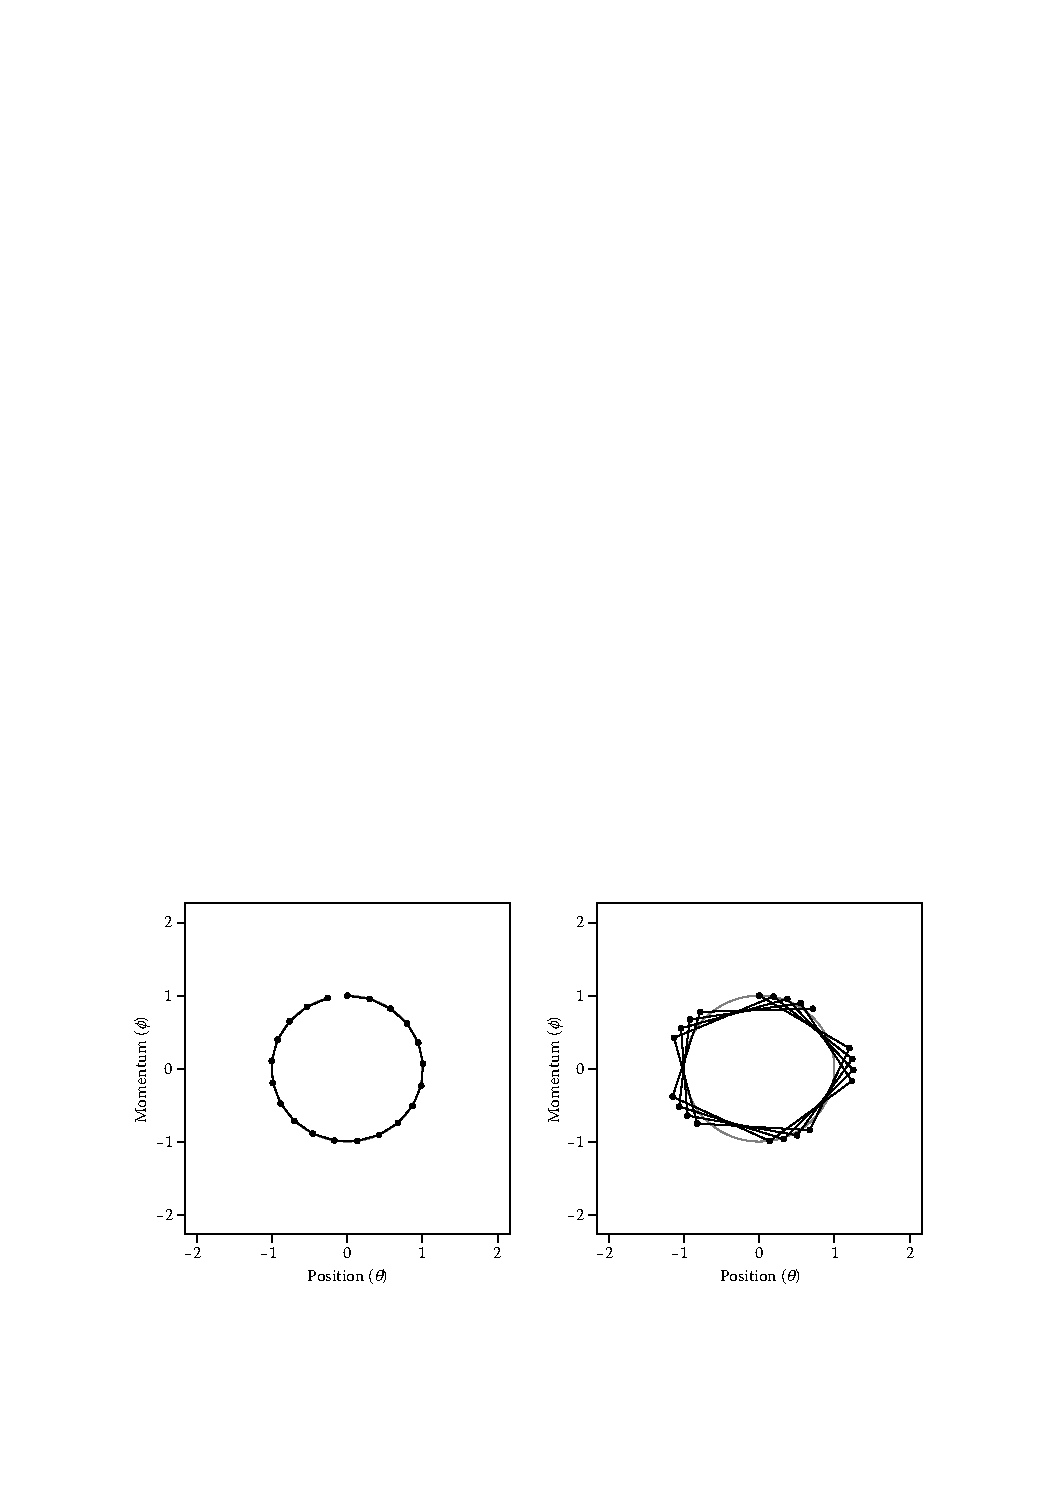
\includegraphics[width=9cm,angle=0]{plots/hamiltonian_neil.pdf}
\end{center}

{\hfill \scriptsize Taken from \cite{neal2011mcmc}.}
}






\frame{
\sffamily
\frametitle{The Hamiltonian Monte Carlo algorithm}
\begin{enumerate}
{\scriptsize \item Generate $\bfphi^{(s)} \sim q$, where $q \propto \exp \left\{ - K(\bfphi) \right\}$.
\item Initialize $\bfvarphi^{(s)} = \bfphi^{(s)}$ and $\bfvartheta^{(s)} = \bftheta^{(s)}$
\item Update $\bfvarphi^{(s + 1/(L+1))} = \bfvarphi^{(s)} - \frac{\epsilon}{2} \frac{\partial U}{\partial \theta_i}(\bftheta^{(s)})$.
\item For $l = 1, \ldots, L-1$
\begin{enumerate}
\item Update $\bfvartheta^{(s + l/L)} = \bfvartheta^{(s + (l-1)/L)} + \epsilon\frac{\partial K}{\partial \phi_i}(\bfvarphi^{(s + l/(L+1))})$.
\item Update $\bfvarphi^{(s + (l+1)/(L+1))} = \bfvarphi^{(s + l/(L+1))} - \epsilon\frac{\partial U}{\partial \theta_i}(\bfvartheta^{(s + l/L))})$.
\end{enumerate}
\item Update $\bfvartheta^{(s + 1)} = \bfvartheta^{(s + (L-1)/L)} + \epsilon\frac{\partial K}{\partial \phi_i}(\bfvarphi^{(s + L/(L+1))})$.
\item Update $\bfvarphi^{(s + 1)} = \bfvarphi^{(s - L/(L+1))} - \frac{\epsilon}{2} \frac{\partial U}{\partial \theta_i}(\bfvartheta^{(s + 1)})$.
\item Set 
$$
\bftheta^{(s+1)} = \begin{cases} 
\bfvartheta^{(s+1)}  & \mbox{with prob. } \rho(\bftheta^{(s)}, \bfphi^{(s)}, \bfvartheta^{(s+1)}, \bfvarphi^{(s+1)})  \\
\bftheta^{(s)}  & \mbox{with prob. } 1 - \rho(\bftheta^{(s)}, \bfphi^{(s)}, \bfvartheta^{(s+1)}, \bfvarphi^{(s+1)})
\end{cases}$$
where
\begin{multline*}
\rho(\bftheta^{(s)}, \bfphi^{(s)}, \bfvartheta^{(s+1)}, \bfvarphi^{(s+1)}) = \\
%
\min\left\{ 1, \exp\left\{ U\left(\bftheta^{(s)}\right) - U\left(\bfvartheta^{(s+1)}\right) + K\left(\bfphi^{(s)}\right) - K\left(-\bfvarphi^{(s+1)}\right) \right\} \right\}
\end{multline*}
}
\end{enumerate}
}





\frame{
\sffamily
\frametitle{The Hamiltonian Monte Carlo algorithm}
\begin{itemize}
\item {\bf Example (sampling from the Cauchy distribution):  }  Consider using a Hamiltonian Monte Carlo algorithm to sample from a Cauchy distribution $p(\theta) = \frac{1}{\pi (1 + \theta^2)}$.  We use a Gaussian distribution for the momentum, so
\begin{align*}
U(\theta) &= - \log p(\theta) = \log \left\{ 1 + \theta^2 \right \}  ,   &  K(\phi) &= \frac{\phi^2}{2}  .
\end{align*}
\item Hence, we have
\begin{align*}
\frac{\partial U}{\partial \theta} &= \frac{2\theta}{ 1 + \theta^2}  ,  &  \frac{\partial K}{\partial \phi} &= \phi  .
\end{align*}
\end{itemize}
}





\frame{
\sffamily
\frametitle{The Hamiltonian Monte Carlo algorithm}
\begin{itemize}
\item {\bf Example (sampling from the Cauchy distribution, cont):}  If we take a single step ($L=1$) of length $\epsilon$ 
$$
\theta^{(p)} = \theta^{(c)} \left\{ 1 - \frac{\epsilon^2}{1 + \left( \theta^{(p)} \right)^2} \right\} + \epsilon \phi^{(c)}
$$
where $\phi^{(c)} \sim \normal(0,1)$.

\item This looks similar to what you would get from a random walk proposal with standard deviation $\epsilon$, $\theta^{(p)} = \theta^{(c)} + \epsilon \omega$ where $\omega \sim \normal(0,1)$.

\item However, there are some important differences!
\end{itemize}
}





\frame{
\sffamily
\frametitle{The Hamiltonian Monte Carlo algorithm}
\begin{itemize}
\item {\bf Example (sampling from the Cauchy distribution, cont):}  Suppose $\theta^{(p)} = -3$.

\item The random walk proposal has the same probability of proposing a value to the right of $\theta^{(p)}$ as it does a value to the left.

\item For small $\epsilon$ we have $\left\{ 1 - \frac{\epsilon^2}{1 + \left( \theta^{(p)} \right)^2} \right\} \in [0,1]$.  Hence, the Hamiltonian MH algorithm has a higher probability of proposing value to the right of $-1$ than values to its left.  This is what you would intuitively would like to do!

\item A similar argument applies for positive values of $\theta^{(p)}$.
\end{itemize}
}





\frame{
\sffamily
\frametitle{The Hamiltonian Monte Carlo algorithm}
\begin{itemize}
\item {\bf Example (sampling from the Cauchy distribution, cont):}  Suppose $\theta^{(c)} = -3$ and $\epsilon = 1$
\begin{center}
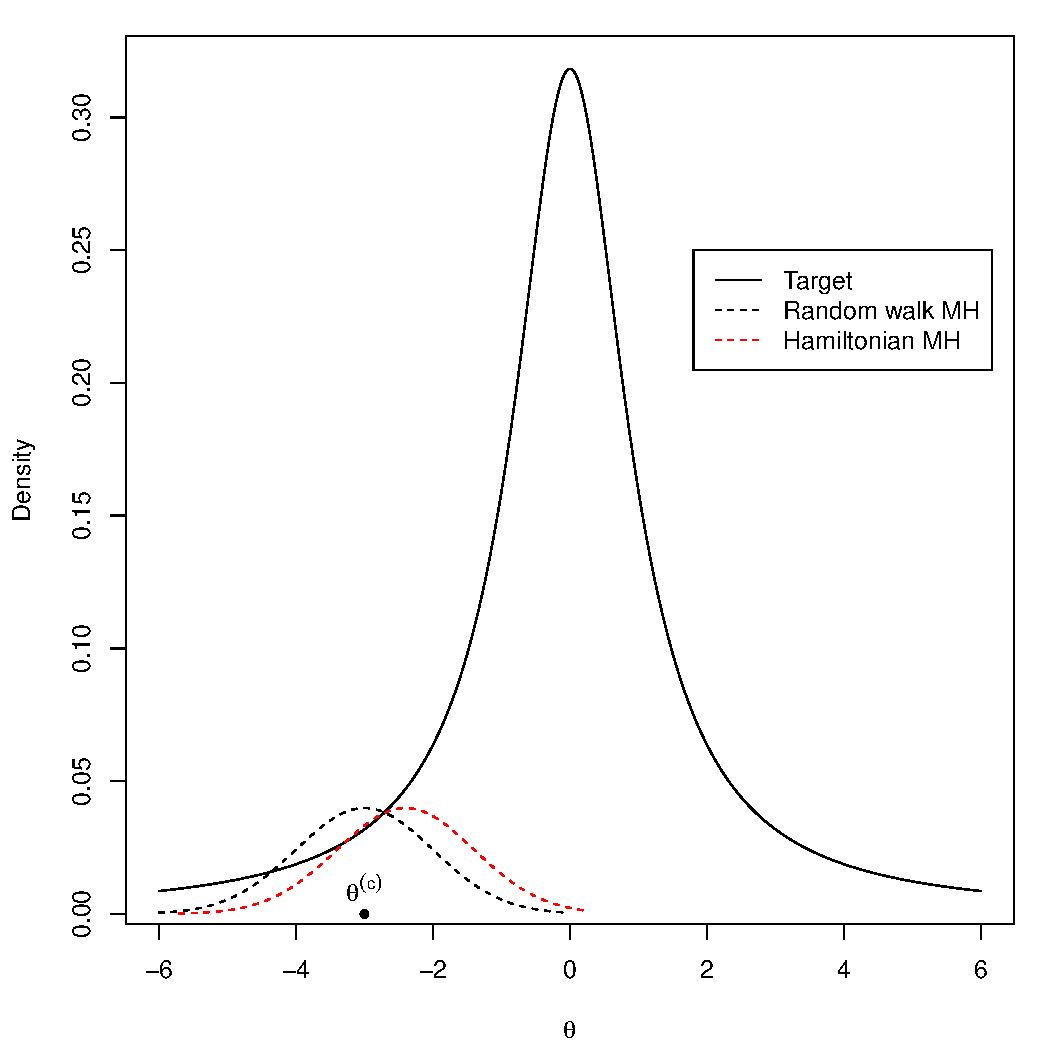
\includegraphics[width=6cm,angle=0]{plots/hamiltoniancauchy.pdf}
\end{center}
\end{itemize}
}








\frame{
\sffamily
\frametitle{The Hamiltonian Monte Carlo algorithm}
\hspace{-3mm}
\begin{center}
\begin{tabular}{lr}
\begin{minipage}{5.6cm}
{\small {\bf Example (bivariate normal target):}  Consider sampling from the bivariate normal distribution
$$
\left(\begin{matrix}
\theta_1  \\
\theta_2 \end{matrix}\right) \sim \normal \left(
\left(\begin{matrix}
15  \\
45 \end{matrix}\right) ,
\left(\begin{matrix}
1  &  0.95  \\
0.95  & 1 \end{matrix}\right)
\right)
$$}
using both a Hamiltonian Monte Carlo and a bivariate random walk.
\end{minipage}
&
\begin{minipage}{5.6cm}
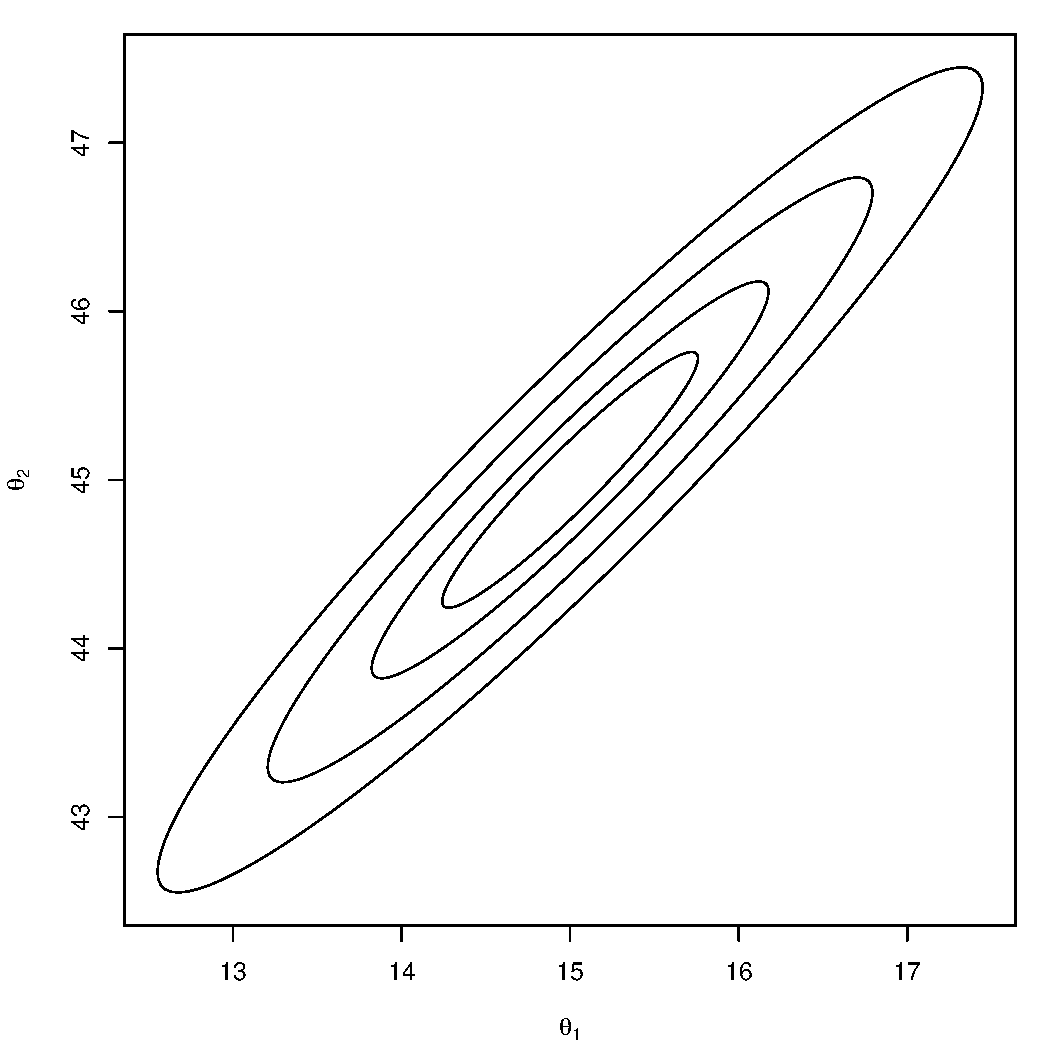
\includegraphics[height=4.5cm,angle=0]{plots/bivariatenormalhighcor.pdf}
\end{minipage}
\end{tabular}
\end{center}
}









\frame{
\sffamily
\frametitle{The Hamiltonian Monte Carlo algorithm}
\begin{itemize}
\item {\bf Example (bivariate normal target, cont):}  For the Hamiltonian algorithm we use independent Gaussian distributions for the momentum variables $\phi_1$ and $\phi_2$.  The gradients are
\begin{align*}
\nabla U (\bftheta) &= \left(\begin{matrix}
1  &  0.95  \\
0.95  & 1 \end{matrix}\right)^{-1} \bftheta    &   \nabla K(\bfphi) &= \bfphi
\end{align*}

\item For the random walk Metropolis algorithm, we use an optimal bivariate Gaussian proposal
$$
\bfvartheta^{(s+1)} \mid \bftheta^{(s)} \sim \normal \left(  \bftheta^{(s)} , 
\frac{2.38^2}{2} \left(\begin{matrix}
1  &  0.95  \\
0.95  & 1 \end{matrix}\right)
\right)
$$
\item Code in \texttt{hamiltonian\_bivariatenormal.R}.
% Acceptance rate around 36%
% \texttt{hamiltonian\_bivariatenormal.R}
\end{itemize}
}






\frame{
\sffamily
\frametitle{The Hamiltonian Monte Carlo algorithm}
\begin{tabular}{cc}
{\small Random walk}   &   {\small Hamiltonian}   \\
{\small Acceptance rate 36\%}   &   {\small Acceptance rate  89\%} \\
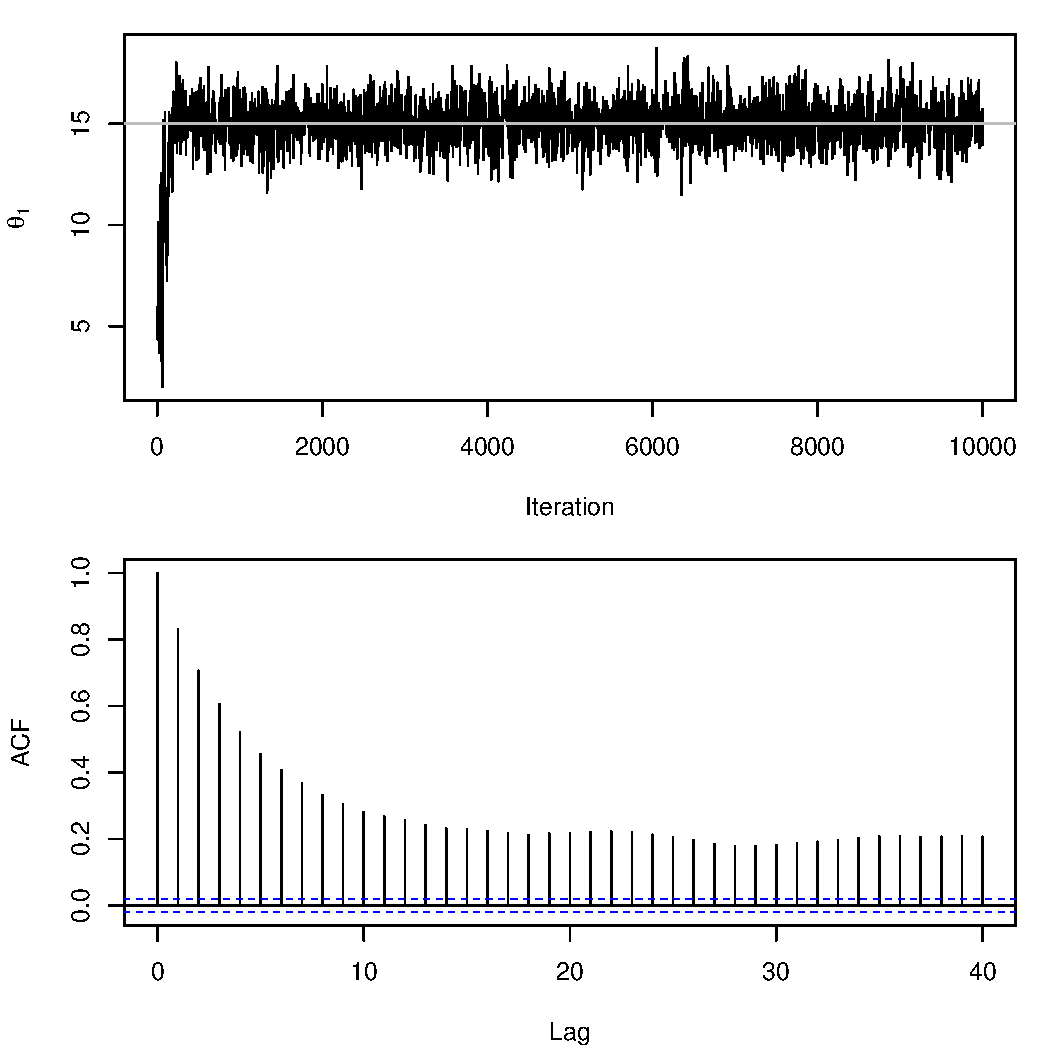
\includegraphics[height=4.9cm,angle=0]{plots/bivariatenormal_RW.pdf}  &  
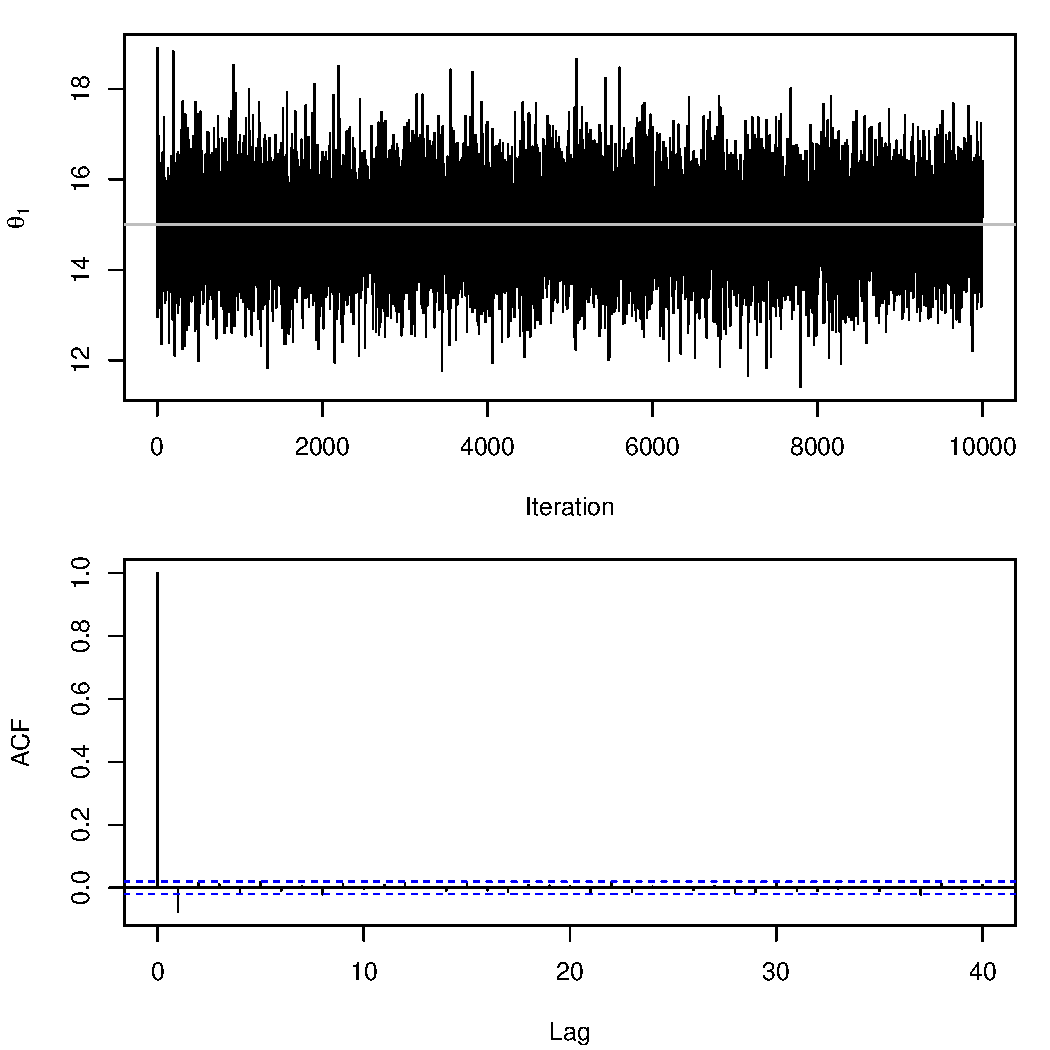
\includegraphics[height=4.9cm,angle=0]{plots/bivariatenormal_hamiltonian.pdf}
\end{tabular}
}







\frame{
\sffamily
\frametitle{Hamiltonian Dynamics}
\begin{center}
\begin{tabular}{lr}
\vspace{-3mm} \begin{minipage}{5.4cm}
\begin{itemize}
{\small \item Hamiltonian algorithms can be useful in moving you across modes because proposals happen (approximately) along constant-energy contours.
\item For example, consider sampling from a mixture of two normals
$$
0.5 \normal(-2,1) + 0.5 \normal(2,1)
$$
using a standard Gaussian distribution for the momentum variables.
}
\end{itemize}
\end{minipage}
&
\begin{minipage}{5.6cm}
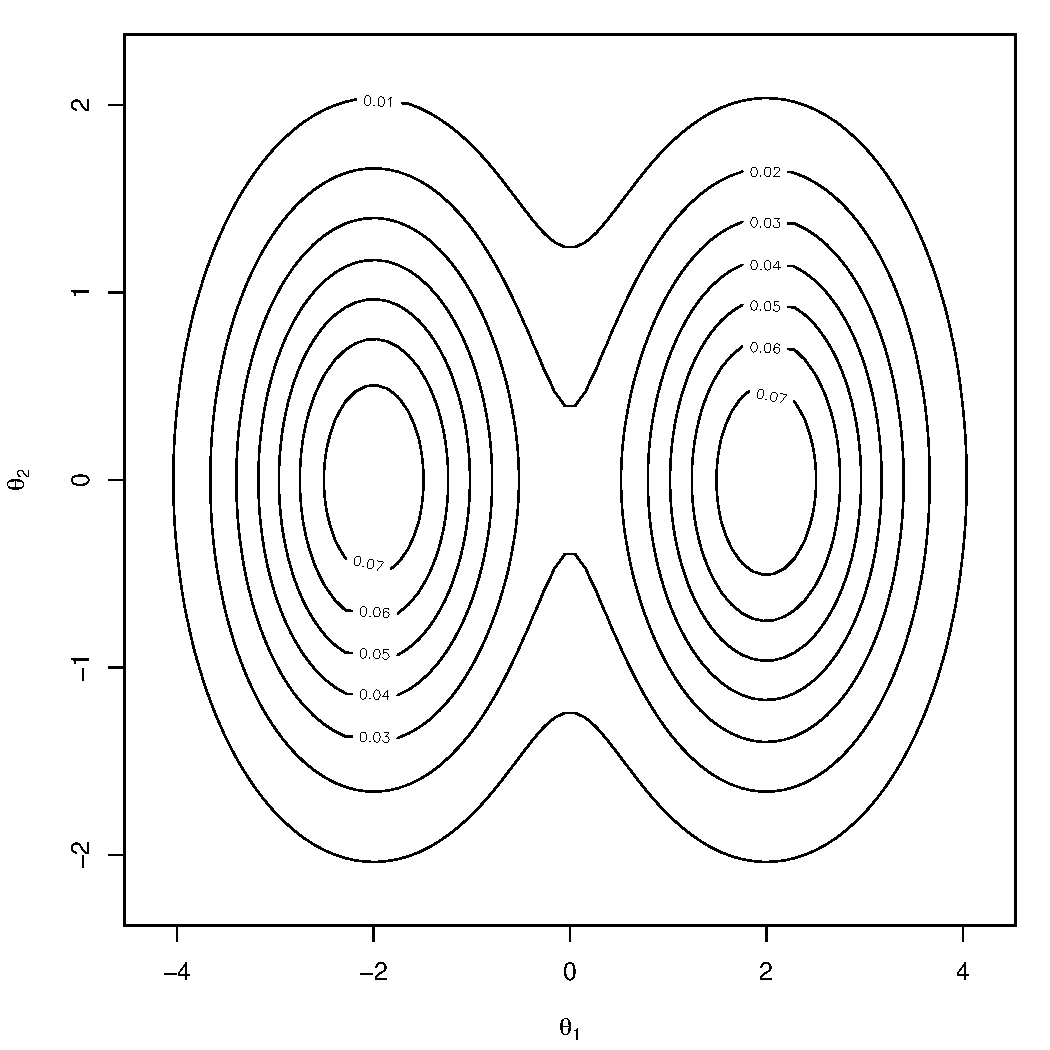
\includegraphics[height=4.9cm,angle=0]{plots/hamiltonianmixture.pdf}
\end{minipage}
\end{tabular}
\end{center}
}






\frame{
\sffamily
\frametitle{Tuning}
\begin{itemize}
\item Hamiltonian Monte Carlo algorithms are not totally automatic, as you still need to decide the size and number of steps, as well as (at least) the covariance matrix associated with the momentum variables.

\vspace{3mm}

\item As with RWMH, tuning HMC algorithms usually requires pilot runs for different values of $\epsilon$ and $L$.  Be careful, optimal values might be different before and after convergence!

\item The value of $\epsilon L$ roughly controls how far you move from the current point.  However, a large value of $\epsilon L$ does not necessarily lead to longer-distance moves (recall the graphs for the Hamiltonian trajectories in $(\bftheta, \bfphi)$).

\item Indeed, the chain produced by a Hamiltonian algorithm could potentially be periodic, but that is rarely the case in practice.  %One solution is to use randomly chosen $\epsilon$ and $L$ (from a relatively narrow range) at each iteration.
\end{itemize}
}






\frame{
\sffamily
\frametitle{Tuning}
\begin{itemize}
\item Assuming that $\epsilon L$ is kept roughly constant, the smaller $\epsilon$ is, the closest the discretized trajectory is to the continuous time one, but more computations are required.

\item The rejection rate of the algorithm is controlled mainly by $\epsilon$ (i.e., how good the discrete-time approximation is).  Values of $\epsilon$ that are too big might lead to unstable trajectories and very low acceptance rates, and the problem might not be obvious in pilot runs because the rejection rate might be very different in different regions of the space.

\item As a rule of thump, the optimal acceptance rate for HMC is around 65\% for high-dimensional problems (against the $\sim$ 23\% for high-dimensional RWMH).
\end{itemize}
}




\frame{
\sffamily
\frametitle{Tuning}
\begin{itemize}
\item If an estimate of $\Var(\bftheta \mid \bfy)$ is available, applying a linear transformation for the position variables so that they have (approximately) variance 1 and no correlation and using independent standard Gaussian momentum variables leads to good performance with a small number of steps 

\item Note that under Gaussian momentum, performance of the algorithm is invariant to linear transformations $\mathbf{B} \theta$ if the momentum variables are multiplied by $\left( \mathbf{B}' \right)^{-1}$.  Hence, alternatively we leave the positions untransformed and use correlated Gaussian momentum variables.

\item In any case, it is a good idea to use different scales for the each momentum variable if the position variables have very different variances.
\end{itemize}
}


\frame{
\sffamily
\frametitle{Implementation}

\begin{itemize}

\item Tuning HMC algorithms can be tricky, but the Stan software was developed for just this purpose. Stan uses its own language for specifying the statistical model.

\item \texttt{hmc-cox.R} provides a Stan implementation for a Cox survival analysis model. See Appendix for more details on Stan and the Cox example.

\item NIMBLE doesn't provide HMC because we're just now implementing automatic differentation and because it's Stan's sweet spot.  
\end{itemize}

}


\frame{
\sffamily
\frametitle{Special cases and extensions}
\begin{itemize}
\item A single step HMC (i.e., $L=1$ ) corresponds to a pre-conditioned Langevin diffusion as used in a Metropolis-Adjusted Langevin Algorithm (MALA).

\item Note that HMC cannot deal with discrete parameters (but see new work from David Dunson's group).

\item HMC can be seen as just another MH kernel, so it can be used for subsets of parameters and combined with other kernels (gives you a way to separate discrete parameters).

\item A number of useful extensions, examples include
\begin{itemize}
\item Riemmanian HMC (non-constant $\mathbf{M}$).
\item ``Splitting'' the Hamiltonian
\item Partial momentum refreshment.
\end{itemize}
\end{itemize}
}




\section{Model selection}

\frame{
\sffamily
\frametitle{Model selection and hypothesis testing}
\begin{itemize}
\item Most of the discussion so far has focused on Monte Carlo methods for point and interval estimation.

\item We move now to discuss MCMC methods in the context of model selection and hypothesis testing.

\item The approach we will focus on turns the model selection problem into an estimation problem for a discrete random variable (the model indicator).
\end{itemize}
}


\frame{
\sffamily
\frametitle{Variable selection}
\begin{itemize}
\item {\bf Example (variable selection in linear models):}  Consider a linear model of the form $\bfy = \bfX \bftheta + \bfepsilon$ with $\bfepsilon \sim \normal( \mathbf{0}, \sigma^2 \mathbf{I} )$, $\mbox{dim} \{ \bfy \} = n$, and $\mbox{dim} \{ \bftheta \} = p$.  We are interested in selecting a subset of the columns of $\bfX$ that explain the response $\bfy$.  

\vspace{1mm}

Hence, since we have a total of $p$ variables, we need to select among $2^p$ models.  Each of these models can be represented using a vector $\bfgamma = (\gamma_1, \ldots, \gamma_p)$ where $\gamma_k = 1$ if variable $k$ is in the model, and $\gamma_k = 0$ otherwise.

\vspace{1mm}

To address this problem from a Bayesian perspective we need to compute the probability associated with each model.  To do so we need a prior distribution $p(\bftheta, \sigma^2, \bfgamma)$ which we will conveniently breakdown as $p(\bftheta \mid \sigma^2,  \bfgamma)  p(\sigma^2 \mid \bfgamma) p( \bfgamma)$.
\end{itemize}
}





\frame{
\sffamily
\frametitle{Variable selection}
\begin{itemize}
\item {\bf Example (variable selection in linear models, cont):}  For the regression coefficients, we focus on priors of the form 
$$
\bftheta \mid \sigma^2 , \bfgamma \sim \normal \left(\bftheta_{\bfgamma} \mid \mathbf{0}, c \sigma^2 
\left\{ \bfX_{\bfgamma}^{T}\bfX_{\bfgamma} \right\}^{-1} \right) \prod_{k : \gamma_k = 0} \delta_{0}(\theta_k)  ,
$$
$\bfX_{\bfgamma}$ denotes the matrix composed of the columns of $\bfX$ for which the associated  $\gamma_k = 1$, and $\delta_0(\cdot)$ denotes the degenerate measure at $0$.

For the variance we have $\sigma^2 \mid \bfgamma \sim \IGam(a,b)$ (which is independent of $\bfgamma)$.

Set $p(\bfgamma) = \frac{\Gamma(1 + \sum_{k=1}^{p} \gamma_i) \Gamma(1 + p - \sum_{k=1}^{p} \gamma_i)}{\Gamma(p + 2)}$, (Beta-Bernoulli prior).

Set $c = n$ (more generally, a prior centered on $n$.)
\end{itemize}
}




\frame{
\sffamily
\frametitle{Variable selection}
\begin{itemize}
\item {\bf Example (variable selection in linear models, cont):}  Note that in this analysis we are really interested in the marginal posterior $p(\bfgamma \mid \bfy)$, and we can think of $\bftheta$ and $\sigma^2$ as ``nuisance'' parameters. Integrating them out we have

{\scriptsize
\begin{multline*}
p(\bfy \mid \bfgamma) = \left(\frac{1}{2\pi}\right)^{\frac{n}{2}} \left|
\mathbf{I} + c\bfX_{\bfgamma} \left(\bfX_{\bfgamma}^{T} \bfX_{\bfgamma}\right)^{-1} \bfX_{\bfgamma}^T \right|^{-\frac{1}{2}} \\
%  
\frac{b^a}{\Gamma(a)}
\frac{\Gamma \left( a + \frac{n}{2} \right)}
{\left( b + \frac{\bfy^T \left\{ \mathbf{I} + c\bfX_{\bfgamma} \left(\bfX_{\bfgamma}^{T} \bfX_{\bfgamma}\right)^{-1} \bfX_{\bfgamma}^T \right\}^{-1}\bfy}{2} \right)^{a + \frac{n}{2}}}  ,
\end{multline*}
}
and the posterior distribution is simply
$$
p(\bfgamma \mid \bfy) = \frac{p(\bfy \mid \bfgamma)p(\bfgamma)}{\sum_{\bfgamma'}p(\bfy \mid \bfgamma')p(\bfgamma')} .
$$

\end{itemize}
}



\frame{
\sffamily
\frametitle{Variable selection}
\begin{itemize}
\item {\bf Example (variable selection in linear models, cont):}  Because $\bfgamma$ can only take a finite number of values, getting these posterior probabilities should be straightforward:
\begin{itemize}
\item This is true when $p$ is relatively small (say $p \le 20$).  In that case the number of models is manageable (with $p=20$ we have 1,048,576 models), and we can actually compute (and store) the probabilities for each model with the resources available in regular computers.

\item However, when $p$ is large we cannot do that anymore (roughly, every 10 extra variables you add multiplies the number of models by 1,000, so you can easily run out of atoms in the universe in a typical problem in genetics ...) 
\end{itemize}

\vspace{1mm}

Hence, even in discrete problems with an ``analytical'' solutions you might want to use simulations to make the problem more manageable.

\end{itemize}
}


\frame{
\sffamily
\frametitle{Variable selection: A Metropolis-Hastings algorithm}
\begin{itemize}
\item {\bf Example (variable selection in linear models, cont):  } A couple of options for constructing a Metropolis-Hasting algorithm:
\begin{itemize}
\item A simple random walk proposal can be constructed by choosing one entry $\gamma_k$ of $\bfgamma$ uniformly at random and generating a new model by setting 
$$
\bfvartheta = (\gamma_1, \ldots, \gamma_{k-1}, 1 - \gamma_k, \gamma_{k+1}, \ldots, \gamma_{p})
$$
\item An independent proposal could be constructed by generating a new model by randomly sampling from a uniform distribution over the entire model, i.e., by letting $\vartheta_k \sim \Ber(1/2)$ independently for each $k$.
\end{itemize}

The acceptance probability in both cases is
$$
\rho(\bfvartheta, \bfgamma) = \min \left\{ 1, \frac{p(\bfvartheta \mid \bfy)}{p(\bfgamma \mid \bfy)} \right\} .
$$
\end{itemize}
}


\frame{
\sffamily
\frametitle{Variable selection}

\begin{itemize}
\item {\bf Example (variable selection in a GLMM):} \cite{gelman2007data} analyzes a dataset of support provided by unmarried fathers to their children's mothers.  The model features are:
\begin{itemize}
\item observations of binary outcomes for each mother/father pair of informal support to the mother
\item observations grouped within 20 cities (with random effects to account for correlation)
\item individual-level predictors
\item city-level predictors including the intensity of child support enforcement by the city
\end{itemize}

\textbf{Scientific question:}  does enforcement by the city impact whether support is provided?


\textbf{Model:}  probit regression with variable selection. 
\end{itemize}
}




\frame{
\sffamily
\frametitle{Reversible Jump}
\begin{itemize}
\item In the case of the linear model we could integrate out the regression coefficients and work exclusively with the vector $\bfgamma$.  Hence, although the size of $\bftheta$ changes with $\bfgamma$, we did not really have to deal with the varying dimension.

\item In the case of the generalized linear model, it is not obvious how we can integrate out the coefficients explicitly.  Hence, our algorithm needs to deal with the fact that the number of coefficients can change. 

\item A slight generalization of Metropolis Hastings algorithms called reversible jump MCMC \citep{Gr95,brooks2003efficient} can be used in this context.
\end{itemize}
}




\frame{
\sffamily
\frametitle{Reversible Jump}
\begin{itemize}
\item Let's start by establishing some notation.
\begin{itemize}
\item Let $K$ index the model of interest.  Associate with such model a prior $p(K)$.

\item Each model $\mathcal{M}_K$ has a set of distinct set of parameters $\bftheta_K$.  The associated prior is $p(\bftheta_K \mid K)$ which depends (explicitly or implicitly) on the dimension $K$.

\item Given model $\mathcal{M}_K$ and parameters $\bftheta_K$, data is generated according to a likelihood $p(\bfy \mid K, \bftheta_K)$.

\item We denote the corresponding posterior distribution as $p(K, \bftheta_K \mid \bfy)$ which can be factorized as 
$$
p(K, \bftheta_K \mid \bfy) = p(K \mid \bfy) p(\bftheta_K \mid K, \bfy)
$$
\end{itemize}
\item Hence, if we could compute $p(K \mid \bfy)$ for all $K$, then model selection would be straightforward.  However, this involves integrating over all other parameters of model!
\end{itemize}
}




\frame{
\sffamily
\frametitle{Reversible Jump}
\begin{itemize}
\item To derive the algorithm:
\begin{itemize}
\item First, augment each vector $\bftheta_K$ with auxiliary variables $\bfu_K$, so that the dimension of $(\bftheta_K, \bfu_K)$ \textit{is the same} for all $K$.
\item Second, define a (consistent) collection of deterministic transformations $T_{K,K'} \left\{ (\bftheta_K, \bfu_K), (\bftheta_{K'}, \bfu_{K'}) \right\}$ that map the augmented parameter spaces of different models (this is typically done by defining transformation only between ``neighboring'' models).
\end{itemize}

\item Note that, in some sense, the proposals are \textit{deterministic} because the transformation is deterministic.  (However, the presence of the auxiliary variables $\bfu_K$ introduces randomness).
\end{itemize}
}





\frame{
\sffamily
\frametitle{Reversible Jump}
\begin{itemize}

\item The acceptance probability becomes
\begin{multline*}
\left\{ 1 ,
\frac{p\left(K^{(p)}, \theta^{(p)}_{K^{(p)}} \mid \bfy \right)  }{p\left(K^{(c)}, \theta^{(c)}_{K^{(c)}} \mid \bfy \right)}
%
\frac{g_{K^{(p)}} \left( \bfu^{(p)}_{K^{(p)}} \right)}{g_{K^{(c)}} \left( \bfu^{(c)}_{K^{(c)}} \right)}
%
\frac{d_{K^{(p)}, K^{(c)}}}{d_{K^{(c)}, K^{(p)}}} \right.  \\  \left.
%
\left|  \frac{\partial T_{K^{(c)}, K^{(p)}} \left( \bftheta^{(c)}_{K^{(c)}}, \bfu^{K^{(c)}}_{(c)} \right) }
{ \partial \left( \bftheta^{(c)}_{K^{(c)}}, \bfu^{K^{(c)}}_{(c)} \right)  } \right|
 \right\}
\end{multline*}
where $g_K(\bfu_K)$ is the density of the auxiliary variables and $d_{K, K'}$ is the probability of proposing a move to state $K'$ when you are currently in state $K$.

\item Note that the auxiliary variables $\bfu_K$ do not need to be stored and can be simulated on the fly ...
\end{itemize}
}





\frame{
\sffamily
\frametitle{Reversible Jump}
\begin{itemize}
\item With these preliminaries, and assuming the current state of your chain is $\left( K^{(c)}, \bftheta_{K^{(c)}}^{(c)} \right)$ the RJMCMC algorithm is:
\begin{enumerate}
\item Propose a move to model $\mathcal{M}_{K^{(p)}}$ with probability $d_{K^{(c)}, K^{(p)}}$.
\item Generate $\bfu^{(p)} \sim g_{K^{(p)}}$ and $\bfu^{(c)} \sim g_{K^{(c)}}$.
\item Set $\left( \bftheta^{(p)}_{K^{(p)}},  \bfu^{(p)}_{K^{(p)}} \right) = T_{K^{(c)}, K^{(p)}}\left( \bftheta^{(c)}_{K^{(c)}},  \bfu^{(c)}_{K^{(c)}} \right)$.
\item Accept this proposal with probability
{\scriptsize \begin{multline*}
\left\{ 1 ,
\frac{p\left(K^{(p)}, \theta^{(p)}_{K^{(p)}} \mid \bfy \right)  }{p\left(K^{(c)}, \theta^{(c)}_{K^{(c)}} \mid \bfy \right)}
%
\frac{g_{K^{(p)}} \left( \bfu^{(p)}_{K^{(p)}} \right)}{g_{K^{(c)}} \left( \bfu^{(c)}_{K^{(c)}} \right)}
%
\frac{d_{K^{(p)}, K^{(c)}}}{d_{K^{(c)}, K^{(p)}}} \right.  \\  \left.
%
\left|  \frac{\partial T_{K^{(c)}, K^{(p)}} \left( \bftheta^{(c)}_{K^{(c)}}, \bfu^{K^{(c)}}_{(c)} \right) }
{ \partial \left( \bftheta^{(c)}_{K^{(c)}}, \bfu^{K^{(c)}}_{(c)} \right)  } \right|
 \right\}
\end{multline*}}
\end{enumerate}
\end{itemize}
}



\frame{
\sffamily
\frametitle{Reversible Jump}
\begin{itemize}
\item The deterministic move can be justified as the limit of random proposals whose variability goes to zero.

\item Remember that the proposals need to be reversible!

\item Note that there are potentially a number of simplifications in the previous acceptance probability.  For example, you typically do not need to generate all the entries of $\bfu^{(c)}_{K^{(c)}}$ and $\bfu^{(p)}_{K^{(p)}}$.

\item Note that the auxiliary variable densities determine the proposed values in for model $K^(p)$ so need to be chosen carefully - comparable to independent M-H schemes.

\item The transitions above need to be combined with ``regular'' transition kernels within each dimension!
\end{itemize}
}





\frame{
\sffamily
\frametitle{Reversible Jump}

\begin{itemize}
{\small
\item {\bf Example (variable selection in a GLMM): } Reversible jump here is quite simple. At each iteration propose to add or remove the variable depending on whether it is currently in the model.

The deterministic transformation between the full and reduced models is $ T_{0,1}{(\theta,u)} = (\theta, \beta_e)$, so $\beta_e^{(p)} = u^{(c)}$, where $\theta$ are the parameters always in the model, $\beta_e$ is the enforcement coefficient, and $u$ is the single auxiliary variable. 

$d_{0,1} = d_{1,0} = 1$ and the Jacobian is one, so the proposals involve:

\begin{itemize}
\item Addition: propose $\beta_e^{(p)} = u^{(c)}$ from $u^{(c)} \sim g_0(u)$ with term $1/g_0(u^{(c)})$ in the acceptance ratio
\item Removal:  propose removal ($u^{(p)}=\beta_e^{(c)}$)  with term $g_0(\beta_e^{(c)})$ in the acceptance ratio
\end{itemize}

Note that auxiliary variable density $g_0(u)$ plays the role of a constant proposal distribution for $\beta_e$ so should be well-chosen.

See \texttt{rjmcmc-childSupport.R} for the implementation using a user-defined sampler in NIMBLE.
}
\end{itemize}
}











\section{SMC}

\frame{
\sffamily
\frametitle{Importance sampling}
\begin{itemize}
\item Let's go back to the problem of approximating integrals of the form
$$
\int h(\bftheta) p(\bftheta \mid \bfy) \dd \bftheta  ,
$$
where $h$ is an integrable function and $p(\bftheta \mid \bfy)$ is the posterior distribution induced by our model.

\item We return to the idea of ``replacing'' $p(\bftheta \mid \bfy)$ with $g(\bftheta)$ from which it is easy to generate, we can write
\begin{align*}
\int h(\bftheta) p(\bftheta \mid \bfy) \dd \bftheta  &= \int h(\bftheta) \frac{ p(\bftheta \mid \bfy)}{g(\bftheta)} g(\bftheta) \dd \bftheta  \\ 
&= \int h(\bftheta) w(\bftheta, \bfy) g(\bftheta) \dd \bftheta ,
\end{align*}
where $w(\bftheta, \bfy) = \frac{ p(\bftheta \mid \bfy)}{g(\bftheta)}$ is a ``weight'' function.
\end{itemize}
}




\frame{
\sffamily
\frametitle{Importance sampling}
\begin{itemize}
\item As long as the support of $g$ contains the support of $p(\bftheta \mid \bfy)$, the WLLN ensures that if $\bftheta_1^{(1)}, \ldots, \bftheta_1^{(B)}$ are independent and identically distributed samples from $g$ then
\begin{align*}
\frac{\sum_{b=1}^{B} h\left( \bftheta^{(b)} \right) w\left( \bftheta^{(b)} , \bfy \right) }
{\sum_{b=1}^{B}  w\left( \bftheta^{(b)} , \bfy \right) }  & \underset{B \to \infty}{\longrightarrow} \E \left\{ h\left( \bftheta^{(b)} \right) \right\} 
\end{align*}

\item Almost any $g$ works in principle.  However, if you want your estimator to have a finite variance, then  you need $g$ such that
$$
\int h^2(\bftheta) \frac{p^2(\bftheta \mid \bfy)}{g(\bftheta)} \dd \bftheta  < \infty .
$$
A necessary condition for this to be satisfied is that $g$ has heavier tails than $p(\bftheta \mid y)$!
\end{itemize}
}







\frame{
\sffamily
\frametitle{Importance sampling}
\begin{itemize}

\item The optimal importance sampling distribution should be a good approximation to 
$h(\bftheta) p(\bftheta \mid \bfy)$ rather than a good approximation to $p(\bftheta \mid \bfy)$.  For example, consider $p = \Pr(X > 2)$ where $X\sim \Cauchy(0,1)$.

\begin{itemize}
\item  The naive estimator is given by 
$$
\hat{p}_1 = \frac{1}{B} \sum_{b=1}^{B} \ind_{\{ x^{(b)} > 2 \}} ,
$$
where $x^{(b)} \sim \Cauchy(0,1)$.  Its variance $0.127/B$.

\item A much better alternative is to estimate $p$ using 
$$
\hat{p}_2 = \frac{1}{B} \sum_{b=1}^{B} \frac{ \left( x^{(b)} \right)^{-2} }{2\pi \left\{ 1 + \left( x^{(b)} \right)^{-2} \right\}} ,
$$
where $x^{(b)} \sim \Uni[0,1/2]$.  Its variance $0.095/B$.
\end{itemize}

\end{itemize}
}




\frame{
\sffamily
\frametitle{Importance sampling}
\begin{itemize}
\item A way to evaluate the efficiency of the algorithm is through the equivalent sample size (ESS):
$$
ESS =   \frac{\left\{ \sum_{b=1}^{B} w\left( \bftheta^{(b)} , \bfy \right) \right\}^2}{\sum_{b=1}^{B} \left\{ w\left( \bftheta^{(b)} , \bfy \right)\right\}^2 }  .
$$
The interpretation of this ESS is analogous to that of the ESS we discussed for MCMC methods.  In particular, if all the weights are identical then $ESS = B$, while if all weight is concentrated on a single particle then $ESS = 1$.
\end{itemize}
}




\frame{
\sffamily
\frametitle{Importance sampling}
\begin{itemize}
\item {\bf Example (unknown Gaussian mean with Cauchy priors):  }  Consider a simple model where $y_1, \ldots, y_n$ are iid with $y_i \sim \normal(\theta, 1)$, and where we use a ``robust'' prior $\theta \sim \Cauchy(0,1)$.  The posterior distribution is proportional to
\begin{align*}
\left( \frac{1}{1 + \theta^2} \right) \exp \left\{ -\frac{n}{2} \left(  \theta^2 - 2 \theta \bar{y} \right) \right\}  .
\end{align*}

We are interested in computing the posterior mean: 
\begin{align*}
\E\left\{ \theta \mid \bfy \right\} = \frac{\int_{-\infty}^{\infty} \left( \frac{\theta}{1 + \theta^2} \right) \exp \left\{ -\frac{n}{2} \left(  \theta^2 - 2 \theta \bar{y} \right)  \right\}  \dd \theta
}
%
{ \int_{-\infty}^{\infty} \left( \frac{1}{1 + \theta^2} \right) \exp \left\{ -\frac{n}{2} \left(  \theta^2 - 2 \theta \bar{y} \right)  \right\}  \dd \theta}.
\end{align*}
An analytic solution for this expectation is not available.
\end{itemize}
}




\frame{
\sffamily
\frametitle{Importance sampling}
\begin{itemize}
\item {\bf Example (unknown Gaussian mean with Cauchy priors):  }  You could use the prior as the importance distribution:
$$
\E\left\{ \theta \mid \bfy \right\} \approx \frac
{\sum_{b=1}^{B} \theta^{(b)} \exp \left\{ -\frac{n}{2} \left(  \theta^{(b)2} - 2 \theta^{(b)} \bar{y} \right)  \right\}  }
{\sum_{b=1}^{B} \exp \left\{ -\frac{n}{2} \left(  \theta^{(b)2} - 2 \theta^{(b)} \bar{y} \right)  \right\}  }.
$$
This estimator is implemented in \texttt{impsampex\_v1.R}.  
%Note that just a few samples (located around the mean of the data) receive most of the weight!  Accordingly, the ESS is very small (around 4). Hence, this estimator has a very large variance (run the algorithm multiple times to get a sense of the Monte Carlo error).

A more reasonable importance function use knowledge about the shape of $p(\theta \mid \bfy)$
{\scriptsize $$
\E\left\{ \theta \mid \bfy \right\} \approx \frac
{\sum_{b=1}^{B} \theta^{(b)}  \left( \frac{1 +  n\{\theta^{(b)} - \bar{y}\}^2}{1 + \theta^{2(b)}} \right) \exp \left\{ -\frac{n}{2} \left(  \theta^{(b)2} - 2 \theta^{(b)} \bar{y} \right)  \right\}  }
{\sum_{b=1}^{B} \left( \frac{1 +  n\{\theta^{(b)} - \bar{y}\}^2}{1 + \theta^{2(b)}} \right) \exp \left\{ -\frac{n}{2} \left(  \theta^{(b)2} - 2 \theta^{(b)} \bar{y} \right)  \right\}  }.
$$ }
where $\theta^{(b)} \sim \Cauchy(\bar{y}, 1/n)$.  See \texttt{impsampex\_v2.R}.

\end{itemize}
}








\frame{
\sffamily
\frametitle{Importance sampling}
\begin{itemize}
\item Importance sampling schemes can also be interpreted as providing an approximation to $p(\bftheta \mid \bfy)$:
$$
\hat{p}_{B}(\bftheta \mid \bfy) =  \sum_{b=1}^{B}  \omega \left(\bftheta^{(b)}, \bfy \right) \delta_{\bftheta^{(b)}} (\bftheta)  ,
$$
where $\delta_x (\bftheta)$ denotes the Dirac point mass at $x$.

\item Then, a fancy way to write the importance sampling estimator is as
$$
\int h(\bftheta) \hat{p}_B(\bftheta \mid y) \dd \bftheta \to \int h(\bftheta) p_B(\bftheta \mid y) \dd \bftheta  .
$$
Since this is true for any integrable function $h$, it implies that
\begin{align*}
 \hat{p}_B(\bftheta \mid y)  &\to p_B(\bftheta \mid y)   & \mbox{ in distribution}  .
\end{align*}
\end{itemize}
}







\frame{
\sffamily
\frametitle{Sequential Importance Sampling}
\begin{itemize}
\item When $\bftheta$ is high dimensional, constructing a good instrumental distribution can be very hard.  

\item One option is to construct it in pieces by (for example) writing
\begin{multline*}
g(\bftheta \mid \bfy) = g(\theta_T \mid \theta_{T-1}, \theta_{T-2}, \ldots, \theta_{1}, \bfy) \\
%
g(\theta_{T-1} \mid \theta_{T-2}, \ldots, \theta_{1}, \bfy) \cdots  g(\theta_{2} \mid \theta_{1}, \bfy) g(\theta_1\mid \bfy)
\end{multline*}

\item Particularly useful for models of the form:
$$
p(\bftheta_{1:T} \mid \bfy_{1:T}) \propto \prod_{t=1}^{T} p\left(\bfy_t \mid \bfy_{1:(t-1)} , \bftheta_{1:t} \right)
%
p\left(\bftheta_t \mid \bftheta_{1:(t-1)}  \right)
$$
where $\bfy_{1:t} = (\bfy_1, \ldots, \bfy_{t})$ and $\bftheta_{1:t} = (\bftheta_1, \ldots, \bftheta_{t})$.The key is that $p\left(\bfy_t \mid \bfy_{1:(t-1)} , \bftheta_{1:t} \right)$ does not depend on $\bftheta_{(t+1):T}$.
\end{itemize}
}




\frame{
\sffamily
\frametitle{Sequential Importance Sampling}
\begin{itemize}
\item The SIS algorithm proceeds by repeating the following steps for $t=1,\ldots,T$:
\begin{itemize}
\item Given a representation $\hat{p}\left(\bftheta_{1:t} \mid \bfy_{1:t}\right) = \sum_{b=1}^{B}\omega^{(b)}_{t} \delta_{\hat{\bftheta}_{1:t}^{(b)}}$ 
\begin{enumerate}
\item For $b=1, \ldots, B$ sample $\hat{\bftheta}_{t+1}^{(b)} \sim g\left(\bftheta^{(b)}_{t+1} \mid \bftheta_{1:t} , \bfy \right)$ and let $\hat{\bftheta}_{1:(t+1)}^{(b)} = \left(\hat{\bftheta}_{1:t}^{(b)}, \hat{\bftheta}_{t+1}^{(b)} \right)$.

\item Construct $\hat{p}\left(\bftheta_{1:(t+1)} \mid \bfy_{1:(t+1)}\right) = \sum_{b=1}^{B} \omega^{(b)}_{t+1} \delta_{\hat{\bftheta}_{1:(t+1)}^{(b)}}$ where 
$$
\omega_{t+1}^{(b)}  \propto \omega_{t}^{(b)} \frac{p\left(\bfy_{1:(t+1)} \mid \bfy_{1:t}, \hat{\bftheta}^{(b)}_{1:(t+1)} \right) p\left(\hat{\bftheta}^{(b)}_{t+1} \mid \hat{\bftheta}^{(b)}_{1:t} \right)}{g\left(\hat{\bftheta}^{(b)}_{t+1} \mid \hat{\bftheta}^{(b)}_{1:t} \bfy \right)}  .
$$
\end{enumerate}
\end{itemize}

\item Note that the end of this process we have a particle representation for $p(\bftheta_{1:T} \mid \bfy_{1:T})$ (the joint posterior).
\end{itemize}
}





\frame{
\sffamily
\frametitle{Sequential Importance Sampling}
\begin{itemize}
\item The main issue with SIS is degeneracy.  As the algorithm proceeds, a single particle tends to receive all the weight $\Rightarrow$ ESS tends to be very small.

\item This is true even if the instrumental distributions are chosen optimally (which is very rarely the case!)

\item Hence, for large $T$, estimates derived from the algorithm can have enormous variances.

\item Although degeneracy is an issue with every sequential Monte Carlo scheme, but it can often be alleviated by focusing on $p(\bftheta_t \mid \bfy_{1:t})$ (the marginal for the parameters at time $t$) rather than $p(\bftheta_{1:t} \mid \bfy_{1:t})$.
\end{itemize}
}






\frame{
\sffamily
\frametitle{State-space models}
\begin{itemize}
\item State space models, which are particularly amenable to computation using variations of importance sample, are defined recursively through an \textit{observational equation}
\begin{align*}
\bfy_{t} \mid \bftheta_{t} &\sim p(\bfy_{t} \mid \bftheta_{t})  ,    &   t=1,\ldots,T,
\end{align*}
and an \textit{evolution equation}
\begin{align*}
\bftheta_{t} \mid \bftheta_{t-1} &\sim p(\bftheta_{t} \mid \bftheta_{t-1})  ,    &   t=1,\ldots,T,
\end{align*}
(together with an \textit{initial distribution} $\bftheta_{0} \sim p(\bftheta_{0})$).

\item We typically interpret the index $t$ as representing ``time'', but it could represent other things (e.g., position in the genome).

\item State-space models include a number of well known models (hidden Markov models, dynamic linear models, ARMA models, etc.)
\end{itemize}
}







\frame{
\sffamily
\frametitle{State-space models}
\begin{itemize}
\item With state-space models there is typically two types of tasks that we are interested in carrying out:
\begin{itemize}
\item Computing the posterior distribution $p(\bftheta_{t} \mid \bfy_{1:t})$ for each $t=1, \ldots, T$.  Typically we want to do this by somehow ``updating'' $p(\bftheta_{t-1} \mid \bfy_{1:(t-1)})$ rather than recomputing from scratch.  We call this process \textit{filtering}.

\item Computing the posterior distribution $p( \bftheta_1 , \ldots, \bftheta_T\mid \bfy_{1:T})$, preferably by reusing information available from the computation of the filtering distributions.  We call this process \textit{smoothing}.
\end{itemize}

\item Note that we usually do not care about $p(\bftheta_{1:t} \mid \bfy_{1:t})$.

\item Also, if we can carry out the filtering step, we can also easily make predictions.
 \end{itemize}
}






\frame{
\sffamily
\frametitle{Filtering:  Sampling Importance Resampling}
\begin{itemize}
\item Given the Markovian definition of state-space models, it is very natural to employ proposal distributions of the form $g(\bftheta_t \mid \bftheta_{t-1}, \bfy_t)$ (i.e., one that depends only on the previous state and the current observation).

\item Furthermore, although using the prior as your instrumental distribution is typically a poor idea, the simplest algorithms further assume that $g(\bftheta_t \mid \bftheta_{t-1}, \bfy_t) = p(\bftheta_t \mid \bftheta_{t-1})$.  This leads to simplifications in the form of the weights

\item Finally, to increase the diversity of the particles, rather than just updating the weights consider adding a resampling step in which a subset of the particle at time $t$ are selected to create the particles at $t+1$.

\item These modifications to SIS lead to the sampling importance resampling (SIR) algorithm.
\end{itemize}
}






\frame{
\sffamily
\frametitle{Filtering:  Sampling Importance Resampling}
\begin{itemize}
\item The SIR algorithm proceeds by repeating the following steps for $t=1,\ldots,T$:
\begin{itemize}
\item Given a particle representation $\hat{p}\left(\bftheta_{t} \mid \bfy_{1:t}\right) = \sum_{b=1}^{B} \omega^{(b)}_{t} \delta_{\hat{\bftheta}_{t}^{(b)}}$ 
\begin{enumerate}
\item For $b=1, \ldots, B$ sample $\tilde{\bftheta}_{t}^{(b)} \sim \hat{p}\left(\bftheta_{t} \mid \bfy_{1:t}\right)$.

\item For $b=1, \ldots, B$ sample $\hat{\bftheta}_{t+1}^{(b)} \mid \tilde{\bftheta}_{t}^{(b)} \sim p\left(\bftheta_{t+1} \mid \tilde{\bftheta}^{(b)}_{t}\right)$.

\item Construct $\hat{p}\left(\bftheta_{t+1} \mid \bfy_{1:(t+1)}\right) = \sum_{b=1}^{B} \omega^{(b)}_{t+1} \delta_{\hat{\bftheta}_{t+1}^{(b)}}$ where 
$$
\omega^{(b)}_{t+1} = \frac{p\left(\bfy_{t+1} \mid \hat{\bftheta}^{(b)}_{t+1}\right)}{\sum_{\ell =1}^{B} p\left(\bfy_{t+1} \mid \hat{\bftheta}^{(\ell)}_{t+1} \right)}  .
$$
\end{enumerate}
\end{itemize}
\item It is very important to note that because of the resampling step in (1) the dependence between $\bftheta_{t}^{(b)}$ and $\bftheta_{t+1}^{(b)}$ is broken and the SIR algorithm only gives you a representation for $p\left(\bftheta_{t+1} \mid \bfy_{1:(t+1)}\right)$ rather than for $p\left(\bftheta_{1:(t+1)} \mid \bfy_{1:(t+1)}\right)$

\end{itemize}
}






\frame{
\sffamily
\frametitle{Filtering:  Sampling Importance Resampling}
\begin{itemize}
\item {\bf Example (a simple linear Gaussian system):}  Consider the linear Gaussian state-space model with
\begin{align*}
y_{t} \mid \theta_{t} &\sim \normal( \theta_{t} , \sigma^2)  ,  &
\theta_{t} \mid \theta_{t-1} &\sim \normal(\theta_{t-1}, \tau^2)  ,  &
\theta_0 &\sim \normal(m_0, C_0^2)  .
\end{align*}

If we assume that $\sigma^2$ and $\tau^2$ are known, then the filtering distributions can be obtained in closed form.  In particular, $\bftheta_t \mid \bfy_{1:t} \sim \normal \left( m_t, C_t^2 \right)$ where
\begin{align*}
m_t &= \frac{\frac{y_t}{\sigma^2} + \frac{m_{t-1}}{\tau^2 + C_{t-1}^2}}{\frac{1}{\sigma^2} + \frac{1}{\tau^2 + C_{t-1}^2}}     ,    &    
%
C_t^2 &= \frac{1}{\frac{1}{\sigma^2} + \frac{1}{\tau^2 + C_{t-1}^2}}  .
\end{align*}

These recursions are known as the Kalman filter in engineering.
\end{itemize}
}





\frame{
\sffamily
\frametitle{Filtering:  Sampling Importance Resampling}
\begin{itemize}
\item {\bf Example (a simple linear Gaussian system, cont):}  The SIR algorithm for this problem takes the form
\vspace{1.5mm}

\begin{enumerate}
\item For $b=1, \ldots, B$ sample $\tilde{\theta}_{t}^{(b)} \sim \hat{p}\left(\theta_{t} \mid \bfy_{1:t}\right)$.

\item For $b=1, \ldots, B$ sample $\hat{\theta}_{t+1}^{(b)} \mid \tilde{\theta}_{t}^{(b)} \sim \normal \left(\theta_{t+1} \mid \tilde{\theta}^{(b)}_{t}, \tau^2 \right)$.

\item Construct $\hat{p}\left(\theta_{t+1} \mid \bfy_{1:(t+1)}\right) = \sum_{b=1}^{B} \omega^{(b)}_{t+1} \delta_{\hat{\theta}_{t+1}^{(b)}}$ where 
$$
\omega^{(b)}_{t+1} = \frac{\normal\left(y_{t+1} \mid \hat{\theta}^{(b)}_{t+1}, \sigma^2\right)}{\sum_{\ell =1}^{B} \normal\left(y_{t+1} \mid \hat{\theta}^{(\ell)}_{t+1} , \sigma^2 \right)} .
$$
\end{enumerate}

\vspace{1mm}  The file \texttt{GaussianSIR.R} implements this SIR algorithm using NIMBLE and compares it against the closed-form solution.
\end{itemize}
}






\frame{
\sffamily
\frametitle{Filtering:  Sampling Importance Resampling}
\begin{itemize}
\item {\bf Example (a simple linear Gaussian system, cont):}  Comparing estimates based on the closed-form recursions and the SIR filter
\end{itemize}
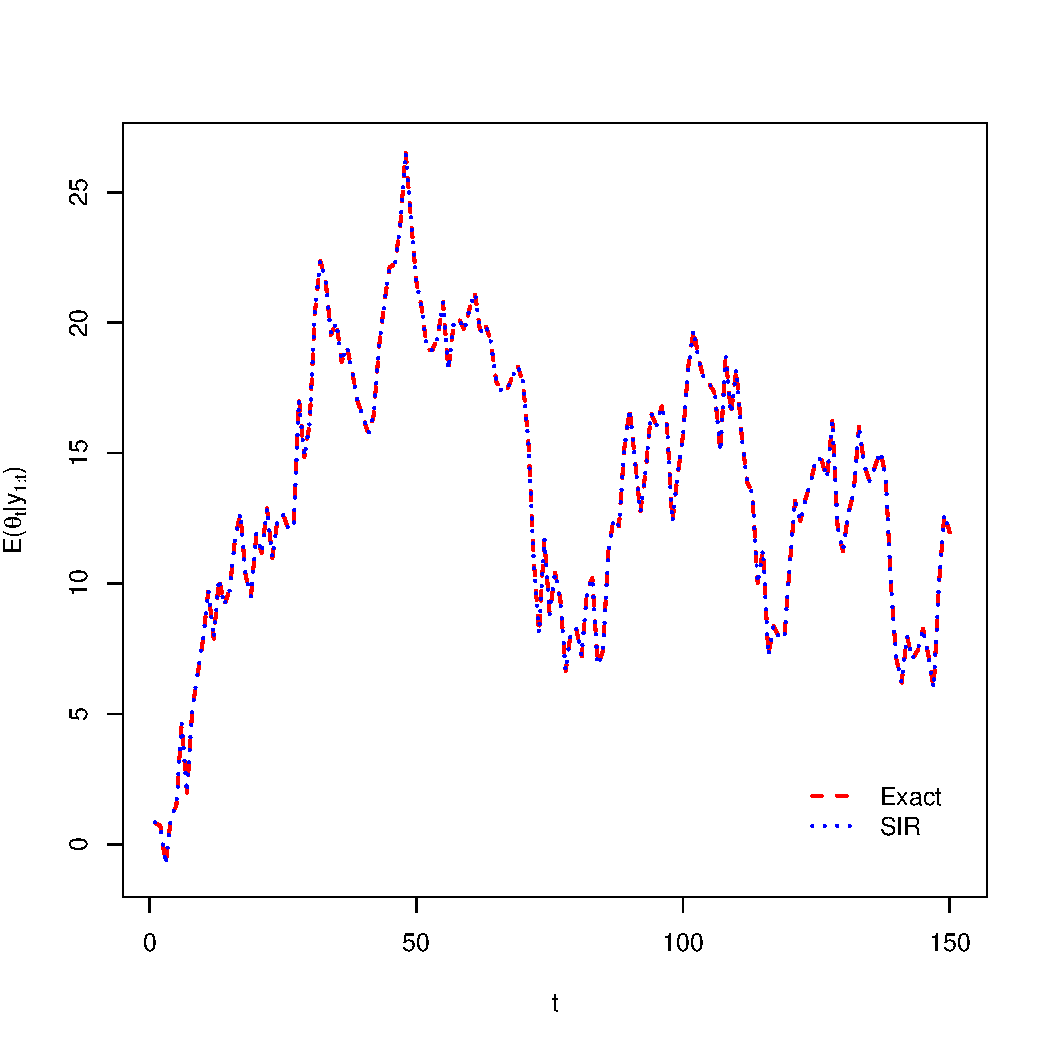
\includegraphics[height=5.6cm,angle=0]{plots/Gaussian_means.pdf}
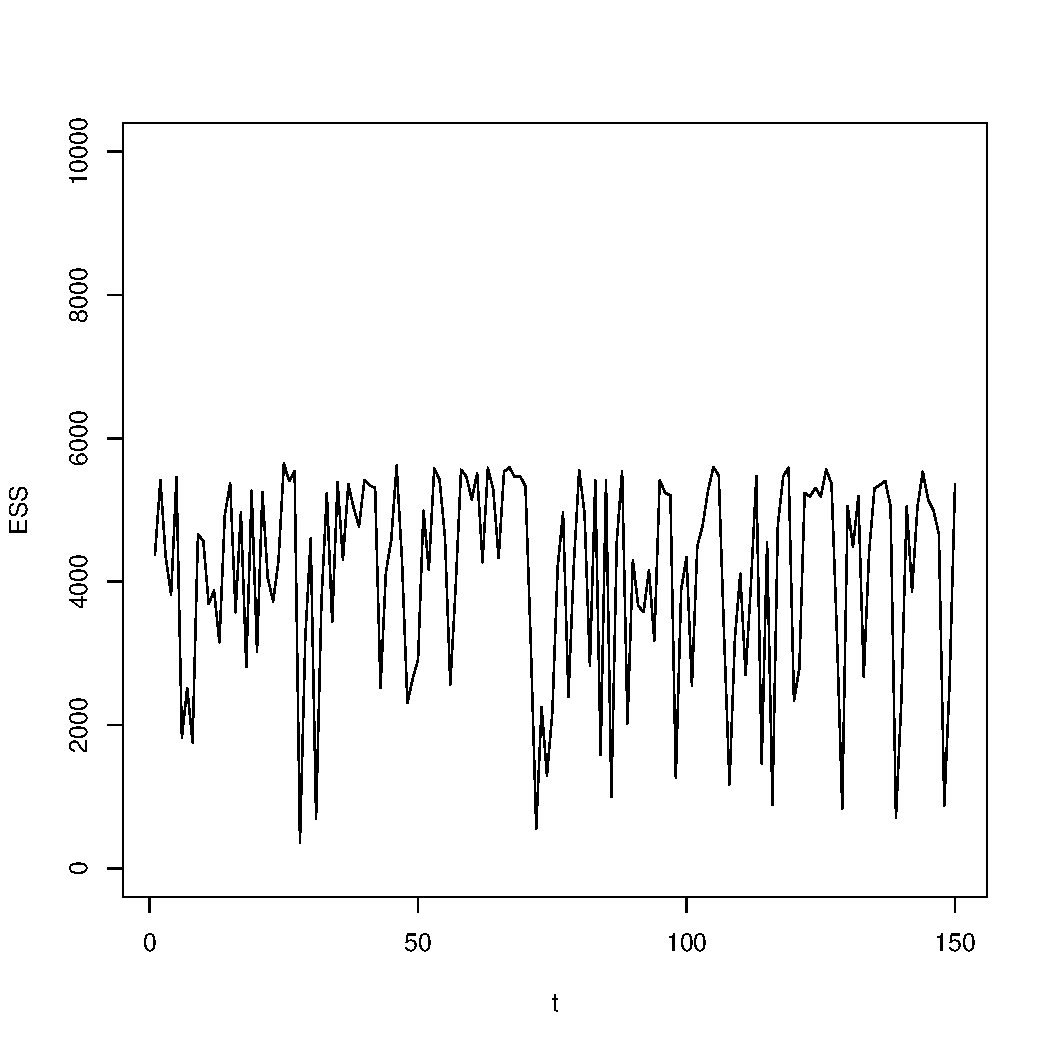
\includegraphics[height=5.6cm,angle=0]{plots/Gaussian_ESSintime.pdf}
}






\frame{
\sffamily
\frametitle{Filtering:  Auxiliary particle filters}
\begin{itemize}
\item APFs reverse the order of resampling and reweighting:
\begin{itemize}
\item Given a particle representation $\hat{p}\left(\bftheta_{t} \mid \bfy_{1:t}\right) = \sum_{b=1}^{B} \omega^{(b)}_{t} \delta_{\hat{\bftheta}_{t}^{(b)}}$ 
\begin{enumerate}

\item For $b=1, \ldots, B$ construct a first-stage weight 
$$
\varpi^{(b)}_{t} = \frac{\omega^{(b)}_{t} p\left(\bfy_{t+1} \mid \bfmu^{(b)}_{t}\right)}{\sum_{\ell =1}^{B} \omega^{(\ell)}_{t} p\left(\bfy_{t+1} \mid \bfmu^{(\ell)}_{t} \right)}  .
$$
where $\bfmu_{t}^{(b)} = \E\left(\bftheta_{t+1} \mid \hat{\bftheta}_{t}^{(b)} \right)$.

\item For $b=1, \ldots, B$ sample $\xi_{t}^{(b)} \sim \sum_{\ell=1}^{B}\varpi^{(\ell)}_{t} \delta_{\ell}$.

\item For $b=1, \ldots, B$ sample $\hat{\bftheta}_{t+1}^{(b)} \mid \hat{\bftheta}_{t}^{(\xi_{t}^{(b)})} \sim p\left(\bftheta_{t+1} \mid \hat{\bftheta}^{(\xi_{t}^{(b)})}_{t}\right)$.

\item Construct $\hat{p}\left(\bftheta_{t+1} \mid \bfy_{1:(t+1)}\right) = \sum_{b=1}^{B} \omega^{(b)}_{t+1} \delta_{\hat{\bftheta}_{t+1}^{(b)}}$ where 
$$
\omega^{(b)}_{t+1} \propto  \frac{p\left(\bfy_{t+1} \mid \hat{\bftheta}^{(\xi_{t}^{(b)})}_{t+1}\right)}{p\left(\bfy_{t+1} \mid \bfmu^{(\xi_{t}^{(b)})}_{t}\right)}   .
$$
\end{enumerate}
\end{itemize}
\end{itemize}
}






\frame{
\sffamily
\frametitle{Filtering:  Auxiliary particle filters}
\begin{itemize}
\item {\bf Example (a simple linear Gaussian system, cont):}  The APF for the linear Gaussian system we described in our previous example (see file \texttt{GaussianAPF.R}) gives a lower average ESS (1687 vs.\ SIR's 4117).
\end{itemize}
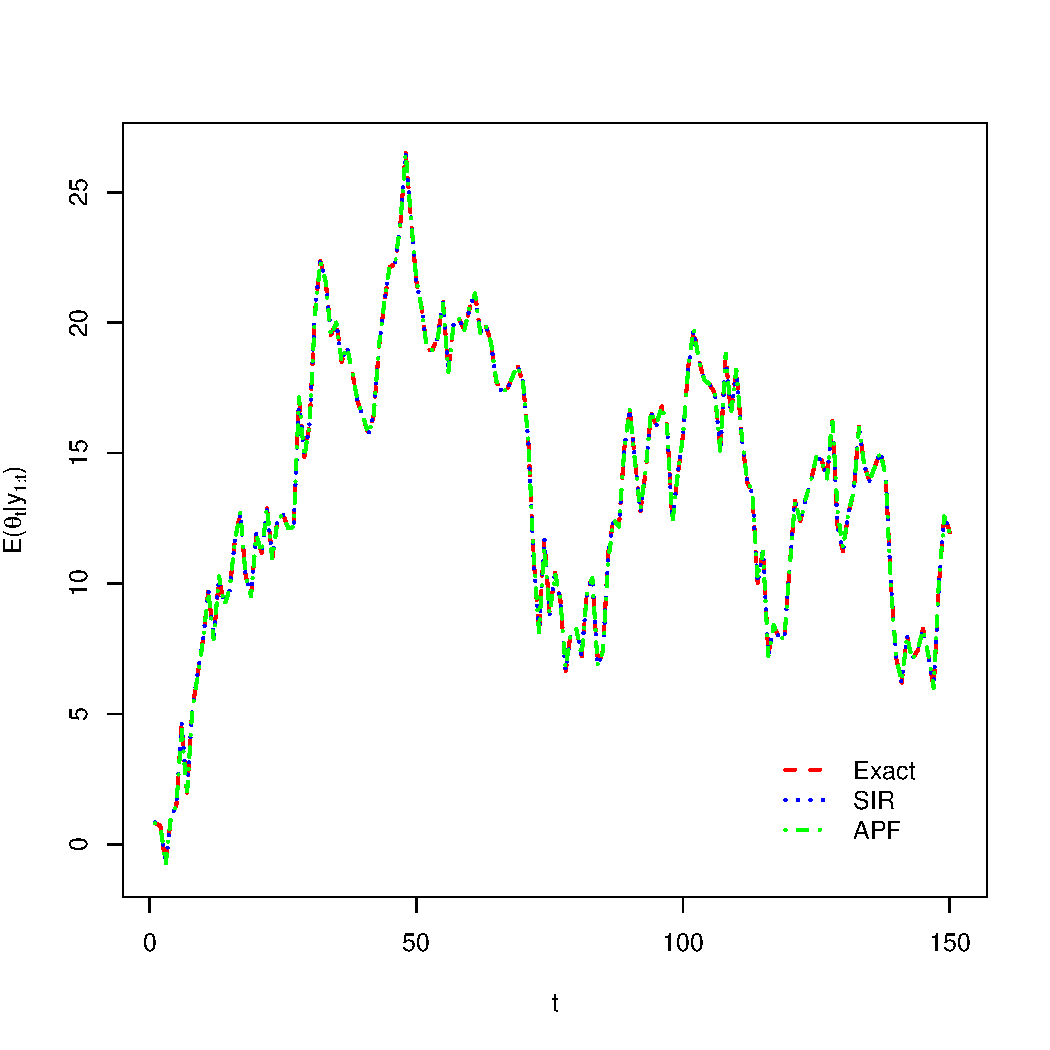
\includegraphics[height=5.6cm,angle=0]{plots/Gaussian_means_APF.pdf}
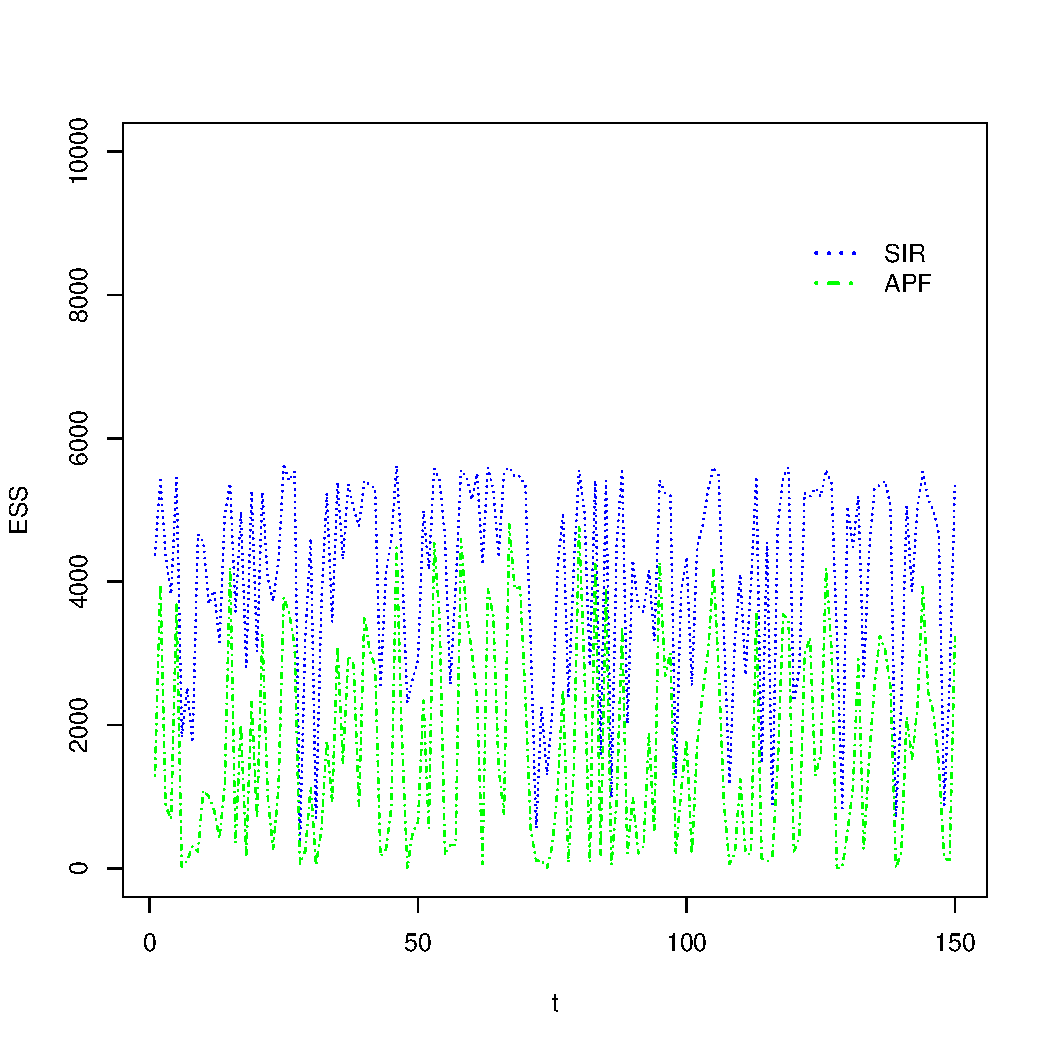
\includegraphics[height=5.6cm,angle=0]{plots/Gaussian_ESSintime_APF.pdf}
}





\frame{
\sffamily
\frametitle{Smoothing}
\begin{itemize}
\item Particle smoothing refers to the process of generating samples from $p(\bftheta_{1:T} \mid \bfy_{1:T})$ using the particles associated with the approximations $\hat{p}(\bftheta_t \mid \bfy_{1:T}) = \sum_{b=1}^{B} \omega_t^{(b)} \delta_{\hat{\bftheta}^{(b)}_{t}}$.

\item The simplest smoothing algorithm was proposed by \cite{godsill2004monte}.  It generates a sample trajectory $\left( \bar{\theta}^{(1)}, \ldots, \bar{\theta}^{(B)} \right)$ through the following steps:

\vspace{1mm}

\begin{enumerate}
\item Sample $\bar{\theta}_{(T)} \sim \hat{p}(\bftheta_T \mid \bfy_{1:T})$.

\vspace{1mm}


\item For $t=T-1, T-2, \ldots, 1$, repeat: 

\begin{enumerate}
\item Calculate $\varpi_{t \mid t+1}^{(b)} \propto \omega_t^{(b)} p\left( \bar{\bftheta}_{t+1} \mid \hat{\bftheta}^{(b)}_{t} \right)$ for each $b=1,\ldots, B$.

\vspace{0.5mm}

\item Sample $\bar{\bftheta}_t \sim \sum_{b=1}^{B} \varpi_{t \mid t+1}^{(b)} \delta_{\hat{\bftheta}^{(b)}_{t}}$.
\end{enumerate}

\end{enumerate}
\end{itemize}
}





\frame{
\sffamily
\frametitle{Some important topics not treated here}
\begin{itemize}
\item We just scratched the surface of SMC algorithms.

\item A particularly interesting area is algorithms that allow for joint estimation of dynamic and static parameters.

\item SMC algorithms are very popular in the engineering literature.

\item For comprehensive review see \cite{cappe2007overview} (my favorite) and \cite{doucet2009tutorial}.
\end{itemize}
}





\section{Approximation methods}


\frame{
\sffamily
\frametitle{Variational algorithms}
\begin{itemize}
\item The idea behind variational algorithms is to replace the true (intractable) posterior $p(\bftheta \mid \bfy)$ by a (tractable) approximation $q_{\bfeta}$ ``close'' to $p(\bftheta \mid \bfy)$ and dependent on a set of tunable parameters $\bfeta$.

\item Different ways to meassure how ``close'' $p(\bftheta \mid \bfy)$ and $q_{\bfeta}(\bftheta)$ are.  Kullback–Leibler divergence is popular:
\begin{itemize}
\item \alert{$K(q||p) = \E_q \left[ \log \left\{ \frac{q_{\bfeta}(\bftheta)}{p(\bftheta \mid \bfy)} \right] \right\}$ $\Rightarrow$ Variational.}
\item $K(p||q) = \E_p \left[ \log \left\{ \frac{p(\bftheta \mid \bfy)}{q_{\bfeta}(\bftheta)} \right] \right\}$ $\Rightarrow$ Expectation-propagation.
\end{itemize}

\item Approximation is given by $q_{\hat{\bfeta}}(\bftheta)$ where 
$$
\hat{\bfeta} = \arg \max_{\bfeta} \E_q \left\{ \log \left[ \frac{q_{\bfeta}(\bftheta)}{p(\bftheta \mid \bfy)} \right] \right\}
$$
\end{itemize}
}













\frame{
\sffamily
\frametitle{Variational algorithms}
\begin{itemize}

\item In principle, we have a lot of freedom in choosing the functional form of $q_{\bfeta}$.  However, in practice we are limited by the need to have a tractable approximation, to compute the expectations $\E_{q}\left\{ \log \left[ q_{\bfeta}(\bftheta) \right] \right\}$ and $\E_{q}\left\{ \log \left[ p_{\bfeta}(\bftheta \mid \bfy) \right] \right\}$ and solve the associated maximization problem.

\item So-called \textit{mean field} variational algorithms, which use a fully factorized $q$, 
\begin{align*}
q_{\bfeta} (\bftheta) = \prod_{k=1}^{p} q_{k,\bfeta_k}(\theta_k)
\end{align*}
are extremely popular because of their tractability.

\item As with the Gibbs sampler, we might not fully factorize $q_{\bfeta} (\bftheta)$ and instead work with blocks of parameters.
\end{itemize}
}





\frame{
\sffamily
\frametitle{Variational algorithms in exponential families}
\begin{itemize}
\item Within the exponential family, variational algorithms are quite straightforward and look like Gibbs samplers.  Let the full conditional distribution for $\theta_k$ be of the form
\begin{align*}
p(\theta_k \mid \bftheta_{-k}, \bfy) \propto 
%
\exp\left\{ \sum_{l=1}^{L} g_{k,l} \left(\bftheta_{-k}, \bfy\right) t_l(\theta_k) - h(\theta_k)  \right\}  
%- a\left( \mathbf{g}_k\left(\bftheta_{-k}, \bfy\right) \right)
\end{align*}
where $\bftheta_{-k} = (\theta_1, \ldots, \theta_{k-1}, \theta_{k+1}, \ldots, \theta_p)$ and $g_{k,1}\left(\bftheta_{-k}, \bfy\right), \ldots, g_{k,L}\left(\bftheta_{-k}, \bfy\right)$ are conditional sufficient statistics, and let the variational approximation be 
$$
q_{k,\eta_k} \left(\theta_{k}\right) \propto \exp\left\{ \sum_{l=1}^{L} \eta_{k,l} t_l(\theta_k) - a(\theta_k) \right\} ,
$$
then, $\hat{\eta}_{k,l} = \E_{q_{-k}} \left\{ g_{k,l} \left(\bftheta_{-k}, \bfy\right) \right\}$.  By iterating updates of this form we can develop a very fast computational algorithm!
\end{itemize}
}





\frame{
\sffamily
\frametitle{Variational algorithms in exponential families}
\begin{itemize}
\item {\bf Example (Gaussian distributions with unknown mean and variance):}  Assume that data $y_1, \ldots, y_n$ are independent and identically distributed with $y_i \mid \theta, \sigma^2 \sim \normal(\theta, \sigma^2)$ and that we use independent priors $\theta \sim \normal (\mu, \tau^2)$ and $\sigma^2 \sim \IGam(a, c)$.  We derived a Gibbs sampler for this model earlier in this course:

\begin{enumerate}
\item Initialize $\tilde{\theta}^{(0)}$ and $\tilde{\sigma}^{2(0)}$.
\item For $b=1,\ldots, B$ repeat
\begin{enumerate}
\item Sample $\tilde{\theta}^{(b)} \sim \normal \left( 
\frac{\frac{n \bar{y}}{\tilde{\sigma}^{2(b-1)}} + \frac{\mu}{\tau^2}}{\frac{n}{\tilde{\sigma}^{2(b-1)}} + \frac{1}{\tau^2}}  ,
%
\frac{1}{\frac{n}{\tilde{\sigma}^{2(b-1)}} + \frac{1}{\tau^2}}
\right)$.
\item Sample $\tilde{\sigma}^{2(b)} \sim  \IGam \left( 
a + \frac{n}{2} ,
%
c + \frac{1}{2} \sum_{i=1}^{n} \{y_i -\tilde{\theta}^{(b)}\}^2 
\right)$.
\end{enumerate}
\end{enumerate}
\end{itemize}
}






\frame{
\sffamily
\frametitle{Variational algorithms in exponential families}
\begin{itemize}
\item {\bf Example (Gaussian distributions with unknown mean and variance):}  Consider now a variational algorithm for exactly the same problem.  A mean field variational approximation using tractable distributions that belong to the same families as the priors would be
$$
q (\theta, \sigma^2) = q_{(\eta_{\theta,1}, \eta_{\theta,2})}(\theta)  q_{(\eta_{\sigma^2,1}, \eta_{\sigma^2,2})}(\sigma^2) ,
$$
where
\begin{align*}
q_{(\eta_{\theta,1}, \eta_{\theta,2})}(\theta) &= \normal(\theta \mid \eta_{\theta,1}, \eta_{\theta,2})  
\end{align*}
and
\begin{align*}
q_{(\eta_{\sigma^2,1}, \eta_{\sigma^2,2})}(\sigma^2) &= \IGam(\sigma^2 \mid \eta_{\sigma^2,1}, \eta_{\sigma^2,2}).
\end{align*}
\end{itemize}
}





\frame{
\sffamily
\frametitle{Variational algorithms in exponential families}
\begin{itemize}
\item {\bf Example (Gaussian distributions with unknown mean and variance):}  Under these choices, the variational parameters can be iteratively updated by letting
\begin{align*}
\eta^{(b)}_{\theta,1} &= \frac{ n \bar{y} \frac{\eta^{(b-1)}_{\sigma^2,1}}{\eta^{(b-1)}_{\sigma^2,2}} + \frac{\mu}{\tau^2}}{ n \frac{\eta^{(b-1)}_{\sigma^2,1}}{\eta^{(b-1)}_{\sigma^2,2}}  + \frac{1}{\tau^2}}  &
%
\eta^{(b)}_{\theta,2} &= \frac{1}{ n\frac{\eta^{(b-1)}_{\sigma^2,1}}{\eta^{(b-1)}_{\sigma^2,2}}  + \frac{1}{\tau^2}} &
\end{align*}
and
\begin{align*}
\eta^{(b)}_{\sigma^2,1} &= a + \frac{n}{2}  \\
\eta^{(b)}_{\sigma^2,2} &= c + \frac{1}{2}  \sum_{i=1}^{n} \left\{ y_i^2 - 2y_i \eta^{(b)}_{\theta,1} + \eta^{(b)}_{\theta,2} + \eta^{2(b)}_{\theta,1} \right\}
\end{align*}
Compare against the Gibbs sampler updates!
\end{itemize}
}



\frame{
\sffamily
\frametitle{Variational algorithms in exponential families}
\begin{itemize}
\item {\bf Example (Gaussian distributions with unknown mean and variance):}  The file \texttt{simpleVB.R} implements this algorithm.  Below is a comparison of the marginal posterior distributions.

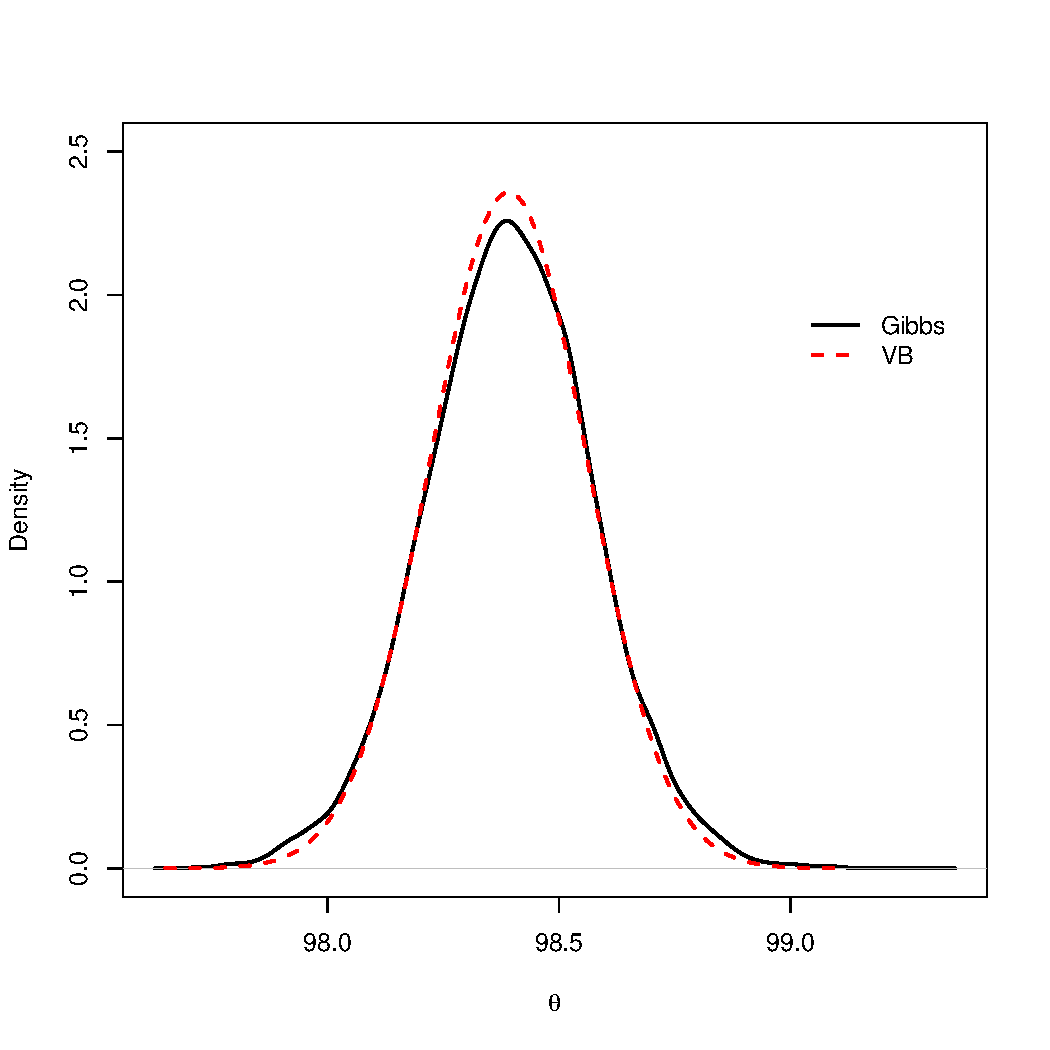
\includegraphics[height=5.2cm,angle=0]{plots/simpleVB_martheta.pdf}
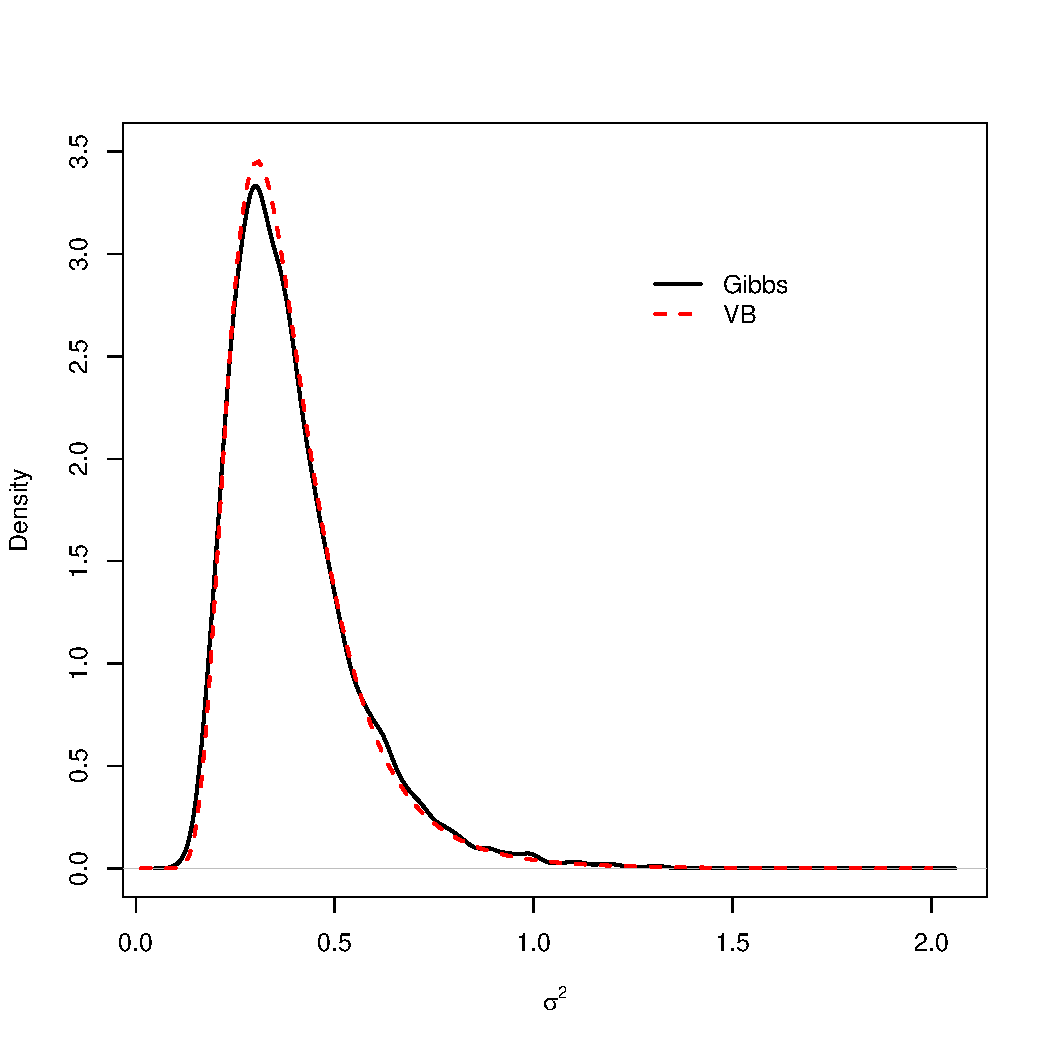
\includegraphics[height=5.2cm,angle=0]{plots/simpleVB_marsigma2.pdf}
\end{itemize}
}



\frame{
\sffamily
\frametitle{Variational algorithms}
\begin{itemize}
\item {\bf Example (Gaussian distributions with unknown mean and variance):}  Comparing the joint distributions.
\begin{center}
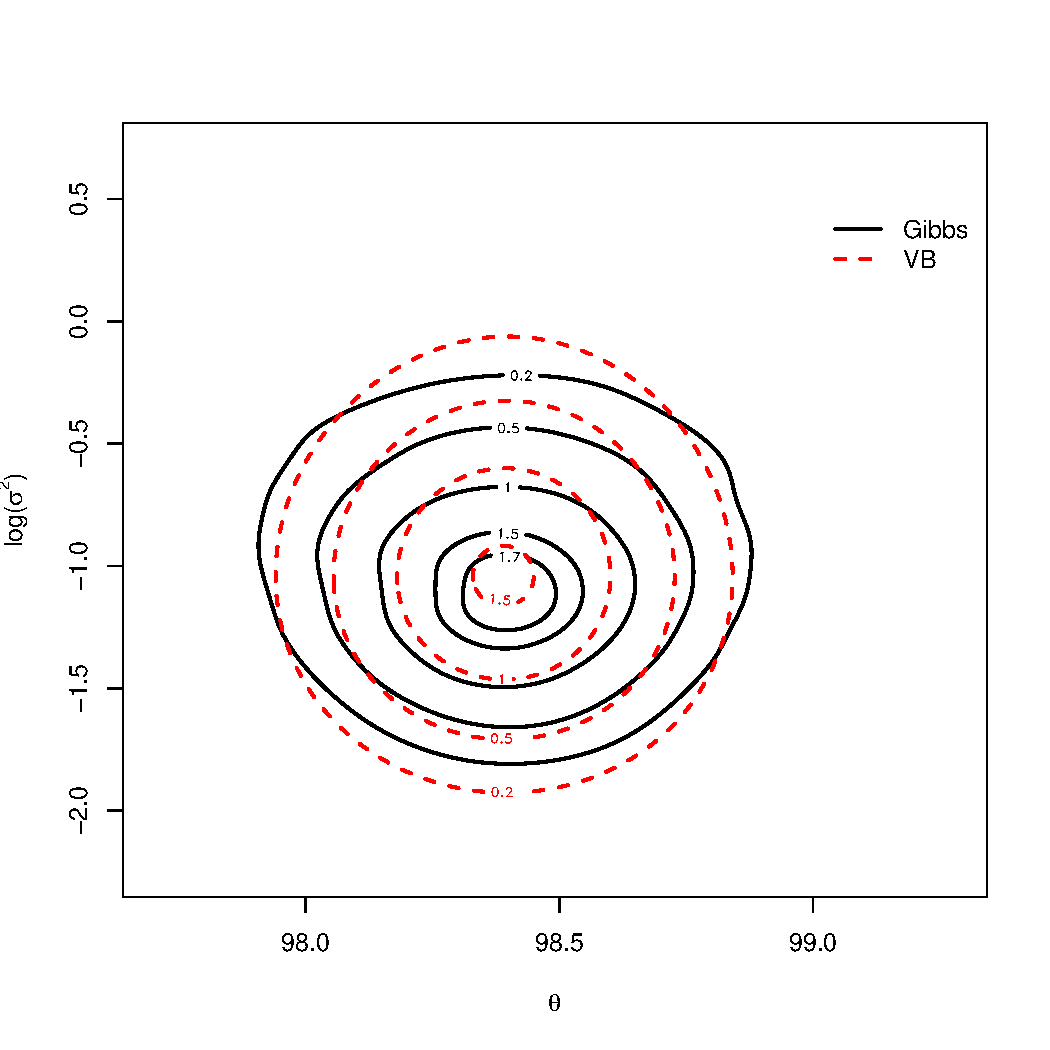
\includegraphics[height=6.5cm,angle=0]{plots/simpleVB_joint.pdf}
\end{center}
\end{itemize}
}




\frame{
\sffamily
\frametitle{Variational algorithms in exponential families}
\begin{itemize}
\item {\bf Example (Mixture models):  }  Recall the two-component Gaussian mixture model where
$$
y_i \mid \xi_i, \theta_1, \sigma_1^2, \theta_2, \sigma_2^2 \sim \normal(y_i \mid \theta_{\xi_i}, \sigma_{\xi_i}^2) 
$$
with $\Pr(\xi_i = 1 \mid \omega) = \omega = 1 - \Pr(\xi_i = 2 \mid \omega)$, $\omega \sim \bet(1, 1)$, $\theta_i \sim \normal(\mu,\tau^2)$ and $\sigma^2_i \sim \IGam(a, c)$.

\vspace{1mm}

For the purpose of deriving the variational algorithm, the best way to write the joint distribution of data and parameters is
\begin{multline*}
\left[ \prod_{i=1}^{n} \prod_{k=1}^{2} \left\{ p(y_i \mid \theta_k, \sigma_k^2 \right\}^{\ind_{(\xi_i=k)}} \right]  \\
%
\left[ \omega^{1 + \sum_{i=1}^{n}\ind_{(\xi_i=1)}} (1-\omega)^{1+ \sum_{i=1}^{n}\ind_{(\xi_i=2)}} \right]  \\
%
\left[ \prod_{k=1}^{2} \normal(\theta_k \mid \mu, \tau^2)  \IGam(\sigma^2_k \mid a, c) \right]
\end{multline*}
\end{itemize}
}







\frame{
\sffamily
\frametitle{Variational algorithms in exponential families}
\begin{itemize}
\item {\bf Example (Mixture models, cont):  }  The variational approximation in this case is given by
$$
q_{\gamma_1, \gamma_2}(\omega) \prod_{i=1}^{n} q_{\varpi_i}\left( \xi_i  \right) \prod_{k=1}^{2} q_{\eta_{k,1}, \eta_{k,2}}(\theta_k) \prod_{k=1}^{2} q_{\nu_{k,1}, \nu_{k,2}}\left( \sigma^2_k \right),
$$
where 
\begin{align*}
q_{\gamma_1, \gamma_2}(\omega) &= \bet(\omega \mid \gamma_1, \gamma_2) \\
q_{\varpi_i}\left( \xi_i = 1  \right) &= 1- q_{\varpi_i}\left( \xi_i = 2  \right) = \varpi_i  ,  \\
q_{\eta_{k,1}, \eta_{k,2}}(\theta_k)  &= \normal(\theta_k \mid \eta_{k,1}, \eta_{k,2})  ,  \\
q_{\nu_{k,1}, \nu_{k,2}}\left( \sigma^2_k \right) &= \IGam\left( \sigma^2_k \mid \nu_{k,1}, \nu_{k,2} \right)  .
\end{align*}
\end{itemize}
}






\frame{
\sffamily
\frametitle{Variational algorithms in exponential families}
\begin{itemize}
\item {\bf Example (Mixture models, cont):  }  The corresponding variational updates become
\begin{itemize}
\item For $\omega$,
{\scriptsize \begin{align*}
\gamma_1^{(b)}  &= 1 + \sum_{i=1}^{n} \varpi_i^{(b-1)}  ,    &  \gamma_2^{(b)}  &= 1 + n - \sum_{i=1}^{n} \varpi_i^{(b-1)}  .
\end{align*}}

\item For $\theta_1$,
{\scriptsize \begin{align*}
\eta_{1,1}^{(b)}  &= \frac{\frac{\nu_{1,1}^{(b-1)}}{\nu_{1,2}^{(b-1)}} \sum_{i=1}^{n} y_i \varpi_i^{(b-1)} + \frac{\mu}{\tau^2}}
{\frac{\nu_{1,1}^{(b-1)}}{\nu_{1,2}^{(b-1)}} \sum_{i=1}^{n} \varpi_i^{(b-1)} + \frac{1}{\tau^2}}   ,   
%
&  \eta_{1,2}^{(b)}  &= \frac{1}
{\frac{\nu_{1,1}^{(b-1)}}{\nu_{1,2}^{(b-1)}} \sum_{i=1}^{n} \varpi_i^{(b-1)} + \frac{1}{\tau^2}}  .
\end{align*}}
The formulas for $\theta_2$ are analogous but replace $\varpi_i$ with $1-\varpi_i$.
\end{itemize}
\end{itemize}
}


\frame{
\sffamily
\frametitle{Variational algorithms in exponential families}
\begin{itemize}
\item {\bf Example (Mixture models, cont):  }  
\begin{itemize}
\item For $\sigma_1^2$,
{\scriptsize \begin{align*}
\nu_{1,1} &= a + \frac{1}{2} \sum_{i=1}^{n} \varpi^{(b-1)}_i    \\
\nu_{1,2} &= c + \frac{1}{2} \sum_{i=1}^{n} \varpi^{(b-1)}_i \left\{  y_i^2 - 2 y_i \eta_{1,1}^{(b)} + \eta_{1,2}^{(b)} + \eta_{1,1}^{2(b)} \right\}
\end{align*}}
The formulas for $\sigma^2_2$ are analogous but replace $\varpi_i$ with $1-\varpi_i$.

\vspace{1.5mm}

\item For $\xi_i$,
{\scriptsize \begin{multline*}
\varpi^{(b)}_i \propto \exp \left\{ \Psi \left( \gamma_1^{(b)} \right) - \Psi \left( \gamma_1^{(b)}  +\gamma_2^{(b)} \right) 
%
+ \frac{1}{2} \left[ \Psi \left( \nu_{k,1}^{(b)} \right) - \log \nu_{k,2}^{(b)} \right]  \right.  \\
%
\left. 
-\frac{\nu_{k,1}^{(b)}}{2 \nu_{k,2}^{(b)}} \left[ y_i^2 - 2y_i \eta_{k,1}^{(b)} +  \eta_{k,2}^{(b)} + \eta_{k,1}^{2(b)}
%
\right]
\right\}
\end{multline*}}
where $\Psi$ denotes the digamma function.
\end{itemize}
\end{itemize}
}



\frame{
\sffamily
\frametitle{Variational algorithms in exponential families}
\begin{itemize}
\item {\bf Example (Mixture models, cont):  }  The algorithm can be naturally extended to mixtures with a larger number of components, and even to nonparametric mixtures.  

\vspace{1mm}

The following two slides show results for a slightly more convoluted location scale mixture under a finite Dirichlet process mixture model \cite{BlJo06} for the \texttt{galaxy} dataset \cite{roeder1990density} (available in the \texttt{DPpackage} library for \texttt{R}).  They illustrate some of the disadvantages of variational approximation when compared to ``equivalent'' Gibbs sampling algorithms.
\end{itemize}
}




\frame{
\sffamily
\frametitle{Gibbs vs.\ variational algorithms for location mixtures of normals}
Density estimates
\begin{center}
\begin{tabular}{cc}
Blocked Gibbs sampler  &  Variational approximation \\
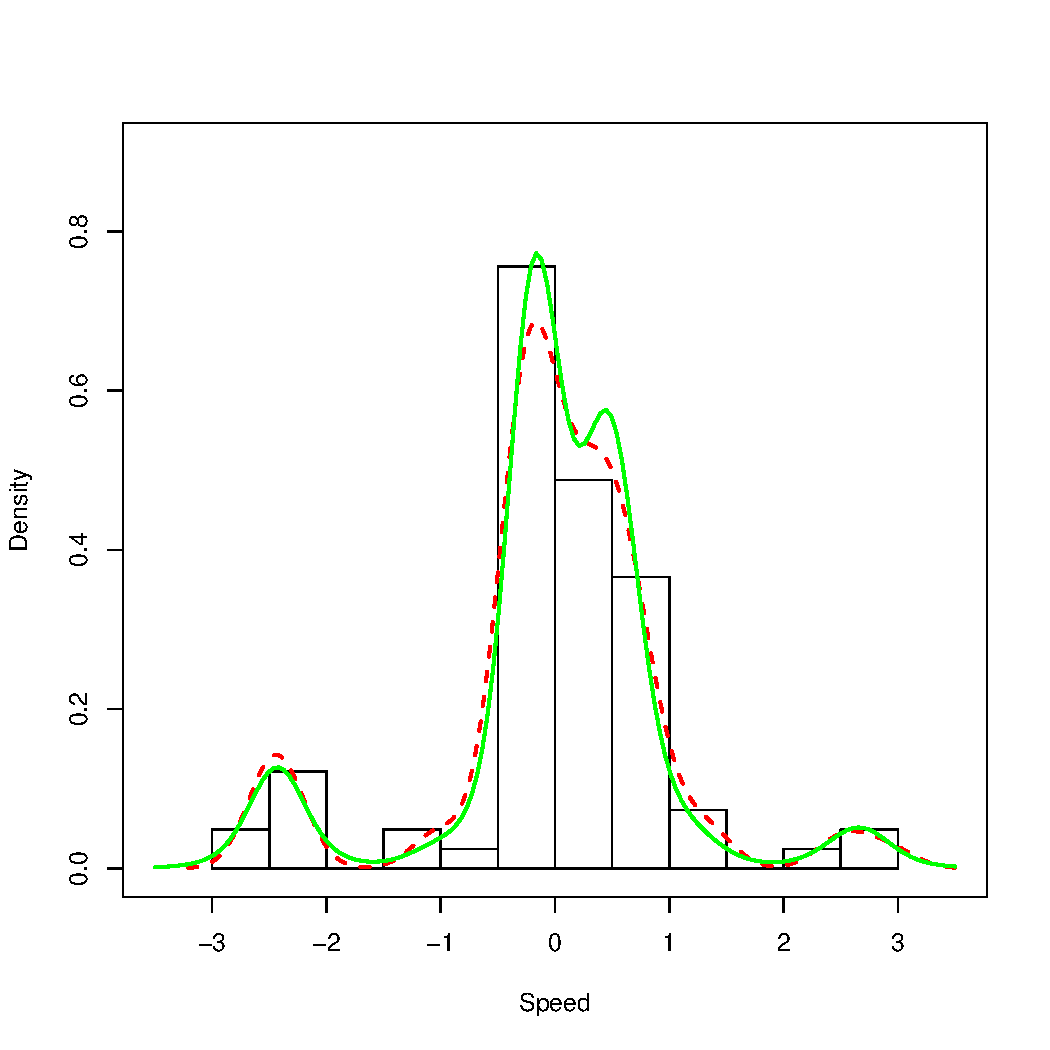
\includegraphics[height=5.2cm,angle=0]{plots/densityest_galaxy_lmfs_blockedgibbs.pdf}  &
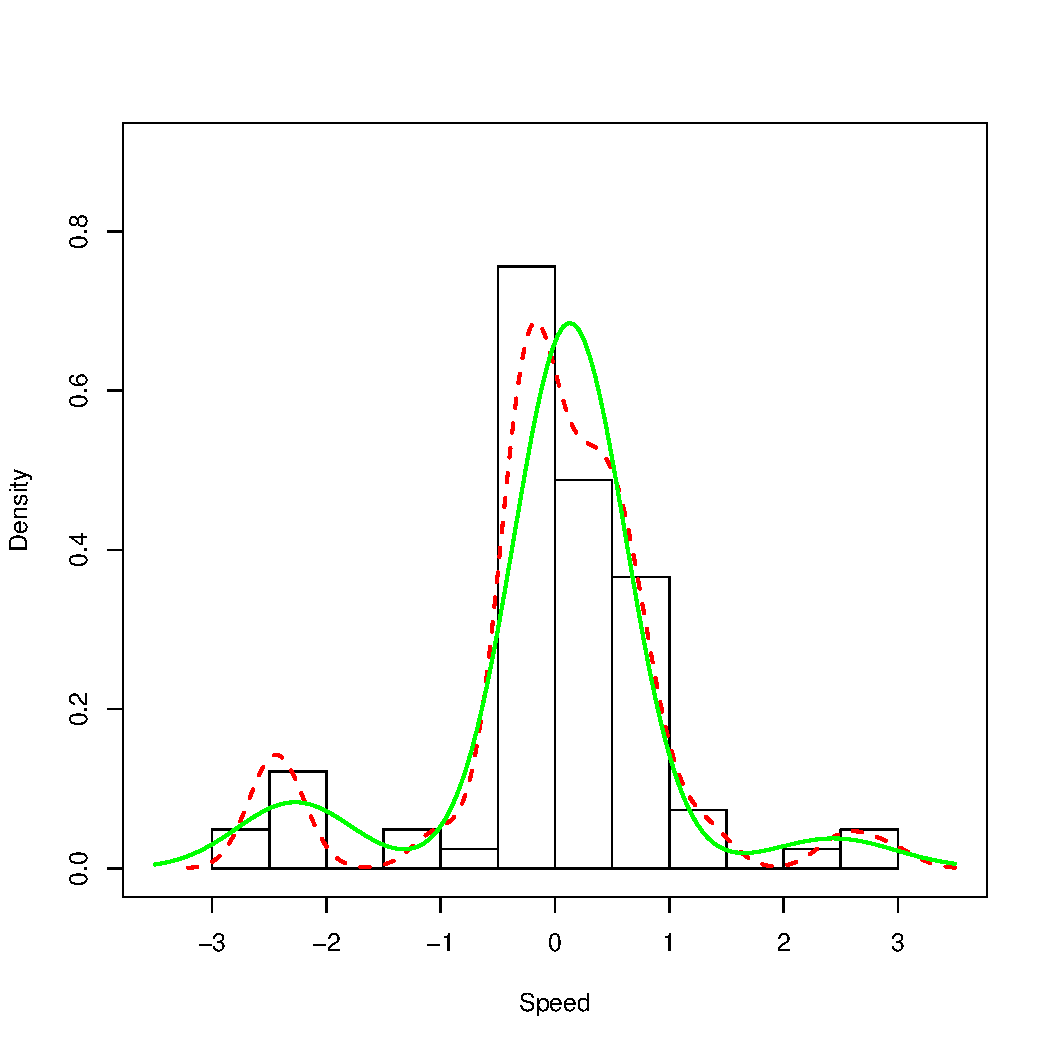
\includegraphics[height=5.2cm,angle=0]{plots/densityest_galaxy_lmfs_variational.pdf}
\end{tabular}
\end{center}
}


\frame{
\sffamily
\frametitle{Gibbs vs.\ variational algorithms for location mixtures of normals}
\begin{center}
Pairwise clustering probabilities
\begin{tabular}{cc}
Blocked Gibbs sampler  &  Variational approximation \\
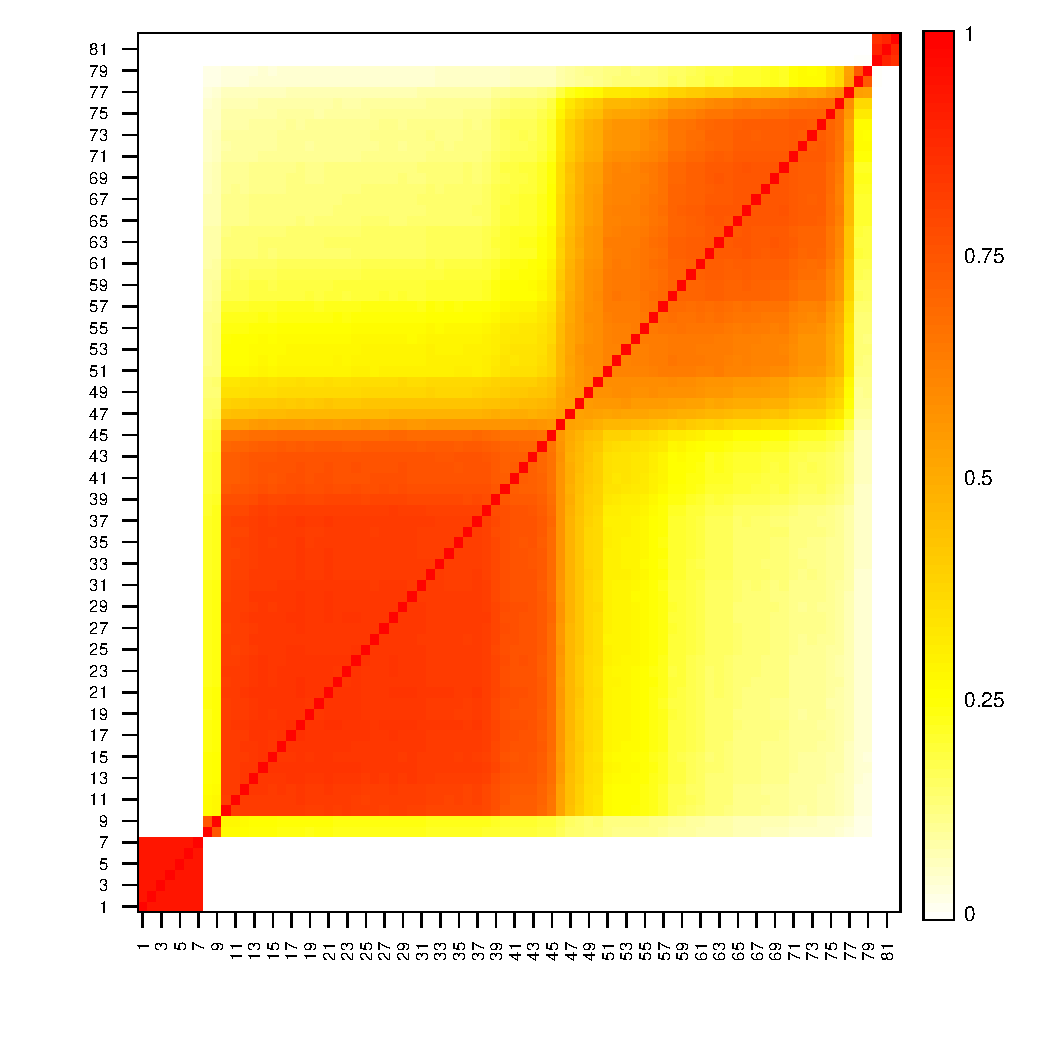
\includegraphics[height=5.2cm,angle=0]{plots/pairwise_galaxy_lmfs_blockedgibbs.pdf}  &
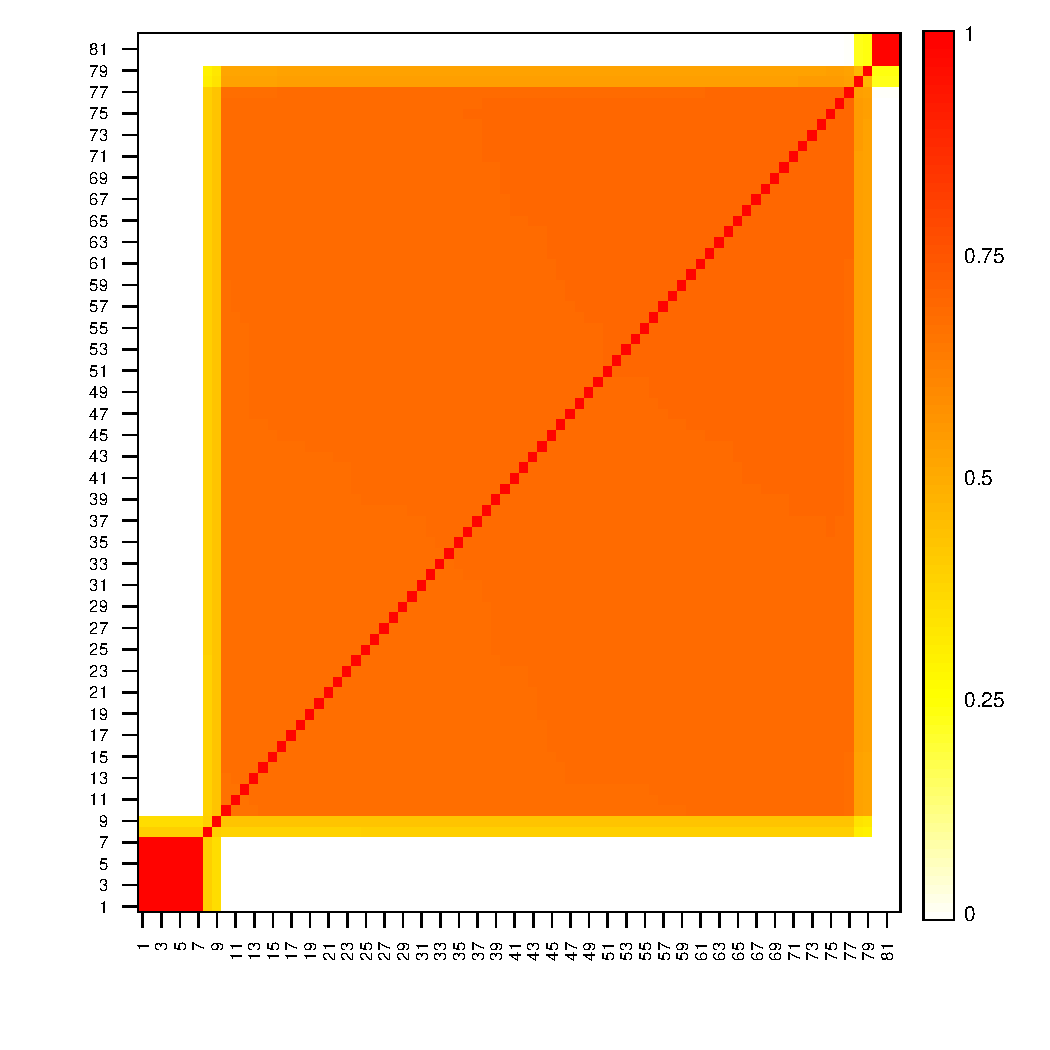
\includegraphics[height=5.2cm,angle=0]{plots/pairwise_galaxy_lmfs_variational.pdf}
\end{tabular}
\end{center}
}






\frame{
\sffamily
\frametitle{Some concluding remarks about variational algorithms}
\begin{itemize}

\item The minimization of $K(q || p)$ can also be justified as maximizing the bound on the log marginal likelihood:
\begin{align*}
\log p(\bfy) \ge \E_{q} \left\{ \log p(\bftheta, \bfy) \right\} - \E_q \left\{ \log q_{\bfeta}(\bftheta) \right\}
\end{align*}
The gap in the bound is precisely the divergence between $q_{\bfeta}$ and the true posterior.  This value of this gap is usually monitored to assess convergence of the algorithm.

\item Variational Bayes works well at approximating the marginal posteriors of the parameters on which it is derived, but typically fails for joint distributions/transformations involving multiple parameters.

\item For complex models variational algorithms tend to get stuck in local modes.  It is very important to perform multiple runs from \textit{overdispersed} initial values and verify that the algorithm converges to the same set of values.
\end{itemize}
}







\frame{
\sffamily
\frametitle{The Laplace approximation}
\begin{itemize}
\item An alternative to variational approximations are Laplace approximations.

\item The Laplace approximation is a simple yet powerful asymptotic expansion of the posterior distribution that goes back to Laplace in 1774!

\item There are different variants of the technique, but the main argument is similar in all cases:  Start by assuming that $y_1, \ldots, y_n$ are independent and identically distributed with $y_i \mid \bftheta \sim p(y_i \mid \bftheta)$ so that the posterior takes the form
$$
%  p(\bfy \mid \bftheta) p(\bftheta)
p( \bftheta \mid \bfy ) \propto \exp \left\{ - n h_n(\bftheta) \right\} ,
$$
where $h_n(\bftheta) = -\frac{1}{n} \sum_{i=1}^{n} \log p(y_i \mid \bftheta) - \frac{p(\bftheta)}{n}$.
\end{itemize}
}




\frame{
\sffamily
\frametitle{The Laplace approximation}
\begin{itemize}
\item Now, do a second order expansion of $h_n(\bftheta)$ around a point $\bftheta_0$ and write
\begin{multline*}
h_n(\bftheta) = h_n(\bftheta_0) + \left[ \nabla h_n \left( \bftheta_0 \right) \right]^{T} \left[ \bftheta - \bftheta_0 \right] \\
%
+ \frac{1}{2} \left[ \bftheta - \bftheta_0 \right]^{T} \left[ \nabla \nabla h_n \left( \bftheta_0 \right) \right] \left[ \bftheta - \bftheta_0 \right]  + R_n(\bftheta, \bftheta_0)  ,
\end{multline*}
where $\nabla h_n \left( \bftheta \right)$ is the gradient of $h_n$ and $\nabla \nabla h_n \left( \bftheta \right)$ is the Hessian matrix of $h$.

\item It is not difficult to show that, under standard regularity conditions, $ \lim_{n \to \infty} R_n(\bftheta, \bftheta_0) = 0$.
\end{itemize}
}




\frame{
\sffamily
\frametitle{The Laplace approximation}
\begin{itemize}
\item The previous argument suggests the approximation
\begin{multline*}
p( \bftheta \mid \bfy ) \overset{\boldsymbol{\cdot}}{\propto} \exp \left\{ - n
 \left[ \nabla h_n \left( \bftheta_0 \right) \right]^{T} \left[ \bftheta - \bftheta_0 \right] \right. \\
%
\left. - \frac{n}{2} \left[ \bftheta - \bftheta_0 \right]^{T} \left[ \nabla \nabla h_n \left( \bftheta_0 \right) \right] \left[ \bftheta - \bftheta_0 \right]   \right\}
\end{multline*}
which corresponds to a Gaussian kernel!

\item Note that the contribution of the prior drops out faster than the contribution from the likelihood.  Therefore, alternatively,
\begin{multline*}
p( \bftheta \mid \bfy )  \overset{\boldsymbol{\cdot}}{\propto} \exp \left\{ 
 \left[ \left. \nabla \log p\left( \bfy \mid \bftheta \right) \right|_{\bftheta= \bftheta_0}\right]^{T} \left[ \bftheta - \bftheta_0 \right] \right. \\
%
\left. - \frac{1}{2} \left[ \bftheta - \bftheta_0 \right]^{T} \left[ \left. - \nabla \nabla \log p \left( \bfy \mid \bftheta \right)  \right|_{\bftheta = \bftheta_0} \right] \left[ \bftheta - \bftheta_0 \right]   \right\} .
\end{multline*}
\end{itemize}
}

%where $- \nabla \nabla p \left( \bfy \mid \bftheta \right)  \right|_{\bftheta = \bftheta_0}$ is the 


\frame{
\sffamily
\frametitle{The Laplace approximation}
\begin{itemize}
\item Typically $\bftheta_0$ is taken to be either the MLE of $\bftheta$ or the maximum a posteriori, leading to simplifications.
\begin{itemize}
\item For example, discarding the contribution of the likelihood and letting $\bftheta_0 = \hat{\bftheta}$ we have 
\begin{multline*}
p( \bftheta \mid \bfy )  \overset{\boldsymbol{\cdot}}{\propto} \\
%
\exp \left\{ - \frac{1}{2} \left[ \bftheta - \hat{\bftheta} \right]^{T} \left[ \left. - \nabla \nabla \log p \left( \bfy \mid \bftheta \right)  \right|_{\bftheta = \hat{\bftheta}} \right] \left[ \bftheta - \hat{\bftheta} \right]   \right\}
\end{multline*}
where the matrix $\left. - \nabla \nabla \log p \left( \bfy \mid \bftheta \right)  \right|_{\bftheta = \hat{\bftheta}}$ is called the \textit{observed} information matrix.  That is 
$$
\bftheta \mid \bfy \overset{\boldsymbol{\cdot}}{\sim} \normal\left( \hat{\bftheta} , \left[ \left. - \nabla \nabla \log p \left( \bfy \mid \bftheta \right)  \right|_{\bftheta = \hat{\bftheta}} \right]^{-1} \right)
$$
\end{itemize}

\item This last version of the approximation is the basis for ``Bayesian CLT'', as well as for the derivation of the BIC.
\end{itemize}
}




\frame{
\sffamily
\frametitle{The Laplace approximation}
\begin{itemize}
\item Although technically the result is valid for any parameterization, maing appropriate transformations (e.g., logarithm, logit) might improve the accuracy.

\item The Laplace approximation can be very accurate for large $n$, but in complicated hierarchical models with a large number of hyperparameters the approximation can be very poor!

\item When the posterior moments are available in closed form, it might simply be better to use the posterior mean and variance as the moments for the normal approximation.

\item Even if they are not very accurate, Laplace approximations are sometimes used to guide the construction of proposal distributions in some of the Monte Carlo schemes discussed before.
\end{itemize}
}




\frame{
\sffamily
\frametitle{The Laplace approximation}
\begin{itemize}
\item {\bf Example (Poisson-Gamma models): }  Consider data $y_1, \ldots, y_n$ where $y_i \sim \Poi (\lambda)$ and $\lambda \sim \Gam(a, b)$  The posterior distribution (which is known to be a $\Gam\left( a + \sum_{i=1}^{n} y_i , n + b \right)$ distribution) can be written as $p(\lambda \mid \bfy) \propto \left\{ - n h_n(\lambda) \right\}$ where 
$$
h_n(\lambda) = - \lambda \frac{n+b}{n} + \frac{a - 1 + \sum_{i=1}^{n} y_i}{n} \log \lambda .
$$

It is easy to se that the posterior mode in this case is $\tilde{\lambda} = \frac{a - 1 + \sum_{i=1}^{n} y_i}{n+b}$.  Also $- \frac{\partial^2 h_n}{\partial \lambda^2} = \frac{a - 1 + \sum_{i=1}^{n} y_i}{n} \frac{1}{\lambda^2}$, which leads 
$$
\lambda \mid \bfy \overset{\boldsymbol{\cdot}}{\sim} \normal \left(  \frac{a - 1 + \sum_{i=1}^{n} y_i}{n+b} , \frac{\left\{ a - 1 + \sum_{i=1}^{n} y_i \right\}}{(n+b)^2} 
\right)
$$
\end{itemize}
}





\frame{
\sffamily
\frametitle{The Laplace approximation}
\begin{itemize}
\item {\bf Example (Poisson-Gamma models, cont): }  Alternatively, if we discard the prior and center the approximation on the MLE we get the familiar expression
$$
\lambda \mid \bfy \overset{\boldsymbol{\cdot}}{\sim} \normal \left(  \frac{1}{n} \sum_{i=1}^{n} y_i ,   \sum_{i=1}^{n} \frac{y_i}{n^2}   
\right).
$$
(Note that this is equivalent to setting $a=1$ and $b=0$ in the first approximation).

\vspace{1mm}

If we are interested in approximating the posterior mean then we have
\begin{center}
\begin{tabular}{|c|c|} \hline
Exact            &   $\frac{a + \sum_{i=1}^{n}y_i}{b + n}$      \\
Like + Prior   &  $\frac{a -1 + \sum_{i=1}^{n}y_i}{b + n}$   \\
Like only       &  $\frac{\sum_{i=1}^{n}y_i}{n}$                   \\ \hline
\end{tabular}
\end{center}

\vspace{1mm}

If $a$ is large and $n$ small, the differences can be substantial!
\end{itemize}
}





\frame{
\sffamily
\frametitle{The Laplace approximation}
\begin{itemize}
\item {\bf Example (Poisson-Gamma models): }  The following graphs show a comparison of the two approximations against the true posterior for $a=2$, $b=1/5$ and $\bar{y} = 2$.

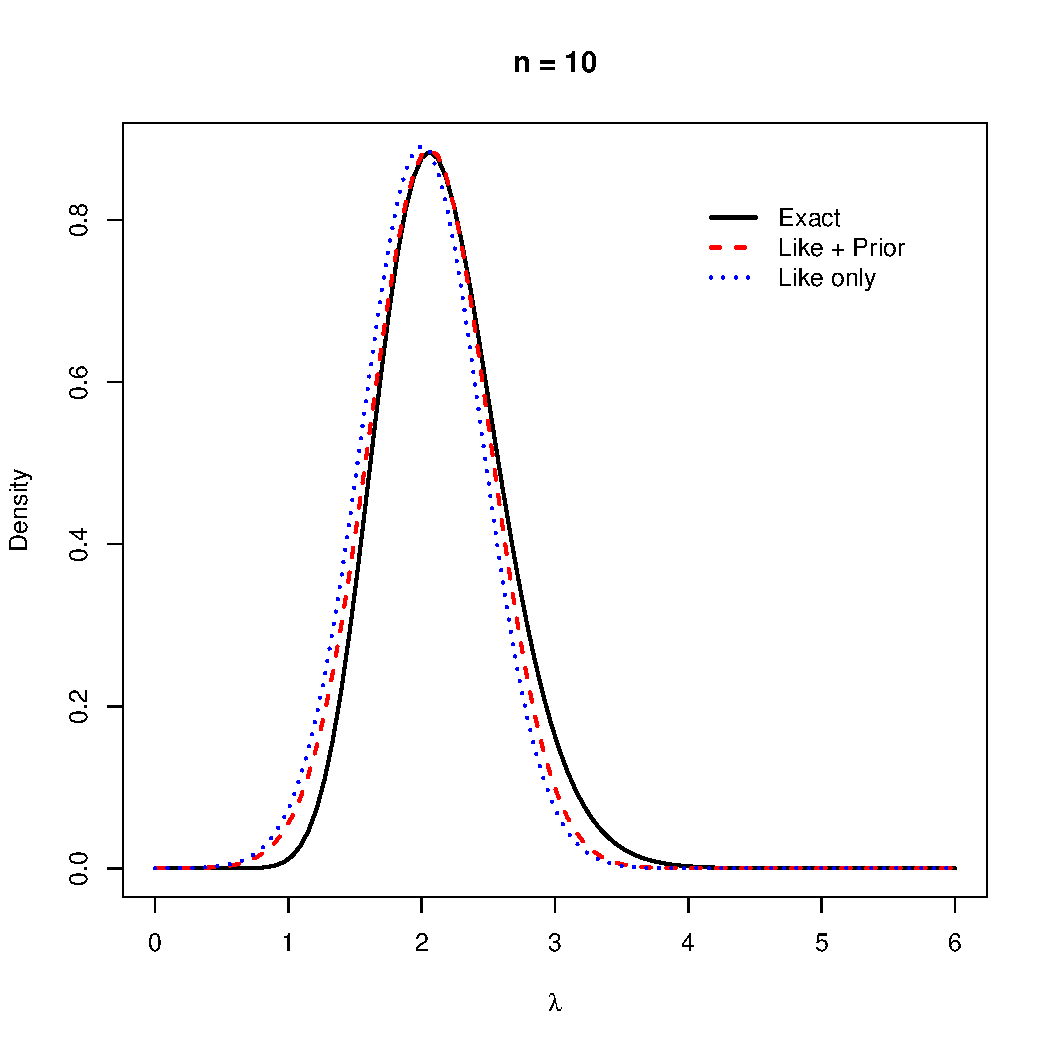
\includegraphics[height=5.2cm,angle=0]{plots/laplaceapprox_poissongamma_n10.pdf}
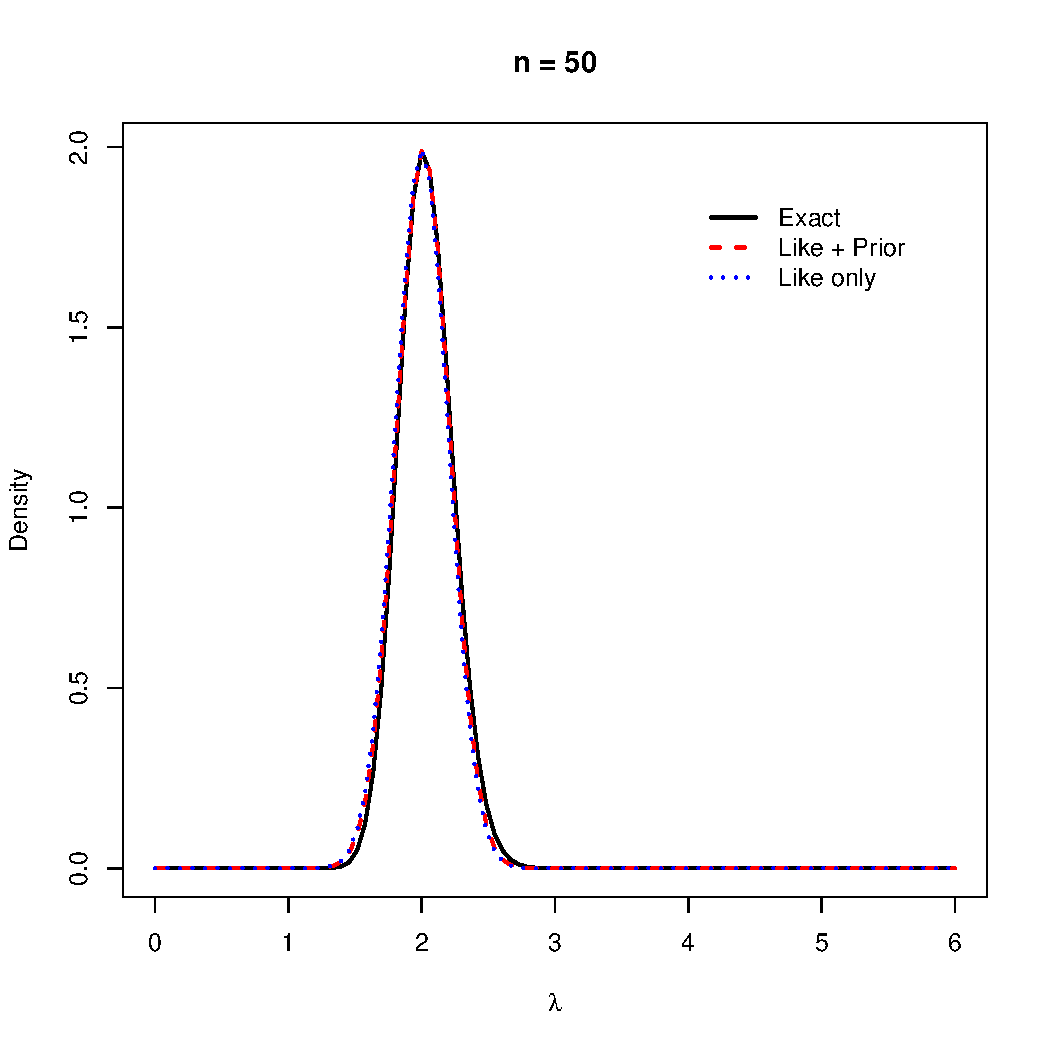
\includegraphics[height=5.2cm,angle=0]{plots/laplaceapprox_poissongamma_n50.pdf}

\end{itemize}
}





\frame{
\sffamily
\frametitle{The Laplace approximation}
\begin{itemize}
\item {\bf Example (Poisson-Gamma models): }  The following table compares the exact posterior probability of the interval $(l,u)$ against these two approximation for different intervals and sample sizes.

\begin{center}
\begin{tabular}{ccccc}
  $(l,u)$   &   $n$   &   Exact   &   Like + Prior   &  Like only \\ \hline\hline
  $(1.5, 2.8)$     &              &   0.849   &   0.844   &   0.831   \\
  $(1.8, 2.3)$   &  $10$ &   0.420   &   0.422   &   0.421   \\
  $(2.5, \infty)$ &              &   0.218   &   0.163   &    0.132  \\ \hline
  $(1.5, 2.8)$     &              &   0.998   &   0.995   &   0.994   \\
  $(1.8, 2.3)$   &  $50$ &   0.783   &   0.780   &   0.775   \\
  $(2.5, \infty)$ &              &   0.014   &  0.007    &   0.006   \\ \hline
\end{tabular}
\end{center}
\end{itemize}
}



\frame{
\sffamily
\frametitle{Integrated Nested Laplace Approximations}
\begin{itemize}
\item INLA is designed for hierarchical models:
\begin{align*}
y_i \mid \theta_i, \bfeta_1 &\sim p(y_i \mid \theta_i, \bfeta_1)    &    \bftheta \mid \bfeta_2 & \sim \normal \left( \mathbf{0} , \mathbf{Q}(\bfeta_2)  \right)  ,
\end{align*}
where $\bfeta = (\bfeta_1, \bfeta_2) \sim p(\bfeta_1, \bfeta_2)$ and $m = \mbox{dim} (\bfeta_1) + \mbox{dim} (\bfeta_2)$ is small (usually $\le 6$).

\item Particularly useful if $\mathbf{Q}(\bfeta_2)$ is sparse.

\item Goal is to provide approximations to 
$$
p(\theta_i \mid \bfeta, \bfy) = \int p(\theta_i \mid \bfeta, \bfy) p(\bfeta \mid \bfy) \dd \bfeta
$$
and
$$
p(\eta_j \mid \bfy) = \int p(\eta \mid \bfy) \dd \bfeta_{-j} .
$$

\item Uses Laplace approximations twice (hence the name).
\end{itemize}
}






\frame{
\sffamily
\frametitle{Approximating $p(\bfeta \mid \bfy)$}
\begin{itemize}
\item Start by approximating $p(\bfeta \mid \bfy)$ by
$$
\tilde{p}(\bfeta \mid \bfy) \propto \left. \frac{p(\bftheta, \bfeta, \bfy)}{\tilde{p}_G(\bftheta \mid \bfeta, \bfy)} \right|_{\bftheta = \hat{\bftheta}(\bfeta)}
$$
where $\tilde{p}_G(\bftheta \mid \bfeta, \bfy)$ is a Gaussian approximation to the full conditional of $\bftheta$
$$
p(\bftheta \mid \bfeta, \bfy) \propto \exp \left\{ -\frac{1}{2} \bftheta^T \mathbf{Q}\left(\bfeta_2\right) \bftheta + \sum_{i} \log\left\{ p(y_i \mid \theta_i, \bfeta_1) \right\} \right\}
$$
and $\hat{\bftheta}(\bfeta) = \arg\max_{\bftheta} p(\bftheta \mid \bfeta, \bfy)$.  This is just the Laplace approximation around the posterior mode.
\end{itemize}
}







\frame{
\sffamily
\frametitle{Approximating $p(\bfeta \mid \bfy)$}
\begin{itemize}
\item Generally speaking $\tilde{p}(\bfeta \mid \bfy)$ will not be tractable even if $\tilde{p}_G(\bftheta \mid \bfeta, \bfy)$ is.  Hence, this approximation by itself is not too helpful for computing an approximation to $p(\theta_i \mid \bfeta, \bfy)$.

\item We go one step forward and approximate the approximation using a discrete set of points,
$$
\tilde{p}^{*}(\bfeta \mid \bfy) = \sum_{i_1 \in \mathcal{I}_1} \cdots \sum_{i_m \in \mathcal{I}_m} w_{i_1, \cdots, i_m} \delta_{(\tilde{\eta}_{i_1}, \ldots, \tilde{\eta}_{i_m})} (\bfeta)
$$
where the points $(\tilde{\eta}_{i_1}, \ldots, \tilde{\eta}_{i_m})$ for $(i_1, \ldots, i_m) \in \mathcal{I}_1 \times \cdots \times \mathcal{I}_m$ form a regular grid and
$$
w_{i_1, \cdots, i_m} \propto \tilde{p}^{*}(\tilde{\eta}_{i_1}, \ldots, \tilde{\eta}_{i_m} \mid \bfy)
$$
\item To select the grid points we use a second Laplace expansion (in this case of $\tilde{p}(\bfeta \mid \bfy)$).  See next slide.
\end{itemize}
}






\frame{
\sffamily
\frametitle{Approximating $p(\bfeta \mid \bfy)$}
\begin{center}
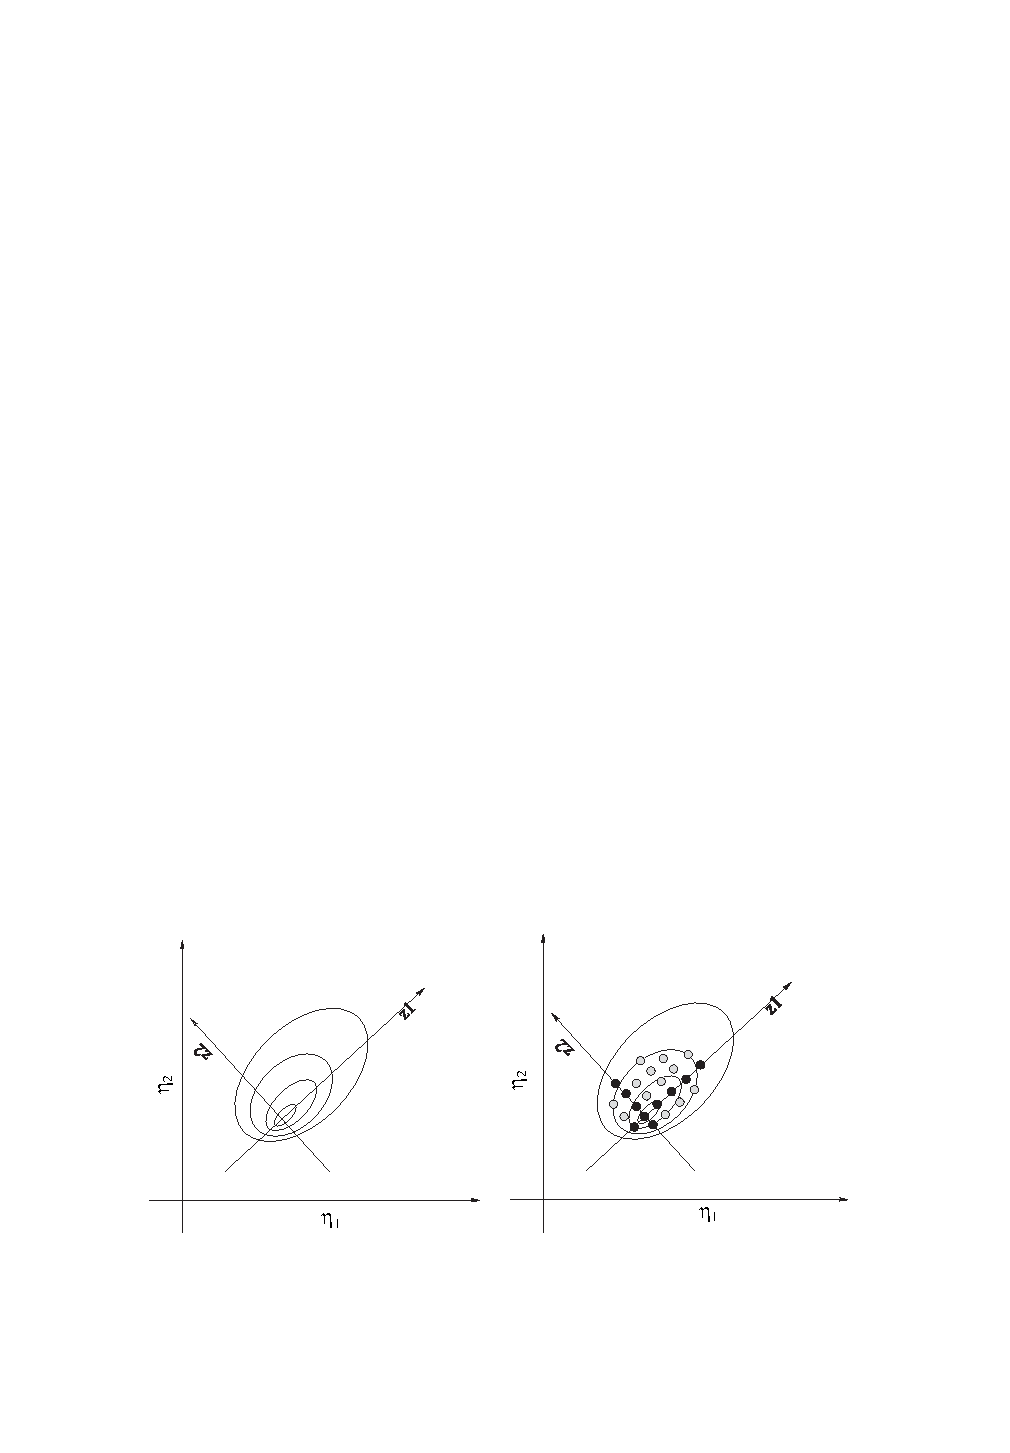
\includegraphics[width=11cm,angle=0]{plots/INLA.pdf}  \\
\hfill From \cite{rue2009approximate}.
\end{center}
}







\frame{
\sffamily
\frametitle{Approximating $p(\eta_i \mid \bfy)$}
\begin{itemize}
\item It is natural to approximate $p(\eta_j \mid \bfy)$ by 
$$
\tilde{p}(\eta_j \mid \bfy) = \int \tilde{p}(\eta \mid \bfy) \dd \bfeta_{-j}  .
$$

\item The integral can be computed using standard numerical integration techniques.

\item However, it is much more efficient to construct the numerical integrator by reusing the grid of values used in the definition $\tilde{p}^{*}(\bfeta \mid \bfy)$ (which is aligned with the principal axes of the distribution) rather than a completely new grid aligned to the original axes.
\end{itemize}
}












\frame{
\sffamily
\frametitle{Approximating $p(\theta_i \mid \bfeta, \bfy)$}
\begin{itemize}
\item If we had access to $p(\theta_i \mid \bfeta, \bfy)$ in closed form, the approximation $\tilde{p}^{*}(\bfeta \mid \bfy)$ could be used to compute $\hat{p}(\theta_i \mid \bfy)$ as
\begin{align*}
\hat{p}(\theta_i \mid \bfy) &= \int p(\theta_i \mid \bfeta, \bfy) \tilde{p}^{*}(\bfeta \mid \bfy)  \dd \bfeta \\
& = \sum_{i_1 \in \mathcal{I}_1} \cdots \sum_{i_m \in \mathcal{I}_m} w_{i_1, \cdots, i_m} 
p(\theta_i \mid (\tilde{\eta}_{i_1}, \ldots, \tilde{\eta}_{i_m}), \bfy)
\end{align*}

\item However, in $p(\theta_i \mid \bfeta, \bfy)$ is not available in closed form so we need to first approximate by $\hat{p}(\theta_i \mid \bfeta, \bfy)$.  One option is to reuse the Laplace approximation $\tilde{p}_G(\bftheta \mid \bfeta, \bfy)$ we already computed for getting $\hat{p}(\theta_i \mid \bfy)$.  Then
$$
\hat{p}^{*}(\theta_i \mid \bfy) = \sum_{i_1 \in \mathcal{I}_1} \cdots \sum_{i_m \in \mathcal{I}_m} w_{i_1, \cdots, i_m} 
\tilde{p}_G(\theta_i \mid (\tilde{\eta}_{i_1}, \ldots, \tilde{\eta}_{i_m}), \bfy)
$$
\end{itemize}
}




\frame{
\sffamily
\frametitle{Approximating $p(\theta_i \mid \bfeta, \bfy)$}
\begin{itemize}
\item Reusing $\tilde{p}_G(\bftheta \mid \bfeta, \bfy)$ is expedient, but does not account for skewness and other features of the data.

\item An alternative is to use another Laplace expansion
$$
\tilde{p}_{LA}(\theta_i \mid \bfeta, \bfy) \propto \left. \frac{p(\bftheta, \bfeta, \bfy)}{\tilde{p}_{GG}(\bftheta_{-i} \mid \theta_i, \bfeta, \bfy)} \right|_{\bftheta_{-i} = \hat{\bftheta}_{-i} (\theta_i, \bfeta)}
$$
where $\tilde{p}_{GG}(\bftheta_{-i} \mid \theta_i, \bftheta, \bfy)$ is a Gaussian approximation to $(\bftheta_{-i} \mid \theta_i, \bfeta, \bfy)$ (which is different from the full conditional obtained from $\bftheta \mid \bfeta, \bfy$).
\end{itemize}
}

\frame{
\sffamily
\frametitle{Laplace-based methods and NIMBLE}

\begin{itemize}
\item Currently your software options are R-INLA and the related TMB software.
\item NIMBLE is very close to having automatic differentiation, which is important for Laplace-based methods as they need gradients.
\item At that point, one of our target algorithms will be INLA so we hope to see that in NIMBLE within a year.
\item Our hope is that by providing in NIMBLE, users can:
\begin{itemize}
\item use BUGS code to specify their model,
\item use distributions and model structures not provided in R-INLA, and
\item more readily compare results with other algorithms.
\end{itemize}
\end{itemize}

}



\frame{
\sffamily
\frametitle{Learning objectives}
\begin{itemize}
\item Understand the landscape of current computational methods for
Bayesian inference; 
\item Understand the statistical and probabilistic principles behind the methods;
\item Understand the various MCMC alternatives and how to assess MCMC performance;
\item Be able to choose a method and software tool for a real-world problem; and
\item Be able to implement Bayesian inference using NIMBLE and Stan.
\end{itemize}
}

%\section{References}

{\tiny
\bibliographystyle{bka}
\bibliography{bayesiancomputation}
}




\section{Appendix}

\frame{
\sffamily
\frametitle{Stan example: Cox regression}
\begin{itemize}
\item {\bf Example (Cox regression):} Recall that standard Cox regression specifies the hazard function as:
$$ \lambda(t|z) = \lambda_0(t)\exp(z^\top \beta) $$
for an unspecified baseline hazard, $\lambda_0(t)$.

With right-censoring, one has the likelihood (for one patient):
$$
(\lambda_0(w_i) \exp(z_i^\top \beta))^{v_i} \exp\left(
   -\exp(z_i^\top \beta) \int_0^{w_i} \lambda_0(u)du \right)
   $$
   
   where $w_i$ is the minimum of the failure time and the censoring time for the patient and $v_i$ is 1 if the person is not censored.

It turns out this likelihood can be written as a Poisson distribution when one assumes piecewise constant baseline hazard -- we'll use this in the implementation.
\end{itemize}
}

\frame{
\sffamily
\frametitle{Stan example: Bayesian Cox regression}
\begin{itemize}
\item {\bf Example (Cox regression):} A Bayesian treatment requires either a prior for $\lambda_0(t)$ or use of the Kalbfleisch (1978) result that Cox's partial likelihood can be used as an approximation to an actual likelihood, with a prior placed simply on the regression coefficients.

Considering the fully Bayesian approach, a canonical solution has been to assume a piecewise constant hazard model with independent jumps at the failure times. The size of the jumps is centered on those in a parametric hazard model, $\lambda_0^*(t)$ (such as a Weibull) using a gamma distribution for conjugacy.
$$
\lambda_0(t)dt \sim \mbox{Gamma}(c\lambda_0^*(t)dt, c)
$$
This construction is called a gamma process.
\end{itemize}
}


\frame{
\sffamily
\frametitle{Stan example: Stan overview}
Stan focuses on HMC, so its primary computation is of the full log posterior density.
\begin{itemize}
\item \texttt{model} block of code uses imperative syntax (order matters) to encode calculation of log posterior.
\item BUGS-style distributional statements are allowed.
\item Stan also has its own language for encoding computation, including full linear algebra.
\end{itemize}

Stan generates C++ from the model code to implement HMC for the model and then compiles it to an executable, similar to NIMBLE. 

Note: Stan cannot handle discrete parameters (discrete data are fine), so any implementation would require marginalization over such parameters.

}

\frame{
\sffamily
\frametitle{Stan example: Stan overview}
Other blocks of Stan code for a model describe:
\begin{itemize}
\item \texttt{data}: input data and what NIMBLE calls constants
\item \texttt{transformed data}: fixed hyperparameters and transformations of input data
\item \texttt{parameters}: list of unknown parameters
\item \texttt{generated quantities}: posterior functionals of parameters and/or data

\end{itemize}

}

\begin{frame}[fragile] 
\sffamily
\frametitle{Stan example: Stan code for Cox regression}

Here's the core \texttt{model} block for Cox regression for the BUGS leukemia example.
{\footnotesize
\begin{verbatim}
model {
  beta ~ normal(0, 1000);
  for(j in 1:NT) {  ## unique times
    ## gamma process prior for baseline hazard, centered on exponential
    dL0[j] ~ gamma(c * r * (t[j + 1] - t[j]), c);
    for(i in 1:N) { ## patients
      if (Y[i, j] != 0)
         ## Poisson representation of likelihood with piecewise
         ## baseline hazard; Y[i,j] is observation process:
         ## Y[i,j]=1 if patient i is observed and 0 if censored
         dN[i, j] ~ poisson(Y[i, j] * exp(beta * Z[i]) * dL0[j]);
    }     
  }
}
\end{verbatim}
}

See \texttt{hmc-cox.R} for full Stan implementation.
\end{frame}


\end{document}


